% Options for packages loaded elsewhere
\PassOptionsToPackage{unicode}{hyperref}
\PassOptionsToPackage{hyphens}{url}
%
\documentclass[
]{book}
\title{Introduction to R for Biologists}
\author{Hena Ramay}
\date{2022-04-19}

\usepackage{amsmath,amssymb}
\usepackage{lmodern}
\usepackage{iftex}
\ifPDFTeX
  \usepackage[T1]{fontenc}
  \usepackage[utf8]{inputenc}
  \usepackage{textcomp} % provide euro and other symbols
\else % if luatex or xetex
  \usepackage{unicode-math}
  \defaultfontfeatures{Scale=MatchLowercase}
  \defaultfontfeatures[\rmfamily]{Ligatures=TeX,Scale=1}
\fi
% Use upquote if available, for straight quotes in verbatim environments
\IfFileExists{upquote.sty}{\usepackage{upquote}}{}
\IfFileExists{microtype.sty}{% use microtype if available
  \usepackage[]{microtype}
  \UseMicrotypeSet[protrusion]{basicmath} % disable protrusion for tt fonts
}{}
\makeatletter
\@ifundefined{KOMAClassName}{% if non-KOMA class
  \IfFileExists{parskip.sty}{%
    \usepackage{parskip}
  }{% else
    \setlength{\parindent}{0pt}
    \setlength{\parskip}{6pt plus 2pt minus 1pt}}
}{% if KOMA class
  \KOMAoptions{parskip=half}}
\makeatother
\usepackage{xcolor}
\IfFileExists{xurl.sty}{\usepackage{xurl}}{} % add URL line breaks if available
\IfFileExists{bookmark.sty}{\usepackage{bookmark}}{\usepackage{hyperref}}
\hypersetup{
  pdftitle={Introduction to R for Biologists},
  pdfauthor={Hena Ramay},
  hidelinks,
  pdfcreator={LaTeX via pandoc}}
\urlstyle{same} % disable monospaced font for URLs
\usepackage{color}
\usepackage{fancyvrb}
\newcommand{\VerbBar}{|}
\newcommand{\VERB}{\Verb[commandchars=\\\{\}]}
\DefineVerbatimEnvironment{Highlighting}{Verbatim}{commandchars=\\\{\}}
% Add ',fontsize=\small' for more characters per line
\usepackage{framed}
\definecolor{shadecolor}{RGB}{248,248,248}
\newenvironment{Shaded}{\begin{snugshade}}{\end{snugshade}}
\newcommand{\AlertTok}[1]{\textcolor[rgb]{0.94,0.16,0.16}{#1}}
\newcommand{\AnnotationTok}[1]{\textcolor[rgb]{0.56,0.35,0.01}{\textbf{\textit{#1}}}}
\newcommand{\AttributeTok}[1]{\textcolor[rgb]{0.77,0.63,0.00}{#1}}
\newcommand{\BaseNTok}[1]{\textcolor[rgb]{0.00,0.00,0.81}{#1}}
\newcommand{\BuiltInTok}[1]{#1}
\newcommand{\CharTok}[1]{\textcolor[rgb]{0.31,0.60,0.02}{#1}}
\newcommand{\CommentTok}[1]{\textcolor[rgb]{0.56,0.35,0.01}{\textit{#1}}}
\newcommand{\CommentVarTok}[1]{\textcolor[rgb]{0.56,0.35,0.01}{\textbf{\textit{#1}}}}
\newcommand{\ConstantTok}[1]{\textcolor[rgb]{0.00,0.00,0.00}{#1}}
\newcommand{\ControlFlowTok}[1]{\textcolor[rgb]{0.13,0.29,0.53}{\textbf{#1}}}
\newcommand{\DataTypeTok}[1]{\textcolor[rgb]{0.13,0.29,0.53}{#1}}
\newcommand{\DecValTok}[1]{\textcolor[rgb]{0.00,0.00,0.81}{#1}}
\newcommand{\DocumentationTok}[1]{\textcolor[rgb]{0.56,0.35,0.01}{\textbf{\textit{#1}}}}
\newcommand{\ErrorTok}[1]{\textcolor[rgb]{0.64,0.00,0.00}{\textbf{#1}}}
\newcommand{\ExtensionTok}[1]{#1}
\newcommand{\FloatTok}[1]{\textcolor[rgb]{0.00,0.00,0.81}{#1}}
\newcommand{\FunctionTok}[1]{\textcolor[rgb]{0.00,0.00,0.00}{#1}}
\newcommand{\ImportTok}[1]{#1}
\newcommand{\InformationTok}[1]{\textcolor[rgb]{0.56,0.35,0.01}{\textbf{\textit{#1}}}}
\newcommand{\KeywordTok}[1]{\textcolor[rgb]{0.13,0.29,0.53}{\textbf{#1}}}
\newcommand{\NormalTok}[1]{#1}
\newcommand{\OperatorTok}[1]{\textcolor[rgb]{0.81,0.36,0.00}{\textbf{#1}}}
\newcommand{\OtherTok}[1]{\textcolor[rgb]{0.56,0.35,0.01}{#1}}
\newcommand{\PreprocessorTok}[1]{\textcolor[rgb]{0.56,0.35,0.01}{\textit{#1}}}
\newcommand{\RegionMarkerTok}[1]{#1}
\newcommand{\SpecialCharTok}[1]{\textcolor[rgb]{0.00,0.00,0.00}{#1}}
\newcommand{\SpecialStringTok}[1]{\textcolor[rgb]{0.31,0.60,0.02}{#1}}
\newcommand{\StringTok}[1]{\textcolor[rgb]{0.31,0.60,0.02}{#1}}
\newcommand{\VariableTok}[1]{\textcolor[rgb]{0.00,0.00,0.00}{#1}}
\newcommand{\VerbatimStringTok}[1]{\textcolor[rgb]{0.31,0.60,0.02}{#1}}
\newcommand{\WarningTok}[1]{\textcolor[rgb]{0.56,0.35,0.01}{\textbf{\textit{#1}}}}
\usepackage{longtable,booktabs,array}
\usepackage{calc} % for calculating minipage widths
% Correct order of tables after \paragraph or \subparagraph
\usepackage{etoolbox}
\makeatletter
\patchcmd\longtable{\par}{\if@noskipsec\mbox{}\fi\par}{}{}
\makeatother
% Allow footnotes in longtable head/foot
\IfFileExists{footnotehyper.sty}{\usepackage{footnotehyper}}{\usepackage{footnote}}
\makesavenoteenv{longtable}
\usepackage{graphicx}
\makeatletter
\def\maxwidth{\ifdim\Gin@nat@width>\linewidth\linewidth\else\Gin@nat@width\fi}
\def\maxheight{\ifdim\Gin@nat@height>\textheight\textheight\else\Gin@nat@height\fi}
\makeatother
% Scale images if necessary, so that they will not overflow the page
% margins by default, and it is still possible to overwrite the defaults
% using explicit options in \includegraphics[width, height, ...]{}
\setkeys{Gin}{width=\maxwidth,height=\maxheight,keepaspectratio}
% Set default figure placement to htbp
\makeatletter
\def\fps@figure{htbp}
\makeatother
\setlength{\emergencystretch}{3em} % prevent overfull lines
\providecommand{\tightlist}{%
  \setlength{\itemsep}{0pt}\setlength{\parskip}{0pt}}
\setcounter{secnumdepth}{5}
\usepackage{booktabs}
\ifLuaTeX
  \usepackage{selnolig}  % disable illegal ligatures
\fi
\usepackage[]{natbib}
\bibliographystyle{apalike}

\begin{document}
\maketitle

{
\setcounter{tocdepth}{1}
\tableofcontents
}
\hypertarget{welcome}{%
\chapter{Welcome}\label{welcome}}

Workshop material will be added here as we go along. For each day of the workshop, the basic material will be uploaded and more details will be added based on your questions and problems we encounter. So please ask as many questions are you can to help us in making this workshop better!!

\hypertarget{workshop-schedule}{%
\section{Workshop Schedule}\label{workshop-schedule}}

*Subject to change, depending how things go.

\hypertarget{day-1}{%
\subsection*{Day 1}\label{day-1}}
\addcontentsline{toc}{subsection}{Day 1}

\begin{longtable}[]{@{}ll@{}}
\toprule
Time & Topic \\
\midrule
\endhead
09:00 & Welcome, Housekeeping, and Introductions \\
09:30 & Presentation \\
09:45 & 1. Introducing R and RStudio \\
10:10 & 2. Installing R packages \\
10:30 & Break \\
10:45 & 3. R Basics \\
12:00 & Lunch break \\
13:00 & 4. Starting with Data \\
14:30 & Break \\
14:45 & 5. Manipulating data in the Tidyverse \\
16:00 & Finish \\
\bottomrule
\end{longtable}

\hypertarget{day-2}{%
\subsection*{Day 2}\label{day-2}}
\addcontentsline{toc}{subsection}{Day 2}

\begin{longtable}[]{@{}ll@{}}
\toprule
Time & Topic \\
\midrule
\endhead
09:00 & 5. Tidyverse - cont \\
10:30 & Break \\
10:45 & 6. Data visualization with ggplot2 \\
12:00 & Lunch break \\
13:00 & 7. Project - task 1 \\
13:15 & 8. Project - task 2 \\
14:30 & Break \\
14:45 & 9. Project - task 3 \\
15:15 & 10. Project - task 4 \\
15:30 & Review project and open discussion \\
15:55 & Survey! \\
16:00 & Finish \\
\bottomrule
\end{longtable}

\hypertarget{important-links}{%
\section{Important links}\label{important-links}}

\begin{itemize}
\tightlist
\item
  Datacamp: \href{https://www.datacamp.com/home}{link}
\end{itemize}

\hypertarget{pre-workshop}{%
\chapter{Pre-workshop}\label{pre-workshop}}

\hypertarget{installation}{%
\section{Installation}\label{installation}}

R and RStudio are separate downloads and installations. R is the underlying statistical computing environment and RStudio is a graphical integrated development environment (IDE) that makes using R much easier and more interactive. You will need to install R before you install RStudio.

If you already have R and RStudio installed, open RStudio and click on ``Help'' \textgreater{} ``Check for updates''. If a new version is available, quit RStudio and download the latest version of RStudio. To check which version of R you are using, start RStudio and check the top of the console to see which version of R you are running. Alternatively, you can type \texttt{sessionInfo()}, which will also display the version of R you are running. Go on the \href{https://cran.r-project.org/bin/windows/base/}{CRAN website} and check whether a more recent version is available. If so, please download and install it.

If you don't have R and RStudio installed, please follow the instructions for your operating system below.

\hypertarget{windows}{%
\subsection{Windows}\label{windows}}

\begin{itemize}
\tightlist
\item
  Download R from
  the \href{http://cran.r-project.org/bin/windows/base/release.htm}{CRAN website}.
\item
  Run the \texttt{.exe} file that was just downloaded
\item
  Go to the \href{https://www.rstudio.com/products/rstudio/download/\#download}{RStudio download page}
\item
  Under \emph{Installers} select RStudio for Windows
\item
  Double click the file to install it
\item
  Once it's installed, open RStudio to make sure it works and you don't get any
  error messages.
\end{itemize}

\hypertarget{macos}{%
\subsection{MacOS}\label{macos}}

\begin{itemize}
\tightlist
\item
  Download R from
  the \href{http://cran.r-project.org/bin/macosx}{CRAN website}.
\item
  Select the \texttt{.pkg} file for the latest R version
\item
  Double click on the downloaded file to install R
\item
  It is also a good idea to install \href{https://www.xquartz.org/}{XQuartz} (needed
  by some packages)
\item
  Go to the \href{https://www.rstudio.com/products/rstudio/download/\#download}{RStudio download page}
\item
  Under \emph{Installers} select RStudio for MacOS
\item
  Double click the file to install RStudio
\item
  Once it's installed, open RStudio to make sure it works and you don't get any
  error messages.
\end{itemize}

\hypertarget{linux}{%
\subsection{Linux}\label{linux}}

\begin{itemize}
\tightlist
\item
  Follow the instructions for your distribution
  from \href{https://cloud.r-project.org/bin/linux}{CRAN}, they provide information
  to get the most recent version of R for common distributions. For most
  distributions, you could use your package manager (e.g., for Debian/Ubuntu run
  \texttt{sudo\ apt-get\ install\ r-base}, and for Fedora \texttt{sudo\ yum\ install\ R}), but we
  don't recommend this approach as the versions provided by this are
  usually out of date. In any case, make sure you have at least R 3.3.1.
\item
  Go to the
  \href{https://www.rstudio.com/products/rstudio/download/\#download}{RStudio download page}
\item
  Under \emph{Installers} select the version that matches your distribution, and
  install it with your preferred method (e.g., with Debian/Ubuntu \texttt{sudo\ dpkg\ -i\ rstudio-x.yy.zzz-amd64.deb} at the terminal).
\item
  Once it's installed, open RStudio to make sure it works and you don't get any
  error messages.
\end{itemize}

\hypertarget{datacamp-courses}{%
\section{Datacamp Courses}\label{datacamp-courses}}

To help familiarize yourself with R, you have been assigned two Datacamp courses to be completed prior to the workshop:

\begin{itemize}
\tightlist
\item
  Introduction to R
\item
  Introduction to the Tidyverse
\end{itemize}

Please do your best to have these courses completed by the start of the workshop.

\hypertarget{introduction}{%
\chapter{Introduction}\label{introduction}}

\hypertarget{r-and-the-rstudio-ide}{%
\section{R and the RStudio IDE}\label{r-and-the-rstudio-ide}}

Short presentation introducing R and the RStudio IDE. Attempting to convince you how amazing R is. Slides will be uploaded \href{intro.pdf}{here}.

\hypertarget{why-learn-r}{%
\section{Why learn R}\label{why-learn-r}}

\hypertarget{r-does-not-involve-a-lot-of-pointing-and-clicking---thats-a-good-thing}{%
\subsection*{R does not involve a lot of pointing and clicking - that's a good thing!}\label{r-does-not-involve-a-lot-of-pointing-and-clicking---thats-a-good-thing}}
\addcontentsline{toc}{subsection}{R does not involve a lot of pointing and clicking - that's a good thing!}

With R, the results of your analysis do not depend on remembering a succession of pointing and clicking, but instead on a series of written commands. That means that if (when!) you want to redo your analysis because you collected more data, or you want to run the same analyses on a different dataset, you don't have to remember which button your clicked to obtain your results, you just have to run the script again.

Working with scripts makes the steps you used in your analysis clear, and the code you write can be inspected by someone else for their own work, or to give you feedback.

Working with scripts forces you to have a deeper understanding of what you are doing, and facilitates your learning and comprehension of the methods you use.

\hypertarget{r-code-is-great-for-reproducibility}{%
\subsection*{R code is great for reproducibility}\label{r-code-is-great-for-reproducibility}}
\addcontentsline{toc}{subsection}{R code is great for reproducibility}

Reproducibility is when someone else (including your future self) can obtain the same results from the same dataset when using the same analysis.

\textbf{Short-term goals:}

\begin{itemize}
\tightlist
\item
  Are the tables and figures reproducible from the code and data?
\item
  Does the code actually do what you think it does?
\item
  In addition to what was done, is it clear why is was done? (e.g., how were parameter settings chosen?)
\end{itemize}

\textbf{Long-term goals:}

\begin{itemize}
\tightlist
\item
  Can the code be used for other data?
\item
  Can you extend the code to do other things?
\end{itemize}

An increasing number of journals and funding agencies expect analyses to be reproducible, so knowing R will give you an edge with those requirements.

\hypertarget{r-is-interdisciplinary-and-extensible}{%
\subsection*{R is interdisciplinary and extensible}\label{r-is-interdisciplinary-and-extensible}}
\addcontentsline{toc}{subsection}{R is interdisciplinary and extensible}

With 10,000+ packages that can be installed to extend its capabilities, R provides a framework that allows you to combine statistical approaches from many scientific disciplines to best suit the analytical framework you need to analyze your data. For instance, R has packages for image analysis, GIS, time series, population genetics, bioinformatics and a lot more.

\hypertarget{r-works-on-data-of-all-shapes-and-sizes}{%
\subsection*{R works on data of all shapes and sizes}\label{r-works-on-data-of-all-shapes-and-sizes}}
\addcontentsline{toc}{subsection}{R works on data of all shapes and sizes}

The skills you learn with R scale easily with the size of your dataset. Whether your dataset has hundreds or millions of lines, it won't make much difference to you.

R is designed for data analysis. It comes with special data structures and data types that make handling of missing data and statistical factors convenient.

R can connect to spreadsheets, databases, and many other data formats, on your computer or on the web.

\hypertarget{r-produces-high-quality-graphics}{%
\subsection*{R produces high-quality graphics}\label{r-produces-high-quality-graphics}}
\addcontentsline{toc}{subsection}{R produces high-quality graphics}

The plotting functionalities in R are endless, and allow you to adjust any aspect of your graph to convey most effectively the message from your data.

\hypertarget{r-has-a-large-and-welcoming-community}{%
\subsection*{R has a large and welcoming community}\label{r-has-a-large-and-welcoming-community}}
\addcontentsline{toc}{subsection}{R has a large and welcoming community}

Thousands of people use R daily. Many of them are willing to help you through mailing lists and websites such as \href{https://stackoverflow.com}{Stack Overflow}, or on the \href{https://community.rstudio.com/}{RStudio community}.

\hypertarget{interacting-with-r}{%
\subsection*{Interacting with R}\label{interacting-with-r}}
\addcontentsline{toc}{subsection}{Interacting with R}

There are two main ways of interacting with R: using the console or by using
script files (plain text files that contain your code).

The console window (in RStudio, the bottom left panel) is the place where R is waiting for you to tell it what to do, and where it will show the results of a command. You can type commands directly into the console, but they will be forgotten when you close the session. It is better to enter the commands in the script editor, and save the script. This way, you have a complete record of what you did, you can easily show others how you did it and you can do it again later on if needed. You can copy-paste into the R console, but the Rstudio script editor allows you to `send' the current line or the currently selected text to the R console using the \texttt{Ctrl-Enter} shortcut.

If R is ready to accept commands, the R console shows a \texttt{\textgreater{}} prompt. If it receives a command (by typing, copy-pasting or sent from the script editor using \texttt{Ctrl-Enter}), R will try to execute it, and when ready, show the results andcome back with a new \texttt{\textgreater{}} prompt to wait for new commands.

If R is still waiting for you to enter more data because it isn't complete yet, the console will show a \texttt{+} prompt. It means that you haven't finished entering a complete command. This is because you have not `closed' a parenthesis or quotation. If you're in Rstudio and this happens, click inside the console window and press \texttt{Esc}; this should help you out of trouble.

\hypertarget{creating-an-rstudio-project}{%
\section{Creating an RStudio project}\label{creating-an-rstudio-project}}

One of the benefits of RStudio is something called an RStudio Project. An RStudio project allows you to more easily:

\begin{itemize}
\tightlist
\item
  Save data, files, variables, packages, etc. related to a specific analysis project
\item
  Restart work where you left off
\item
  Collaborate, especially if you are using version control such as git.
\end{itemize}

\hypertarget{exercise-3.3.1}{%
\subsubsection*{EXERCISE 3.3.1}\label{exercise-3.3.1}}
\addcontentsline{toc}{subsubsection}{EXERCISE 3.3.1}

To create a project:

\begin{itemize}
\tightlist
\item
  Click the \texttt{File} menu, click on \texttt{New\ project}.
\item
  Choose \texttt{New\ directory}, then
  \texttt{New\ project}
\item
  For ``directory name'' enter \texttt{rworkshop}. For ``Create project as subdirectory of'', you may leave the default, which is your home directory ``\textasciitilde{}''.
\item
  Click on \texttt{Create\ project}
\item
  Under the \texttt{Files} tab on the right of the screen, you should see an RStudio project file, rworkshop.Rproj. All RStudio projects end with the ``.Rproj'' file extension.
\end{itemize}

\hypertarget{creating-your-first-r-script}{%
\section{Creating your first R script}\label{creating-your-first-r-script}}

Now that we are ready to start exploring R, we will want to keep a record of the commands we are using. To do this we can create an R script:

\hypertarget{exercise-3.4.1}{%
\subsubsection*{EXERCISE 3.4.1}\label{exercise-3.4.1}}
\addcontentsline{toc}{subsubsection}{EXERCISE 3.4.1}

To create an R script:

\begin{itemize}
\tightlist
\item
  Click the \texttt{File} menu, click on \texttt{New\ File} and then \texttt{R\ Script}.
\item
  Save your script by clicking the save icon that is in the bar above the first line in the script editor, or click \texttt{File} then \texttt{Save}.
\item
  In the ``Save File'' window that opens, name your file\texttt{rworkshop\_basicscript}.
\item
  The new script rworkshop\_basicscript.R should appear under ``files'' in the output pane. All R scripts end with the ``.R'' file extension.
\end{itemize}

Enter the following code in the script and hit run:

\begin{Shaded}
\begin{Highlighting}[]
\CommentTok{\# Define vectors}
\NormalTok{d }\OtherTok{\textless{}{-}} \FunctionTok{c}\NormalTok{(}\DecValTok{1}\NormalTok{,}\DecValTok{2}\NormalTok{,}\DecValTok{3}\NormalTok{,}\DecValTok{4}\NormalTok{,}\DecValTok{5}\NormalTok{,}\DecValTok{6}\NormalTok{,}\DecValTok{7}\NormalTok{)}
\NormalTok{e }\OtherTok{\textless{}{-}} \DecValTok{8}\SpecialCharTok{:}\DecValTok{14}
\NormalTok{f }\OtherTok{\textless{}{-}} \StringTok{"Myplot"}

\CommentTok{\# Plot example}
\FunctionTok{plot}\NormalTok{(d,e,}\AttributeTok{main=}\NormalTok{f)}
\end{Highlighting}
\end{Shaded}

\hypertarget{organizing-your-working-directory}{%
\subsection*{Organizing your working directory}\label{organizing-your-working-directory}}
\addcontentsline{toc}{subsection}{Organizing your working directory}

Using a consistent folder structure across your projects will help keep things organized, and will also make it easy to find/file things in the future. This can be especially helpful when you have multiple projects. In general, you should separate the original data (raw data) from intermediate datasets that you may create for the need of a particular analysis. For instance, you may want to create a \texttt{data/} directory within your working directory that stores the raw data, and have a \texttt{data\_output/} directory for intermediate datasets and \texttt{figure\_output/} directory for the plots you will generate.

The working directory is an important concept to understand. It is the place from where R will be looking for and saving the files. When you write code for your project, it should refer to files in relation to the root of your working directory and only need files within this structure.

Using RStudio projects makes this easy and ensures that your working directory is set properly. If you need to check it, you can use:

\begin{Shaded}
\begin{Highlighting}[]
\FunctionTok{getwd}\NormalTok{()}
\end{Highlighting}
\end{Shaded}

If for some reason your working directory is not what it should be, you can change it in the RStudio interface by navigating in the file browser where your working directory should be, and clicking on the blue gear icon ``More'', and select ``Set As Working Directory''. Alternatively you can use:

\begin{Shaded}
\begin{Highlighting}[]
\FunctionTok{setwd}\NormalTok{(}\StringTok{"/path/to/working/directory"}\NormalTok{)}
\end{Highlighting}
\end{Shaded}

to reset your working directory.

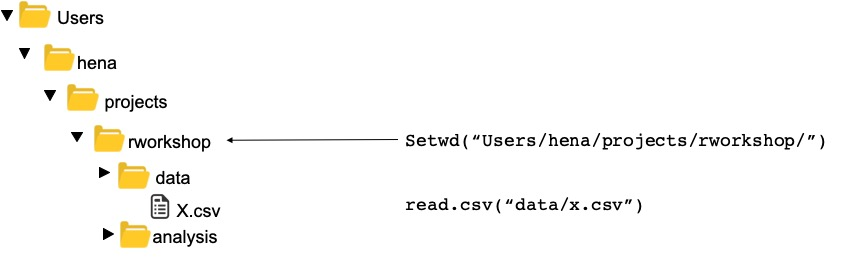
\includegraphics{filepath.jpg}

\hypertarget{how-to-learn-more}{%
\section{How to learn more?}\label{how-to-learn-more}}

The material we cover during this workshop will give you an initial taste of how you can use R to analyze data for your own research. However, you will need to learn more to do advanced operations. The best way to become proficient and efficient at R, as with any other tool, is to use it to address your actual research questions. As a beginner, it can feel daunting to have to write a script from scratch, and given that many people make their code available online, modifying existing code to suit your purpose might make it easier for you to get started.

The following part of this section is from \href{\%22https://moderndive.com/2-getting-started.html\%22}{``Modern Dive Section 2.2.3''}

Learning to code/program is very much like learning a foreign language, it can be very daunting and frustrating at first. Such frustrations are very common and it is very normal to feel discouraged as you learn. However just as with learning a foreign language, if you put in the effort and are not afraid to make mistakes, anybody can learn.

Here are a few useful tips to keep in mind as you learn to program:

\begin{itemize}
\tightlist
\item
  Remember that computers are not actually that smart: You may think your computer or smartphone are ``smart,'' but really people spent a lot of time and energy designing them to appear ``smart.'' Rather you have to tell a computer everything it needs to do. Furthermore the instructions you give your computer can't have any mistakes in them, nor can they be ambiguous in any way.
\item
  Take the ``copy, paste, and tweak'' approach: Especially when learning your first programming language, it is often much easier to taking existing code that you know works and modify it to suit your ends, rather than trying to write new code from scratch. We call this the copy, paste, and tweak approach. So early on, we suggest not trying to write code from memory, but rather take existing examples we have provided you, then copy, paste, and tweak them to suit your goals. Don't be afraid to play around!
\item
  The best way to learn to code is by doing: Rather than learning to code for its own sake, we feel that learning to code goes much smoother when you have a goal in mind or when you are working on a particular project, like analyzing data that you are interested in.
\item
  Practice is key: Just as the only method to improving your foreign language skills is through practice, practice, and practice; so also the only method to improving your coding is through practice, practice, and practice.
\end{itemize}

\hypertarget{seeking-help}{%
\subsection*{Seeking help}\label{seeking-help}}
\addcontentsline{toc}{subsection}{Seeking help}

One of the fastest ways to get help is to use the RStudio help interface. This panel by default can be found at the lower right hand panel of RStudio. As seen in the screenshot, by typing the word ``Mean'', RStudio tries to also give a number of suggestions that you might be interested in. The description is then shown in the display window.

If you need help with a specific function, let's say \texttt{barplot()}, you can type:

\begin{Shaded}
\begin{Highlighting}[]
\NormalTok{?barplot}
\end{Highlighting}
\end{Shaded}

If you just need to remind yourself of the names of the arguments, you can use:

\begin{Shaded}
\begin{Highlighting}[]
\FunctionTok{args}\NormalTok{(lm)}
\end{Highlighting}
\end{Shaded}

\begin{verbatim}
## function (formula, data, subset, weights, na.action, method = "qr", 
##     model = TRUE, x = FALSE, y = FALSE, qr = TRUE, singular.ok = TRUE, 
##     contrasts = NULL, offset, ...) 
## NULL
\end{verbatim}

If you are looking for a function to do a particular task, you can use the \texttt{help.search()} function, which is called by the double question mark ??. However, this only looks through the installed packages for help pages with a match to your search request

\begin{Shaded}
\begin{Highlighting}[]
\NormalTok{??kruskal}
\end{Highlighting}
\end{Shaded}

If you can't find what you are looking for, you can use the \href{https://www.rdocumentation.org}{rdocumentation.org} website that searches through the help files across all packages available.

\hypertarget{i-am-stuck-i-get-an-error-message-that-i-dont-understand}{%
\subsection*{I am stuck\ldots{} I get an error message that I don't understand}\label{i-am-stuck-i-get-an-error-message-that-i-dont-understand}}
\addcontentsline{toc}{subsection}{I am stuck\ldots{} I get an error message that I don't understand}

Start by googling the error message. However, this doesn't always work very well because often, package developers rely on the error catching provided by R. You end up with general error messages that might not be very helpful to diagnose a problem (e.g.~``subscript out of bounds''). If the message is very generic, you might also include the name of the function or package you're using in your query.

However, you should check Stack Overflow. Search using the \texttt{{[}r{]}} tag. Most questions have already been answered, but the challenge is to use the right words in the search to find the answers: \href{http://stackoverflow.com/questions/tagged/r}{}

\hypertarget{asking-for-help}{%
\subsection*{Asking for help}\label{asking-for-help}}
\addcontentsline{toc}{subsection}{Asking for help}

The key to receiving help from someone is for them to rapidly grasp your problem. You should make it as easy as possible to pinpoint where the issue might be.

Try to use the correct words to describe your problem. For instance, a package is not the same thing as a library. Most people will understand what you meant, but others have really strong feelings about the difference in meaning. The key point is that it can make things confusing for people trying to help you. Be as precise as possible when describing your problem.

If possible, try to reduce what doesn't work to a simple \emph{reproducible example}. If you can reproduce the problem using a very small data frame instead of your 50,000 rows and 10,000 columns one, provide the small one with the description of your problem. When appropriate, try to generalize what you are doing so even people who are not in your field can understand the question. For instance instead of using a subset of your real dataset, create a small (3 columns, 5 rows) generic one. For more information on how to write a reproducible example see \href{\%22http://adv-r.had.co.nz/Reproducibility.html\%22}{this article by Hadley Wickham}.

\hypertarget{where-to-ask-for-help}{%
\subsection*{Where to ask for help?}\label{where-to-ask-for-help}}
\addcontentsline{toc}{subsection}{Where to ask for help?}

\begin{itemize}
\tightlist
\item
  Stack Overflow: if your question hasn't been answered before and is well crafted, chances are you will get an answer in less than 5 min. Remember to follow their guidelines on how to ask a good question.
  The R-help mailing list: it is read by a lot of people (including most of the R core team), a lot of people post to it, but the tone can be pretty dry, and it is not always very welcoming to new users. If your question is valid, you are likely to get an answer very fast but don't expect that it will come with smiley faces. Also, here more than anywhere else, be sure to use correct vocabulary (otherwise you might get an answer pointing to the misuse of your words rather than answering your question). You will also have more success if your question is about a base function rather than a specific package.
\item
  The \href{https://community.rstudio.com/}{``RStudio Community''}
\item
  If your question is about a specific package, see if there is a mailing list for it. Usually it's included in the DESCRIPTION file of the package that can be accessed using packageDescription(``name-of-package''). You may also want to try to email the author of the package directly, or open an issue on the code repository (e.g., GitHub).
\end{itemize}

\hypertarget{how-to-ask-for-r-help-useful-guidelines}{%
\subsection*{How to ask for R help useful guidelines}\label{how-to-ask-for-r-help-useful-guidelines}}
\addcontentsline{toc}{subsection}{How to ask for R help useful guidelines}

\begin{itemize}
\tightlist
\item
  \href{https://blog.revolutionanalytics.com/2014/01/how-to-ask-for-r-help.html}{``How to ask for R help''} has useful guidelines
\item
  This \href{https://codeblog.jonskeet.uk/2010/08/29/writing-the-perfect-question/}{blog post by Jon Skeet} has quite comprehensive advice on how to ask programming questions.
\item
  The \href{https://cran.rstudio.com/web/packages/reprex/}{``reprex''} package is very helpful to create reproducible examples when asking for help.

  \begin{itemize}
  \tightlist
  \item
    The rOpensci blog on \href{https://ropensci.org/commcalls/2017-03-07/}{How to ask questions so they get answered} and \href{https://vimeo.com/208749032}{``video recording''} includes a presentation of the reprex package and of its philosophy.
  \end{itemize}
\end{itemize}

\hypertarget{installing-r-packages}{%
\chapter{Installing R Packages}\label{installing-r-packages}}

\hypertarget{what-are-r-packages}{%
\section{What are R packages?}\label{what-are-r-packages}}

R packages extend the functionality of R by providing additional functions, data, and documentation for specific tasks. They are written by a world-wide community of R users and can be downloaded for free from the internet. A good analogy for R packages is they are like apps you can download onto a mobile phone.

So R is like a new mobile phone: while it has a certain amount of features when you use it for the first time, it doesn't have everything. R packages are the apps you download onto your phone from Apple's App Store or Android's Google Play.

Say you have purchased a new phone and you would like to share a recent photo you have taken on Instagram. You need to:

\begin{enumerate}
\def\labelenumi{\arabic{enumi}.}
\item
  Install the app: Since your phone is new and does not include the Instagram app, you need to download the app from either the App Store or Google Play. You do this once and you're set. You might do this again in the future any time there is an update to the app.
\item
  Open the app: After you've installed Instagram, you need to open the app.
\end{enumerate}

Once Instagram is open on your phone, you can then proceed to share your photo with your friends. The process is very similar for using an R package. You need to:

\begin{enumerate}
\def\labelenumi{\arabic{enumi}.}
\tightlist
\item
  \emph{Install the package}: Most packages are not installed by default when you install R and RStudio. Thus if you want to use a package for the first time, you need to install it first. Once you've installed a package, you likely won't install it again unless you want to update it to a newer version.\\
\item
  \emph{Load the package}: Packages are not loaded by default when you start RStudio on your computer; you need to load each package you want to use every time you start RStudio.
\end{enumerate}

\hypertarget{installing-r-packages-from-different-sources}{%
\section{Installing R packages from different sources}\label{installing-r-packages-from-different-sources}}

There are multiple sources of R packages.

\hypertarget{cran}{%
\subsection*{1. CRAN}\label{cran}}
\addcontentsline{toc}{subsection}{1. CRAN}

CRAN is the ``Comprehensive R Archive Network'' - the main repository (or collection) of R packages.

There are three ways to install an R package from CRAN. For example, to install the \texttt{tidyverse} metapackage (a package of packages):

\begin{enumerate}
\def\labelenumi{\arabic{enumi}.}
\tightlist
\item
  \textbf{Easy way}: In the Files pane of RStudio:

  \begin{enumerate}
  \def\labelenumii{\alph{enumii}.}
  \tightlist
  \item
    Click on the \texttt{Packages} tab
  \item
    Click on \texttt{Install}
  \item
    Type the name of the package under ``Packages (separate multiple with space or comma):'' In this case, type \texttt{tidyverse}
  \item
    Click \texttt{Install}
  \end{enumerate}
\item
  \textbf{Easy way}: In the menu bar of RStudio:

  \begin{enumerate}
  \def\labelenumii{\alph{enumii}.}
  \tightlist
  \item
    Click on \texttt{Tools} and \texttt{Install\ Packages...}
  \item
    Type the name of the package under ``Packages (separate multiple with space or comma):'' In this case, type \texttt{tidyverse}
  \item
    Click \texttt{Install}
  \end{enumerate}
\item
  \textbf{Slightly harder way}: An alternative way to install a package is by typing \texttt{install.packages("tidyverse")} in the Console pane of RStudio and hitting enter. Note you must include the quotation marks.
\end{enumerate}

If you want to update an already installed package to a newer version, you need to re-install it by repeating the above steps.

\hypertarget{bioconductor}{%
\subsection*{2. Bioconductor}\label{bioconductor}}
\addcontentsline{toc}{subsection}{2. Bioconductor}

Bioconductor is a repository for R packages that concern computational biology or bioinformatics. To install the \texttt{knitr} package from Bioconductor, type the following in the Console of RStudio:

\begin{Shaded}
\begin{Highlighting}[]
\ControlFlowTok{if}\NormalTok{ (}\SpecialCharTok{!}\FunctionTok{requireNamespace}\NormalTok{(}\StringTok{"BiocManager"}\NormalTok{, }\AttributeTok{quietly =} \ConstantTok{TRUE}\NormalTok{))}
    \FunctionTok{install.packages}\NormalTok{(}\StringTok{"BiocManager"}\NormalTok{)}
\NormalTok{BiocManager}\SpecialCharTok{::}\FunctionTok{install}\NormalTok{(}\StringTok{"knitr"}\NormalTok{)}
\end{Highlighting}
\end{Shaded}

\hypertarget{github}{%
\subsection*{3. Github}\label{github}}
\addcontentsline{toc}{subsection}{3. Github}

Some packages are not hosted on CRAN or Bioconductor, but are instead stored in Github repositories. Sometimes this is because they are very new and have not yet been contributed. To install the \texttt{dplyr} package from Github, type the following in the Console of RStudio:

\begin{Shaded}
\begin{Highlighting}[]
\FunctionTok{install.packages}\NormalTok{(}\StringTok{"devtools"}\NormalTok{)}
\FunctionTok{library}\NormalTok{(devtools)}
\FunctionTok{install\_github}\NormalTok{(}\StringTok{"hadley/dplyr"}\NormalTok{)}
\end{Highlighting}
\end{Shaded}

\hypertarget{exercise-4.2.1}{%
\subsubsection*{EXERCISE 4.2.1}\label{exercise-4.2.1}}
\addcontentsline{toc}{subsubsection}{EXERCISE 4.2.1}

Practice what you have just learned and install the R package \texttt{ggplot2}.

\hypertarget{loading-a-package}{%
\section{Loading a package}\label{loading-a-package}}

Recall that after you've installed a package, you need to ``load'' it, in other words open it. We do this by using the \texttt{library()} command. For example, to load the \texttt{tidyverse} package, run the following code in the Console pane. What do we mean by ``run the following code''? Either type or copy \& paste the following code into the Console pane and then hit the enter key.

\begin{Shaded}
\begin{Highlighting}[]
\FunctionTok{library}\NormalTok{(tidyverse)}
\end{Highlighting}
\end{Shaded}

If after running the above code, a blinking cursor returns next to the \texttt{\textgreater{}} ``prompt'' sign, it means you were successful and the \texttt{tidyverse} package is now loaded and ready to use. If however, you get a red ``error message'' that reads\ldots{}

\begin{verbatim}
Error in library(tidyverse) : there is no package called ‘tidyverse’
\end{verbatim}

it means that you didn't successfully install it. In that case, go back to the previous subsection and trying install it again.

\hypertarget{exercise-4.3.1}{%
\subsubsection*{EXERCISE 4.3.1}\label{exercise-4.3.1}}
\addcontentsline{toc}{subsubsection}{EXERCISE 4.3.1}

Confirm that you successfully installed the packages \texttt{ggplot2}, \texttt{dplyr} and \texttt{knitr} by loading them.

\hypertarget{package-use}{%
\subsubsection*{Package use}\label{package-use}}
\addcontentsline{toc}{subsubsection}{Package use}

One extremely common mistake new R users make when wanting to use particular packages is they forget to ``load'' them first by using the \texttt{library()} command we just saw. Remember: you have to load each package you want to use every time you start RStudio. If you don't first ``load'' a package, but attempt to use one of its features, you'll see an error message similar to:

\begin{verbatim}
Error: could not find function
\end{verbatim}

R is telling you that you are trying to use a function in a package that has not yet been ``loaded''. Almost all new users forget do this when starting out, and it is a little annoying to get used to. However, you'll remember with practice.

\hypertarget{r-basics}{%
\chapter{R Basics}\label{r-basics}}

\hypertarget{creating-objects-in-r}{%
\section{Creating objects in R}\label{creating-objects-in-r}}

You can get output from R simply by typing math in the console:

\begin{Shaded}
\begin{Highlighting}[]
\DecValTok{3} \SpecialCharTok{+} \DecValTok{5}
\end{Highlighting}
\end{Shaded}

\begin{verbatim}
## [1] 8
\end{verbatim}

\begin{Shaded}
\begin{Highlighting}[]
\DecValTok{12} \SpecialCharTok{/} \DecValTok{7}
\end{Highlighting}
\end{Shaded}

\begin{verbatim}
## [1] 1.714286
\end{verbatim}

However, to do useful and interesting things, we need to assign values to objects. To create an object, we need to give it a name followed by the assignment operator \texttt{\textless{}-} or \texttt{=}, and the value we want to give it:

\begin{Shaded}
\begin{Highlighting}[]
\NormalTok{weight\_kg }\OtherTok{\textless{}{-}} \DecValTok{55}
\end{Highlighting}
\end{Shaded}

\texttt{\textless{}-} is the \emph{assignment} operator. It assigns values on the right to objects on the left. So, after executing \texttt{x\ \textless{}-\ 3}, the value of \texttt{x} is \texttt{3}. The arrow can be read as 3 \textbf{goes into} x. For historical reasons, you can also use \texttt{=} for assignments, but not in every context. Because of the slight differences in syntax, it is best practice to always use \texttt{\textless{}-} for assignments.

Objects can be given any name such as \texttt{x}, \texttt{current\_temperature}, or \texttt{subject\_id}. You want your object names to be explicit and not too long.

They cannot start with a number (\texttt{2x} is not valid, but \texttt{x2} is). R is case sensitive (e.g., \texttt{weight\_kg} is different from \texttt{Weight\_kg}).

There are some names that cannot be used because they are the names of fundamental functions in R (e.g., \texttt{if}, \texttt{else}, \texttt{for}, see \href{https://stat.ethz.ch/R-manual/R-devel/library/base/html/Reserved.html}{here} for a complete list). In general, even if it's allowed, it's best to not use other function names (e.g., \texttt{c}, \texttt{mean}, \texttt{data}, \texttt{weights}). If in doubt, check the help to see if the name is already in use. It's also best to avoid dots (\texttt{.}) within an object name as in \texttt{my.dataset}. There are many functions in R with dots in their names for historical reasons, but because dots have a special meaning in R (for methods) and other programming languages, it's best to avoid them. It is also recommended to use nouns for object names, and verbs for function names.

It's important to be consistent in the styling of your code (where you put spaces, how you name objects, etc.). Using a consistent coding style makes your code clearer to read for your future self and your collaborators. In R, three popular style guides are \href{https://google.github.io/styleguide/Rguide.xml}{Google's}, \href{\%22http://jef.works/R-style-guide/\%22}{Jean Fan's} and the \href{https://style.tidyverse.org/}{tidyverse's}.
This may seem overwhelming at first. My suggestion is to focus on what makes sense to you, and that you are using naming conventions that will help you to remember what is stored in each object. Try and be consistent with spacing and capitalization (or not) --- your future self will thank you.

\hypertarget{objects-vs.-variables}{%
\section{Objects vs.~variables}\label{objects-vs.-variables}}

What are known as \texttt{objects} in \texttt{R} are known as \texttt{variables} in many other programming languages. In this lesson, the two words are used synonymously. For more information see \url{https://cran.r-project.org/doc/manuals/r-release/R-lang.html\#Objects}

When assigning a value to an object, R does not print anything. You can force R to print the value by using parentheses or by typing the object name.

\begin{Shaded}
\begin{Highlighting}[]
\NormalTok{weight\_kg }\OtherTok{\textless{}{-}} \DecValTok{55} \CommentTok{\#  doesn\textquotesingle{}t print anything}
\end{Highlighting}
\end{Shaded}

\begin{Shaded}
\begin{Highlighting}[]
\NormalTok{(weight\_kg }\OtherTok{\textless{}{-}} \DecValTok{55}\NormalTok{) }\CommentTok{\#  will print the value of \textasciigrave{}weight\_kg\textasciigrave{}}
\end{Highlighting}
\end{Shaded}

\begin{verbatim}
## [1] 55
\end{verbatim}

\begin{Shaded}
\begin{Highlighting}[]
\NormalTok{weight\_kg         }\CommentTok{\#  and so does typing the name of the object}
\end{Highlighting}
\end{Shaded}

\begin{verbatim}
## [1] 55
\end{verbatim}

Now that R has \texttt{weight\_kg} in memory, we can do arithmetic with it. For instance, we may want to convert this weight into pounds (weight in pounds is 2.2 times the weight in kg):

\begin{Shaded}
\begin{Highlighting}[]
\FloatTok{2.2} \SpecialCharTok{*}\NormalTok{ weight\_kg}
\end{Highlighting}
\end{Shaded}

\begin{verbatim}
## [1] 121
\end{verbatim}

We can also change an object's value by assigning it a new one:

\begin{Shaded}
\begin{Highlighting}[]
\NormalTok{weight\_kg }\OtherTok{\textless{}{-}} \FloatTok{57.5}
\FloatTok{2.2} \SpecialCharTok{*}\NormalTok{ weight\_kg}
\end{Highlighting}
\end{Shaded}

\begin{verbatim}
## [1] 126.5
\end{verbatim}

This means that assigning a value to one object does not change the values of other objects For example, let's store the animal's weight in pounds in a new object, \texttt{weight\_lb}:

\begin{Shaded}
\begin{Highlighting}[]
\NormalTok{weight\_lb }\OtherTok{\textless{}{-}} \FloatTok{2.2} \SpecialCharTok{*}\NormalTok{ weight\_kg}
\end{Highlighting}
\end{Shaded}

and then change weight\_kg to 100.

\begin{Shaded}
\begin{Highlighting}[]
\NormalTok{weight\_kg }\OtherTok{\textless{}{-}} \DecValTok{100}
\end{Highlighting}
\end{Shaded}

What do you think is the current content of the object \texttt{weight\_lb}? 126.5 or 220?

\hypertarget{functions-and-their-arguments}{%
\section{Functions and their arguments}\label{functions-and-their-arguments}}

Functions are ``canned scripts'' that automate more complicated sets of commands including operations assignments, etc. Many functions are predefined, or can be made available by importing R packages.

A function usually takes one or more inputs called arguments. Functions often (but not always) return a value. A typical example would be the function \texttt{sqrt()}. The input (the argument) must be a number, and the return value (in fact, the output) is the square root of that number.

You can think of a function call generally as

\begin{verbatim}
do_this(to_that)
do_that(to_this, to_that, with_those)
\end{verbatim}

Executing a function (`running it') is called calling the function. An couple of examples of function calls are:

\begin{Shaded}
\begin{Highlighting}[]
\FunctionTok{print}\NormalTok{(}\StringTok{"hello world"}\NormalTok{)}
\end{Highlighting}
\end{Shaded}

\begin{verbatim}
## [1] "hello world"
\end{verbatim}

\begin{Shaded}
\begin{Highlighting}[]
\NormalTok{a }\OtherTok{\textless{}{-}} \DecValTok{9}
\NormalTok{b }\OtherTok{\textless{}{-}} \FunctionTok{sqrt}\NormalTok{(a)}
\NormalTok{b}
\end{Highlighting}
\end{Shaded}

\begin{verbatim}
## [1] 3
\end{verbatim}

Here, the value of \texttt{a} is given to the \texttt{sqrt()} function, the \texttt{sqrt()} function calculates the square root, and returns the value which is then assigned to the object \texttt{b}. This function is very simple, because it takes just one argument.

The return `value' of a function need not be numerical (like that of \texttt{sqrt()}), and it also does not need to be a single item: it can be a set of things, or even a dataset. We'll see that when we read data files into R.

Arguments can be anything, not only numbers or filenames, but also other objects. Exactly what each argument means differs per function, and must be looked up in the documentation (see below). Some functions take arguments which may either be specified by the user, or, if left out, take on a default value: these are called options. Options are typically used to alter the way the function operates, such as whether it ignores `bad values', or what symbol to use in a plot. However, if you want something specific, you can specify a value of your choice which will be used instead of the default.

Let's try a function that can take multiple arguments: \texttt{round()}.

\begin{Shaded}
\begin{Highlighting}[]
\FunctionTok{round}\NormalTok{(}\FloatTok{3.14159}\NormalTok{)}
\end{Highlighting}
\end{Shaded}

\begin{verbatim}
## [1] 3
\end{verbatim}

Here, we've called \texttt{round()} with just one argument, \texttt{3.14159}, and it has returned the value 3. That's because the default is to round to the nearest whole number. If we want more digits we can see how to do that by getting information about the round function. We can use \texttt{args(round)} to find what arguments it takes, or look at the help for this function using \texttt{?round}.

\begin{Shaded}
\begin{Highlighting}[]
\FunctionTok{args}\NormalTok{(round)}
\end{Highlighting}
\end{Shaded}

\begin{verbatim}
## function (x, digits = 0) 
## NULL
\end{verbatim}

\begin{Shaded}
\begin{Highlighting}[]
\NormalTok{?round}
\end{Highlighting}
\end{Shaded}

We see that if we want a different number of digits, we can type \texttt{digits\ =\ 2} or however many we want.

\begin{Shaded}
\begin{Highlighting}[]
\FunctionTok{round}\NormalTok{(}\FloatTok{3.14159}\NormalTok{, }\AttributeTok{digits =} \DecValTok{2}\NormalTok{)}
\end{Highlighting}
\end{Shaded}

\begin{verbatim}
## [1] 3.14
\end{verbatim}

If you provide the arguments in the exact same order as they are defined you don't have to name them:

\begin{Shaded}
\begin{Highlighting}[]
\FunctionTok{round}\NormalTok{(}\FloatTok{3.14159}\NormalTok{, }\DecValTok{2}\NormalTok{)}
\end{Highlighting}
\end{Shaded}

\begin{verbatim}
## [1] 3.14
\end{verbatim}

And if you do name the arguments, you can switch their order:

\begin{Shaded}
\begin{Highlighting}[]
\FunctionTok{round}\NormalTok{(}\AttributeTok{digits =} \DecValTok{2}\NormalTok{, }\AttributeTok{x =} \FloatTok{3.14159}\NormalTok{)}
\end{Highlighting}
\end{Shaded}

\begin{verbatim}
## [1] 3.14
\end{verbatim}

It's good practice to put the non-optional arguments (like the number you're rounding) first in your function call, and to then specify the names of all optional arguments. If you don't, someone reading your code might have to look up the definition of a function with unfamiliar arguments to understand what you're doing.

\hypertarget{exercise-5.3}{%
\subsubsection*{EXERCISE 5.3}\label{exercise-5.3}}
\addcontentsline{toc}{subsubsection}{EXERCISE 5.3}

Compute the golden ratio in a single line of code. One approximation of the golden ratio can be found by taking the sum of 1 and the square root of 5, and dividing by 2. Compute the golden ratio to 3 digits of precision using the \texttt{sqrt()} and \texttt{round()} functions. Hint: you can place one function inside of another.

\hypertarget{data-types-in-r}{%
\section{Data types in R}\label{data-types-in-r}}

So far we have been storing integer values in the above examples, now lets look at other data types present in R. There are several data types such as integer, string, etc. The operating system allocates memory based on the data type of the variable and decides what can be stored in the reserved memory.

There are the following data types which are used in R programming:

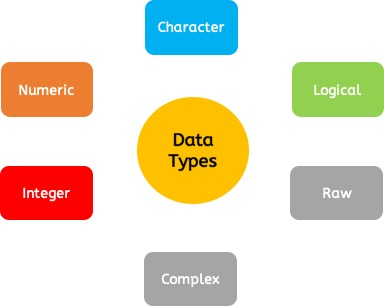
\includegraphics{datatypes.jpg}

\begin{longtable}[]{@{}
  >{\raggedright\arraybackslash}p{(\columnwidth - 4\tabcolsep) * \real{0.13}}
  >{\centering\arraybackslash}p{(\columnwidth - 4\tabcolsep) * \real{0.23}}
  >{\raggedleft\arraybackslash}p{(\columnwidth - 4\tabcolsep) * \real{0.63}}@{}}
\toprule
\begin{minipage}[b]{\linewidth}\raggedright
Data type
\end{minipage} & \begin{minipage}[b]{\linewidth}\centering
Example
\end{minipage} & \begin{minipage}[b]{\linewidth}\raggedleft
Description
\end{minipage} \\
\midrule
\endhead
\textbf{Logical} & True, False & It is a special data type for data with only two possible values which can be construed as true/false. \\
\textbf{Numeric} & 12,32,112,5432 & Decimal value is called numeric in R, and it is the default computational data type. \\
\textbf{Integer} & 3L, 66L, 2346L & Here, L tells R to store the value as an integer, \\
\textbf{Complex} & Z=1+2i, t=7+3i & A complex value in R is defined as the pure imaginary value i. \\
\textbf{Character} & `a', `\,``good''', ``TRUE'', '35.4' & In R programming, a character is used to represent string values. We convert objects into character values with the help ofas.character() function. \\
\textbf{Raw} & & A raw data type is used to holds raw bytes. \\
\bottomrule
\end{longtable}

\begin{Shaded}
\begin{Highlighting}[]
\NormalTok{weight\_kg }\OtherTok{\textless{}{-}} \DecValTok{100}
\NormalTok{name}\OtherTok{\textless{}{-}}\StringTok{"Samantha"}
\NormalTok{present}\OtherTok{\textless{}{-}}\ConstantTok{TRUE}
\end{Highlighting}
\end{Shaded}

\hypertarget{data-structures-in-r}{%
\section{Data structures in R}\label{data-structures-in-r}}

R has six types of basic data structures. We can organize these data structures according to their dimensions(1d, 2d, nd). We can also classify them as homogeneous or heterogeneous (can their contents be of different datatypes or not).

Homogeneous data structures are ones that can only store a single type of data (numeric, integer, character, etc.).

Heterogeneous data structures are ones that can store more than one type of data at the same time.

R does not have 0 dimensional or scalar type. Variables containing single values are vectors of length 1.

R has the following basic data structures:

\begin{enumerate}
\def\labelenumi{\arabic{enumi}.}
\tightlist
\item
  Vector (1d,homegenous)
\item
  List (heterogeneous)
\item
  Matrix (2d, homogeneous)
\item
  Data frame (tibble) (2d, heterogeneous)
\item
  Array (3d,homogeneous)
\end{enumerate}

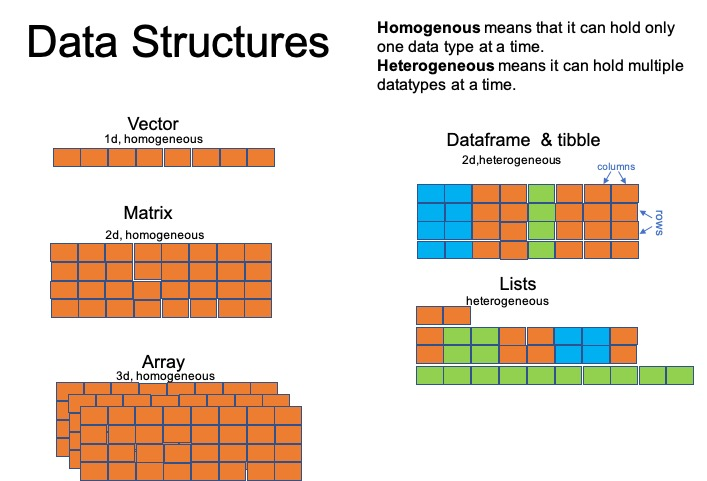
\includegraphics{data_s.jpg}

\hypertarget{exercise-5.5}{%
\subsubsection*{EXERCISE 5.5}\label{exercise-5.5}}
\addcontentsline{toc}{subsubsection}{EXERCISE 5.5}

In which data sturctures can we put multiple data types?

\hypertarget{vectors}{%
\section{Vectors}\label{vectors}}

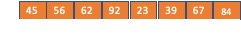
\includegraphics{vec1.jpg}

A vector is the most common and basic data type in R, and is pretty much the workhorse of R. A vector is a collection of values that are all of the same type (numeric, character, etc.). We can assign a series of values to a vector using the \texttt{c()} function. For example we can create a vector of animal weights and assign it to a new object \texttt{weight\_g}:

\begin{Shaded}
\begin{Highlighting}[]
\NormalTok{weight\_g }\OtherTok{\textless{}{-}} \FunctionTok{c}\NormalTok{(}\DecValTok{50}\NormalTok{, }\DecValTok{60}\NormalTok{, }\DecValTok{65}\NormalTok{, }\DecValTok{82}\NormalTok{)}
\NormalTok{weight\_g}
\end{Highlighting}
\end{Shaded}

\begin{verbatim}
## [1] 50 60 65 82
\end{verbatim}

A vector can also contain characters:

\begin{Shaded}
\begin{Highlighting}[]
\NormalTok{animals }\OtherTok{\textless{}{-}} \FunctionTok{c}\NormalTok{(}\StringTok{"mouse"}\NormalTok{, }\StringTok{"rat"}\NormalTok{, }\StringTok{"dog"}\NormalTok{)}
\NormalTok{animals}
\end{Highlighting}
\end{Shaded}

\begin{verbatim}
## [1] "mouse" "rat"   "dog"
\end{verbatim}

The quotes around ``mouse'', ``rat'', etc. are essential here. Without the quotes R will assume objects have been created called \texttt{mouse}, \texttt{rat} and \texttt{dog}. As these objects don't exist in R's memory, there will be an error message.

There are many functions that allow you to inspect the content of a vector. \texttt{length()} tells you how many elements are in a particular vector:

\begin{Shaded}
\begin{Highlighting}[]
\FunctionTok{length}\NormalTok{(weight\_g)}
\end{Highlighting}
\end{Shaded}

\begin{verbatim}
## [1] 4
\end{verbatim}

\begin{Shaded}
\begin{Highlighting}[]
\FunctionTok{length}\NormalTok{(animals)}
\end{Highlighting}
\end{Shaded}

\begin{verbatim}
## [1] 3
\end{verbatim}

An important feature of a vector, is that all of the elements are the same type of data. The function \texttt{class()} indicates the class (the type of element) of an object:

\begin{Shaded}
\begin{Highlighting}[]
\FunctionTok{class}\NormalTok{(weight\_g)}
\end{Highlighting}
\end{Shaded}

\begin{verbatim}
## [1] "numeric"
\end{verbatim}

\begin{Shaded}
\begin{Highlighting}[]
\FunctionTok{class}\NormalTok{(animals)}
\end{Highlighting}
\end{Shaded}

\begin{verbatim}
## [1] "character"
\end{verbatim}

The function \texttt{str()} provides an overview of the structure of an object and its elements. It is a useful function when working with large and complex objects:

\begin{Shaded}
\begin{Highlighting}[]
\FunctionTok{str}\NormalTok{(weight\_g)}
\end{Highlighting}
\end{Shaded}

\begin{verbatim}
##  num [1:4] 50 60 65 82
\end{verbatim}

\begin{Shaded}
\begin{Highlighting}[]
\FunctionTok{str}\NormalTok{(animals)}
\end{Highlighting}
\end{Shaded}

\begin{verbatim}
##  chr [1:3] "mouse" "rat" "dog"
\end{verbatim}

You can use the \texttt{c()} function to add other elements to your vector:

\begin{Shaded}
\begin{Highlighting}[]
\NormalTok{weight\_g }\OtherTok{\textless{}{-}} \FunctionTok{c}\NormalTok{(weight\_g, }\DecValTok{90}\NormalTok{) }\CommentTok{\# add to the end of the vector}
\NormalTok{weight\_g }\OtherTok{\textless{}{-}} \FunctionTok{c}\NormalTok{(}\DecValTok{30}\NormalTok{, weight\_g) }\CommentTok{\# add to the beginning of the vector}
\NormalTok{weight\_g}
\end{Highlighting}
\end{Shaded}

\begin{verbatim}
## [1] 30 50 60 65 82 90
\end{verbatim}

In the first line, we take the original vector \texttt{weight\_g}, add the value 90 to the end of it, and save the result back into \texttt{weight\_g}. Then we add the value \texttt{30} to the beginning, again saving the result back into \texttt{weight\_g}.

We can do this over and over again to grow a vector, or assemble a dataset. As we program, this may be useful to add results that we are collecting or calculating.

\hypertarget{indexing-vectors}{%
\section{Indexing vectors}\label{indexing-vectors}}

If we want to extract one or several values from a vector, we must provide one or several indices in square brackets. For instance:

\begin{Shaded}
\begin{Highlighting}[]
\NormalTok{animals }\OtherTok{\textless{}{-}} \FunctionTok{c}\NormalTok{(}\StringTok{"mouse"}\NormalTok{, }\StringTok{"rat"}\NormalTok{, }\StringTok{"dog"}\NormalTok{, }\StringTok{"cat"}\NormalTok{)}
\CommentTok{\# Get the 2nd value in the animals vector}
\NormalTok{animals[}\DecValTok{2}\NormalTok{]}
\end{Highlighting}
\end{Shaded}

\begin{verbatim}
## [1] "rat"
\end{verbatim}

\begin{Shaded}
\begin{Highlighting}[]
\CommentTok{\# Get the 1st through 3rd value in the animals vector}
\NormalTok{animals[}\DecValTok{1}\SpecialCharTok{:}\DecValTok{3}\NormalTok{]}
\end{Highlighting}
\end{Shaded}

\begin{verbatim}
## [1] "mouse" "rat"   "dog"
\end{verbatim}

\begin{Shaded}
\begin{Highlighting}[]
\CommentTok{\# Get the 2nd and 4th values}
\NormalTok{animals[}\FunctionTok{c}\NormalTok{(}\DecValTok{2}\NormalTok{,}\DecValTok{4}\NormalTok{)]}
\end{Highlighting}
\end{Shaded}

\begin{verbatim}
## [1] "rat" "cat"
\end{verbatim}

R indices start at 1. Programming languages like Fortran, MATLAB, Julia, and R start counting at 1, because that's what human beings typically do. Languages in the C family (including C++, Java, Perl, and Python) count from 0 because \emph{reasons}.

\hypertarget{adding-values-to-vectors}{%
\subsection*{Adding values to vectors}\label{adding-values-to-vectors}}
\addcontentsline{toc}{subsection}{Adding values to vectors}

We can add new items to a vector using the \texttt{c()} function.

\begin{Shaded}
\begin{Highlighting}[]
\NormalTok{animals }\OtherTok{\textless{}{-}} \FunctionTok{c}\NormalTok{(animals, }\StringTok{"horse"}\NormalTok{, }\StringTok{"crab"}\NormalTok{, }\StringTok{"monkey"}\NormalTok{)}
\NormalTok{animals}
\end{Highlighting}
\end{Shaded}

\begin{verbatim}
## [1] "mouse"  "rat"    "dog"    "cat"    "horse"  "crab"   "monkey"
\end{verbatim}

\hypertarget{replacing-values-in-existing-vectors}{%
\subsection*{Replacing values in existing vectors}\label{replacing-values-in-existing-vectors}}
\addcontentsline{toc}{subsection}{Replacing values in existing vectors}

We can replace a value by using the index of the item to be replaced:

\begin{Shaded}
\begin{Highlighting}[]
\CommentTok{\# Change monkey to bird}
\NormalTok{animals[}\DecValTok{7}\NormalTok{] }\OtherTok{\textless{}{-}} \StringTok{"bird"}
\NormalTok{animals}
\end{Highlighting}
\end{Shaded}

\begin{verbatim}
## [1] "mouse" "rat"   "dog"   "cat"   "horse" "crab"  "bird"
\end{verbatim}

\hypertarget{conditional-subsetting}{%
\section{Conditional subsetting}\label{conditional-subsetting}}

Another common way of subsetting is by using a logical vector. \texttt{TRUE} will select the element with the same index, while \texttt{FALSE} will not:

\begin{Shaded}
\begin{Highlighting}[]
\NormalTok{weight\_g }\OtherTok{\textless{}{-}} \FunctionTok{c}\NormalTok{(}\DecValTok{21}\NormalTok{, }\DecValTok{34}\NormalTok{, }\DecValTok{39}\NormalTok{, }\DecValTok{54}\NormalTok{, }\DecValTok{55}\NormalTok{)}
\NormalTok{weight\_g[}\FunctionTok{c}\NormalTok{(}\ConstantTok{TRUE}\NormalTok{, }\ConstantTok{FALSE}\NormalTok{, }\ConstantTok{TRUE}\NormalTok{, }\ConstantTok{TRUE}\NormalTok{, }\ConstantTok{FALSE}\NormalTok{)]}
\end{Highlighting}
\end{Shaded}

\begin{verbatim}
## [1] 21 39 54
\end{verbatim}

Typically, these logical vectors are not typed by hand, but are the output of other functions or logical tests. For instance, if you wanted to select only the values above 50:

\begin{Shaded}
\begin{Highlighting}[]
\NormalTok{weight\_g }\SpecialCharTok{\textgreater{}} \DecValTok{50}    \CommentTok{\# will return logicals with TRUE for the indices that meet the condition}
\end{Highlighting}
\end{Shaded}

\begin{verbatim}
## [1] FALSE FALSE FALSE  TRUE  TRUE
\end{verbatim}

\begin{Shaded}
\begin{Highlighting}[]
\DocumentationTok{\#\# so we can use this to select only the values above 50}
\NormalTok{weight\_g[weight\_g }\SpecialCharTok{\textgreater{}} \DecValTok{50}\NormalTok{]}
\end{Highlighting}
\end{Shaded}

\begin{verbatim}
## [1] 54 55
\end{verbatim}

You can combine multiple tests using \& (both conditions are true, AND) or \textbar{} (at least one of the conditions is true, OR):

\begin{Shaded}
\begin{Highlighting}[]
\NormalTok{weight\_g[weight\_g }\SpecialCharTok{\textless{}} \DecValTok{30} \SpecialCharTok{|}\NormalTok{ weight\_g }\SpecialCharTok{\textgreater{}} \DecValTok{50}\NormalTok{]}
\end{Highlighting}
\end{Shaded}

\begin{verbatim}
## [1] 21 54 55
\end{verbatim}

\begin{Shaded}
\begin{Highlighting}[]
\NormalTok{weight\_g[weight\_g }\SpecialCharTok{\textgreater{}=} \DecValTok{30} \SpecialCharTok{\&}\NormalTok{ weight\_g }\SpecialCharTok{==} \DecValTok{21}\NormalTok{]}
\end{Highlighting}
\end{Shaded}

\begin{verbatim}
## numeric(0)
\end{verbatim}

Here, \texttt{\textless{}} stands for ``less than'', \texttt{\textgreater{}} for ``greater than'', \texttt{\textgreater{}=} for ``greater than or equal to'', and \texttt{==} for ``equal to''. The double equal sign \texttt{==} is a test for numerical equality between the left and right hand sides, and should not be confused with the single \texttt{=} sign, which performs variable assignment (similar to \texttt{\textless{}-}).

\begin{longtable}[]{@{}ll@{}}
\toprule
Operator & Description \\
\midrule
\endhead
\texttt{\textless{}} & less than \\
\texttt{\textless{}=} & less than or equal to \\
\texttt{\textgreater{}} & greater than \\
\texttt{\textgreater{}=} & greater than or equal to \\
\texttt{==} & equal to \\
\texttt{!=} & not equal to \\
\texttt{!x} & not x \\
\texttt{a\textbar{}b} & a or b \\
\texttt{a\&b} & a and b \\
\bottomrule
\end{longtable}

A common task is to search for certain strings in a vector. One could use the ``or'' operator \textbar{} to test for equality to multiple values, but this can quickly become tedious. The function \texttt{\%in\%} allows you to test if any of the elements of a search vector are found:

\begin{Shaded}
\begin{Highlighting}[]
\NormalTok{animals }\OtherTok{\textless{}{-}} \FunctionTok{c}\NormalTok{(}\StringTok{"mouse"}\NormalTok{, }\StringTok{"rat"}\NormalTok{, }\StringTok{"dog"}\NormalTok{, }\StringTok{"cat"}\NormalTok{)}
\NormalTok{animals[animals }\SpecialCharTok{==} \StringTok{"cat"} \SpecialCharTok{|}\NormalTok{ animals }\SpecialCharTok{==} \StringTok{"rat"}\NormalTok{] }\CommentTok{\# returns both rat and cat}
\end{Highlighting}
\end{Shaded}

\begin{verbatim}
## [1] "rat" "cat"
\end{verbatim}

\begin{Shaded}
\begin{Highlighting}[]
\NormalTok{animals }\SpecialCharTok{\%in\%} \FunctionTok{c}\NormalTok{(}\StringTok{"rat"}\NormalTok{, }\StringTok{"cat"}\NormalTok{, }\StringTok{"dog"}\NormalTok{, }\StringTok{"duck"}\NormalTok{, }\StringTok{"goat"}\NormalTok{)}
\end{Highlighting}
\end{Shaded}

\begin{verbatim}
## [1] FALSE  TRUE  TRUE  TRUE
\end{verbatim}

\begin{Shaded}
\begin{Highlighting}[]
\NormalTok{animals[animals }\SpecialCharTok{\%in\%} \FunctionTok{c}\NormalTok{(}\StringTok{"rat"}\NormalTok{, }\StringTok{"cat"}\NormalTok{, }\StringTok{"dog"}\NormalTok{, }\StringTok{"duck"}\NormalTok{, }\StringTok{"goat"}\NormalTok{)]}
\end{Highlighting}
\end{Shaded}

\begin{verbatim}
## [1] "rat" "dog" "cat"
\end{verbatim}

The \texttt{which()} function returns the indices of any item that evaluates as TRUE in our comparison:

\begin{Shaded}
\begin{Highlighting}[]
\FunctionTok{which}\NormalTok{(animals }\SpecialCharTok{==} \StringTok{"cat"}\NormalTok{)}
\end{Highlighting}
\end{Shaded}

\begin{verbatim}
## [1] 4
\end{verbatim}

\hypertarget{exercise-5.7.1}{%
\subsubsection*{EXERCISE 5.7.1}\label{exercise-5.7.1}}
\addcontentsline{toc}{subsubsection}{EXERCISE 5.7.1}

\begin{itemize}
\tightlist
\item
  Can you figure out why ``four'' \textgreater{} ``five'' returns TRUE?
\end{itemize}

\hypertarget{missing-data}{%
\section{Missing data}\label{missing-data}}

As R was designed to analyze datasets, it includes the concept of missing data (which is uncommon in other programming languages). Missing data are represented in vectors as \texttt{NA}.

When doing operations on numbers, most functions will return \texttt{NA} if the data you are working with include missing values. This feature makes it harder to overlook the cases where you are dealing with missing data. You can add the argument na.rm = TRUE to calculate the result while ignoring the missing values.

\begin{Shaded}
\begin{Highlighting}[]
\NormalTok{heights }\OtherTok{\textless{}{-}} \FunctionTok{c}\NormalTok{(}\DecValTok{2}\NormalTok{, }\DecValTok{4}\NormalTok{, }\DecValTok{4}\NormalTok{, }\ConstantTok{NA}\NormalTok{, }\DecValTok{6}\NormalTok{)}
\FunctionTok{mean}\NormalTok{(heights)}
\end{Highlighting}
\end{Shaded}

\begin{verbatim}
## [1] NA
\end{verbatim}

\begin{Shaded}
\begin{Highlighting}[]
\FunctionTok{max}\NormalTok{(heights)}
\end{Highlighting}
\end{Shaded}

\begin{verbatim}
## [1] NA
\end{verbatim}

\begin{Shaded}
\begin{Highlighting}[]
\FunctionTok{mean}\NormalTok{(heights, }\AttributeTok{na.rm =} \ConstantTok{TRUE}\NormalTok{)}
\end{Highlighting}
\end{Shaded}

\begin{verbatim}
## [1] 4
\end{verbatim}

\begin{Shaded}
\begin{Highlighting}[]
\FunctionTok{max}\NormalTok{(heights, }\AttributeTok{na.rm =} \ConstantTok{TRUE}\NormalTok{)}
\end{Highlighting}
\end{Shaded}

\begin{verbatim}
## [1] 6
\end{verbatim}

If your data include missing values (and that's probably all of us!), you may want to become familiar with the functions \texttt{is.na()}, and \texttt{na.omit()}. See below for examples.

\begin{Shaded}
\begin{Highlighting}[]
\CommentTok{\# Extract those elements which are not missing values.}
\NormalTok{heights[}\SpecialCharTok{!}\FunctionTok{is.na}\NormalTok{(heights)]}
\end{Highlighting}
\end{Shaded}

\begin{verbatim}
## [1] 2 4 4 6
\end{verbatim}

\begin{Shaded}
\begin{Highlighting}[]
\CommentTok{\# Returns the object with incomplete cases removed.}
\FunctionTok{na.omit}\NormalTok{(heights)}
\end{Highlighting}
\end{Shaded}

\begin{verbatim}
## [1] 2 4 4 6
## attr(,"na.action")
## [1] 4
## attr(,"class")
## [1] "omit"
\end{verbatim}

\hypertarget{exercise-5.8.1}{%
\subsubsection*{EXERCISE 5.8.1}\label{exercise-5.8.1}}
\addcontentsline{toc}{subsubsection}{EXERCISE 5.8.1}

\begin{enumerate}
\def\labelenumi{\arabic{enumi}.}
\tightlist
\item
  Using this vector of heights in inches, create a new vector, \texttt{heights\_no\_na}, with the NAs removed.
\end{enumerate}

\begin{Shaded}
\begin{Highlighting}[]
\NormalTok{heights }\OtherTok{\textless{}{-}} \FunctionTok{c}\NormalTok{(}\DecValTok{63}\NormalTok{, }\DecValTok{69}\NormalTok{, }\DecValTok{60}\NormalTok{, }\DecValTok{65}\NormalTok{, }\ConstantTok{NA}\NormalTok{, }\DecValTok{68}\NormalTok{, }\DecValTok{61}\NormalTok{, }\DecValTok{70}\NormalTok{, }\DecValTok{61}\NormalTok{, }\DecValTok{59}\NormalTok{, }\DecValTok{64}\NormalTok{, }\DecValTok{69}\NormalTok{, }\DecValTok{63}\NormalTok{, }\DecValTok{63}\NormalTok{, }\ConstantTok{NA}\NormalTok{, }\DecValTok{72}\NormalTok{, }\DecValTok{65}\NormalTok{, }\DecValTok{64}\NormalTok{, }\DecValTok{70}\NormalTok{, }\DecValTok{63}\NormalTok{, }\DecValTok{65}\NormalTok{)}
\end{Highlighting}
\end{Shaded}

\begin{enumerate}
\def\labelenumi{\arabic{enumi}.}
\setcounter{enumi}{1}
\tightlist
\item
  Use the function median() to calculate the median of the heights vector.
\item
  Use R to figure out how many people in the set are taller than 67 inches.
\end{enumerate}

\hypertarget{starting-with-data}{%
\chapter{Starting with Data}\label{starting-with-data}}

\hypertarget{download-the-data}{%
\section{Download the data}\label{download-the-data}}

Make a new RStudio Project and create a \texttt{data} directory in your RStudio Project.

You can download the file directly from dropbox using \href{https://www.dropbox.com/s/gt05aqpmohd9un6/Ecoli_metadata.csv?dl=0}{this link}. Remember to put this file in a directory that makes sense (ex. in your RStudio Project directory in a \texttt{data} directory).

\hypertarget{csv-files}{%
\section{CSV files}\label{csv-files}}

Spreadsheet data is often saved in one of the following formats:

\begin{itemize}
\tightlist
\item
  A \emph{Comma Separated Values} \texttt{.csv} file. You can think of a \texttt{.csv} file as a bare-bones spreadsheet where:

  \begin{itemize}
  \tightlist
  \item
    Each line in the file corresponds to one row of data/one observation.\\
  \item
    Values for each line are separated with commas. In other words, the values of different variables are separated by commas.\\
  \item
    The first line is often, but not always, a header row indicating the names of the columns/variables.\\
  \end{itemize}
\item
  An Excel \texttt{.xlsx} file. This format is based on Microsoft's proprietary Excel software. As opposed to a bare-bones \texttt{.csv} files, \texttt{.xlsx} Excel files sometimes contain a lot of meta-data, or put more simply, data about the data. Some examples of spreadsheet meta-data include the use of bold and italic fonts, colored cells, different column widths, and formula macros.\\
\item
  A Google Sheets file, which is a ``cloud'' or online-based way to work with a spreadsheet. Google Sheets allows you to download your data in both comma separated values \texttt{.csv} and Excel \texttt{.xlsx} formats however: go to the Google Sheets menu bar -\textgreater{} File -\textgreater{} Download as -\textgreater{} Select ``Microsoft Excel'' or ``Comma-separated values.''
\end{itemize}

There are several ways to import data into R. Here, we will use the tools every R installation comes with (ie. ``base R'') to import a comma-delimited file containing some data. We will need to load the file using a function called \texttt{read.csv()}.

\hypertarget{exercise-6.2.1}{%
\subsubsection*{EXERCISE 6.2.1}\label{exercise-6.2.1}}
\addcontentsline{toc}{subsubsection}{EXERCISE 6.2.1}

Before using the \texttt{read.csv()} function, use R's help feature to answer the following questions:

\begin{enumerate}
\def\labelenumi{\arabic{enumi}.}
\tightlist
\item
  What is the default parameter for `header' in the read.csv() function?
\item
  What argument would you have to change to read a file that was delimited by semicolons (;) rather than commas?
\item
  What argument would you have to change to read file in which numbers used commas for decimal separation (i.e.~1,00)?
\item
  What argument would you have to change to read in only the first 10,000 rows of a very large file?
\end{enumerate}

\hypertarget{sidenote-importing-data-from-excel}{%
\section{Sidenote: Importing data from Excel}\label{sidenote-importing-data-from-excel}}

Excel is one of the most common formats, so we need to discuss how to make these files play nicely with R. The simplest way to import data from Excel is to save your Excel file in .csv format. You can then import into R right away. Sometimes you may not be able to do this (imagine you have data in 300 Excel files, are you going to open and export all of them?).

One common R package (a set of code with features you can download and add to your R installation) is the readxl package which can open and import Excel files.

\hypertarget{import-data}{%
\section{Import data}\label{import-data}}

Now let's read in some data. We're going to study a population of \emph{Escherichia coli} (designated Ara-3), which were propagated for more than 40,000 generations in a glucose-limited minimal medium. This medium was supplemented with citrate, which the ancestral \emph{E. coli} cannot metabolize in the aerobic conditions of the experiment. Sequencing of the populations at regular time points revealed that spontaneous citrate-using mutants (Cit+) appeared at around 31,000 generations in one of twelve populations. The dataset is stored as a comma separated value (CSV) file. This metadata describes information on the Ara-3 clones and the columns represent:

\begin{longtable}[]{@{}ll@{}}
\toprule
Column & Description \\
\midrule
\endhead
sample & clone name \\
generation & generation when sample frozen \\
clade & based on a parsimony tree \\
strain & ancestral strain \\
cit & citrate-using mutant status \\
run & sequence read archive sample ID \\
genome\_size & size in Mbp \\
\bottomrule
\end{longtable}

Read in the metadata file:

\begin{Shaded}
\begin{Highlighting}[]
\NormalTok{metadata }\OtherTok{\textless{}{-}} \FunctionTok{read.csv}\NormalTok{(}\StringTok{"data/Ecoli\_metadata.csv"}\NormalTok{)}
\end{Highlighting}
\end{Shaded}

This statement doesn't produce any output because assignment doesn't display anything. If we want to check that our data has been loaded, we can print the variable's value: \texttt{metadata}.

This will output the entire dataset. If we only want to see the top 6 lines of the file to ensure it has been loaded, use the \texttt{head()} function:

\begin{Shaded}
\begin{Highlighting}[]
\FunctionTok{head}\NormalTok{(metadata)}
\end{Highlighting}
\end{Shaded}

\begin{verbatim}
##     sample generation   clade strain     cit       run genome_size
## 1   REL606          0     N/A REL606 unknown                  4.62
## 2 REL1166A       2000 unknown REL606 unknown SRR098028        4.63
## 3   ZDB409       5000 unknown REL606 unknown SRR098281        4.60
## 4   ZDB429      10000      UC REL606 unknown SRR098282        4.59
## 5   ZDB446      15000      UC REL606 unknown SRR098283        4.66
## 6   ZDB458      20000 (C1,C2) REL606 unknown SRR098284        4.63
\end{verbatim}

\hypertarget{what-are-data-frames}{%
\section{What are data frames?}\label{what-are-data-frames}}

A data frame is the standard way in R to store tabular data. It can also be thought of as a collection of vectors, all of which have the same length. Each vector represents a column and each vector can be a different data type (ex. characters, integers).

The \texttt{str()} function is useful to insepct the data types of the columns.

\begin{Shaded}
\begin{Highlighting}[]
\FunctionTok{str}\NormalTok{(metadata)}
\end{Highlighting}
\end{Shaded}

\begin{verbatim}
## 'data.frame':    30 obs. of  7 variables:
##  $ sample     : chr  "REL606" "REL1166A" "ZDB409" "ZDB429" ...
##  $ generation : int  0 2000 5000 10000 15000 20000 20000 20000 25000 25000 ...
##  $ clade      : chr  "N/A" "unknown" "unknown" "UC" ...
##  $ strain     : chr  "REL606" "REL606" "REL606" "REL606" ...
##  $ cit        : chr  "unknown" "unknown" "unknown" "unknown" ...
##  $ run        : chr  "" "SRR098028" "SRR098281" "SRR098282" ...
##  $ genome_size: num  4.62 4.63 4.6 4.59 4.66 4.63 4.62 4.61 4.65 4.59 ...
\end{verbatim}

\hypertarget{exercise-6.5.1}{%
\subsubsection*{EXERCISE 6.5.1}\label{exercise-6.5.1}}
\addcontentsline{toc}{subsubsection}{EXERCISE 6.5.1}

Create a data frame using the \texttt{data.frame()} function:

\begin{Shaded}
\begin{Highlighting}[]
\CommentTok{\# Create the data frame}
\NormalTok{BMI }\OtherTok{\textless{}{-}} \FunctionTok{data.frame}\NormalTok{(}\AttributeTok{gender =} \FunctionTok{c}\NormalTok{(}\StringTok{"male"}\NormalTok{, }\StringTok{"male"}\NormalTok{, }\StringTok{"female"}\NormalTok{), }\AttributeTok{height =} \FunctionTok{c}\NormalTok{(}\DecValTok{152}\NormalTok{, }\FloatTok{171.5}\NormalTok{, }\DecValTok{165}\NormalTok{), }\AttributeTok{weight =} \FunctionTok{c}\NormalTok{(}\DecValTok{81}\NormalTok{, }\DecValTok{93}\NormalTok{, }\DecValTok{78}\NormalTok{), }\AttributeTok{age =} \FunctionTok{c}\NormalTok{(}\DecValTok{42}\NormalTok{, }\DecValTok{36}\NormalTok{, }\DecValTok{26}\NormalTok{))}
\CommentTok{\# Pring the data frame}
\NormalTok{BMI}
\end{Highlighting}
\end{Shaded}

\begin{verbatim}
##   gender height weight age
## 1   male  152.0     81  42
## 2   male  171.5     93  36
## 3 female  165.0     78  26
\end{verbatim}

Try the following functions on the BMI data frame:

\begin{itemize}
\tightlist
\item
  \texttt{dim()}
\item
  \texttt{nrow()}
\item
  \texttt{ncol()}
\item
  \texttt{summary()}
\item
  \texttt{rownames()}
\item
  \texttt{colnames()}
\end{itemize}

What information does each of these functions tell you?

\hypertarget{saving-or-writing-a-data-frame}{%
\subsection*{Saving or ``writing'' a data frame}\label{saving-or-writing-a-data-frame}}
\addcontentsline{toc}{subsection}{Saving or ``writing'' a data frame}

We can save a data frame to a csv file using the \texttt{write.csv()} function. For example, to save the BMI data to bmi.csv:

\begin{Shaded}
\begin{Highlighting}[]
\FunctionTok{write.csv}\NormalTok{(BMI, }\AttributeTok{file =} \StringTok{"bmi.csv"}\NormalTok{)}
\end{Highlighting}
\end{Shaded}

Ensure that you have successfully saved this csv file, then feel free to delete it.

\hypertarget{what-are-factors}{%
\section{What are factors?}\label{what-are-factors}}

Factors are the final major data structure we will introduce. Factors can be thought of as vectors which are specialized for categorical data. Given R's specialization for statistics, this make sense since categorial and continuous variables usually have different treatments. Sometimes you may want to have data treated as a factor, but in other cases, this may be undesirable.

Factors are stored as integers, and have labels associated with these unique integers. While factors look (and often behave) like character vectors, they are actually integers under the hood, and you need to be careful when treating them like strings.

\begin{Shaded}
\begin{Highlighting}[]
\FunctionTok{str}\NormalTok{(metadata)}
\end{Highlighting}
\end{Shaded}

\begin{verbatim}
## 'data.frame':    30 obs. of  7 variables:
##  $ sample     : chr  "REL606" "REL1166A" "ZDB409" "ZDB429" ...
##  $ generation : int  0 2000 5000 10000 15000 20000 20000 20000 25000 25000 ...
##  $ clade      : chr  "N/A" "unknown" "unknown" "UC" ...
##  $ strain     : chr  "REL606" "REL606" "REL606" "REL606" ...
##  $ cit        : chr  "unknown" "unknown" "unknown" "unknown" ...
##  $ run        : chr  "" "SRR098028" "SRR098281" "SRR098282" ...
##  $ genome_size: num  4.62 4.63 4.6 4.59 4.66 4.63 4.62 4.61 4.65 4.59 ...
\end{verbatim}

Here we can see which columns/variables are factors. When we read in a file, any column that contains text is automatically assumed to be a factor. Once created, factors can only contain a pre-defined set values, known as levels. By default, R always sorts levels in alphabetical order.

For instance, we see that \texttt{cit} is a Factor w/ 3 levels, \texttt{"minus"}, \texttt{"plus"} and \texttt{"unknown"}.

\hypertarget{the-sign}{%
\subsection*{The \$ sign}\label{the-sign}}
\addcontentsline{toc}{subsection}{The \$ sign}

To isolate a column or variable of a data frame, we use the \textbf{\$} operator. This applies to any type of variable. For example:

\begin{Shaded}
\begin{Highlighting}[]
\NormalTok{metadata}\SpecialCharTok{$}\NormalTok{sample}
\end{Highlighting}
\end{Shaded}

\begin{verbatim}
##  [1] "REL606"   "REL1166A" "ZDB409"   "ZDB429"   "ZDB446"   "ZDB458"  
##  [7] "ZDB464*"  "ZDB467"   "ZDB477"   "ZDB483"   "ZDB16"    "ZDB357"  
## [13] "ZDB199*"  "ZDB200"   "ZDB564"   "ZDB30*"   "ZDB172"   "ZDB158"  
## [19] "ZDB143"   "CZB199"   "CZB152"   "CZB154"   "ZDB83"    "ZDB87"   
## [25] "ZDB96"    "ZDB99"    "ZDB107"   "ZDB111"   "REL10979" "REL10988"
\end{verbatim}

\begin{Shaded}
\begin{Highlighting}[]
\NormalTok{metadata}\SpecialCharTok{$}\NormalTok{genome\_size}
\end{Highlighting}
\end{Shaded}

\begin{verbatim}
##  [1] 4.62 4.63 4.60 4.59 4.66 4.63 4.62 4.61 4.65 4.59 4.61 4.62 4.62 4.63 4.74
## [16] 4.61 4.77 4.63 4.79 4.59 4.80 4.76 4.60 4.75 4.74 4.61 4.79 4.62 4.78 4.62
\end{verbatim}

To determine the number of levels of any factor, use the \texttt{nlevels()} function:

\begin{Shaded}
\begin{Highlighting}[]
\FunctionTok{nlevels}\NormalTok{(metadata}\SpecialCharTok{$}\NormalTok{run)}
\end{Highlighting}
\end{Shaded}

\begin{verbatim}
## [1] 0
\end{verbatim}

\begin{Shaded}
\begin{Highlighting}[]
\FunctionTok{nlevels}\NormalTok{(metadata}\SpecialCharTok{$}\NormalTok{clade)}
\end{Highlighting}
\end{Shaded}

\begin{verbatim}
## [1] 0
\end{verbatim}

\begin{Shaded}
\begin{Highlighting}[]
\FunctionTok{nlevels}\NormalTok{(metadata}\SpecialCharTok{$}\NormalTok{strain)}
\end{Highlighting}
\end{Shaded}

\begin{verbatim}
## [1] 0
\end{verbatim}

Let's extract the \texttt{cit} column of the metadata to a new object, so we don't end up modifying our original data frame.

\begin{Shaded}
\begin{Highlighting}[]
\NormalTok{cit }\OtherTok{\textless{}{-}}\NormalTok{ metadata}\SpecialCharTok{$}\NormalTok{cit}
\NormalTok{cit}
\end{Highlighting}
\end{Shaded}

\begin{verbatim}
##  [1] "unknown" "unknown" "unknown" "unknown" "unknown" "unknown" "unknown"
##  [8] "unknown" "unknown" "unknown" "unknown" "unknown" "minus"   "minus"  
## [15] "plus"    "minus"   "plus"    "minus"   "plus"    "minus"   "plus"   
## [22] "plus"    "minus"   "plus"    "plus"    "minus"   "plus"    "minus"  
## [29] "plus"    "minus"
\end{verbatim}

\begin{Shaded}
\begin{Highlighting}[]
\NormalTok{cit}\OtherTok{\textless{}{-}} \FunctionTok{factor}\NormalTok{(cit)}
\NormalTok{cit}
\end{Highlighting}
\end{Shaded}

\begin{verbatim}
##  [1] unknown unknown unknown unknown unknown unknown unknown unknown unknown
## [10] unknown unknown unknown minus   minus   plus    minus   plus    minus  
## [19] plus    minus   plus    plus    minus   plus    plus    minus   plus   
## [28] minus   plus    minus  
## Levels: minus plus unknown
\end{verbatim}

\begin{Shaded}
\begin{Highlighting}[]
\FunctionTok{str}\NormalTok{(cit)}
\end{Highlighting}
\end{Shaded}

\begin{verbatim}
##  Factor w/ 3 levels "minus","plus",..: 3 3 3 3 3 3 3 3 3 3 ...
\end{verbatim}

For the sake of efficiency, R stores the content of a factor as a vector of integers, which an integer is assigned to each of the possible levels. Recall levels are assigned in alphabetical order. In this case, the first item in our \texttt{cit} object is \texttt{unknown}, which happens to be the 3rd level of our factor, ordered alphabeticaly.

\hypertarget{plotting-and-ordering-factors}{%
\section{Plotting and ordering factors}\label{plotting-and-ordering-factors}}

One of the most common uses for factors will be when you plot categorical values. For example, suppose we want to know how many of our clones had citrate-using mutant status? We could generate a plot:

\begin{Shaded}
\begin{Highlighting}[]
\FunctionTok{plot}\NormalTok{(cit)}
\end{Highlighting}
\end{Shaded}

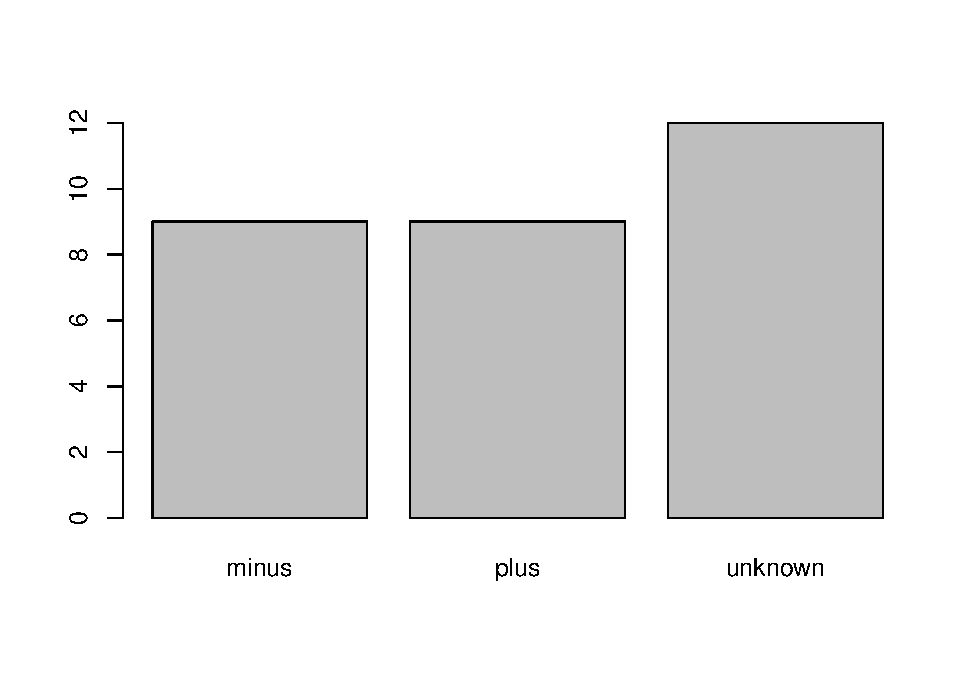
\includegraphics{IntroRWorkshop_files/figure-latex/unnamed-chunk-59-1.pdf}

This isn't a particularly pretty example of a plot. But it can be a useful way to get acquainted with your data.

To reorder the levels of a factor:

\begin{Shaded}
\begin{Highlighting}[]
\NormalTok{cit }\OtherTok{\textless{}{-}} \FunctionTok{factor}\NormalTok{(cit, }\AttributeTok{levels =} \FunctionTok{c}\NormalTok{(}\StringTok{"unknown"}\NormalTok{, }\StringTok{"plus"}\NormalTok{, }\StringTok{"minus"}\NormalTok{))}
\NormalTok{cit}
\end{Highlighting}
\end{Shaded}

\begin{verbatim}
##  [1] unknown unknown unknown unknown unknown unknown unknown unknown unknown
## [10] unknown unknown unknown minus   minus   plus    minus   plus    minus  
## [19] plus    minus   plus    plus    minus   plus    plus    minus   plus   
## [28] minus   plus    minus  
## Levels: unknown plus minus
\end{verbatim}

\begin{Shaded}
\begin{Highlighting}[]
\FunctionTok{plot}\NormalTok{(cit)}
\end{Highlighting}
\end{Shaded}

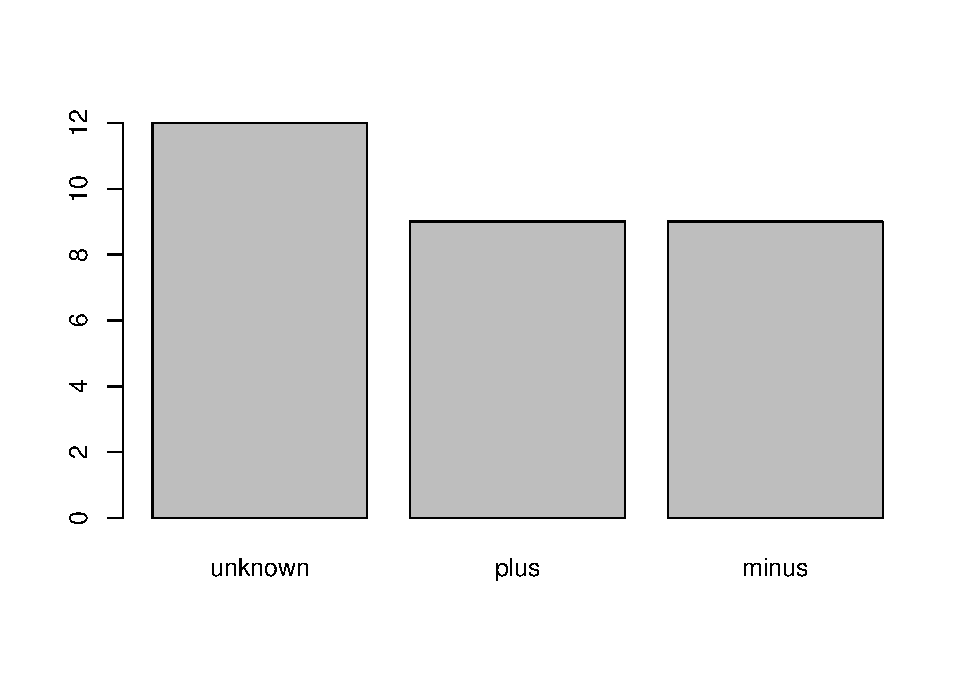
\includegraphics{IntroRWorkshop_files/figure-latex/unnamed-chunk-60-1.pdf}

\hypertarget{subsetting-data-frames}{%
\section{Subsetting data frames}\label{subsetting-data-frames}}

Subsetting data frames is similar to subsetting vectors with one major difference: date frames are two-dimensional. Therefore, to select a specific value we will use the \texttt{{[}{]}} notation again, but we will specify more than one value.

\hypertarget{exercise-6.8.1}{%
\subsubsection*{EXERCISE 6.8.1}\label{exercise-6.8.1}}
\addcontentsline{toc}{subsubsection}{EXERCISE 6.8.1}

Try the following indices on the metadata data frame:

\begin{itemize}
\tightlist
\item
  \texttt{metadata{[}1,1{]}}
\item
  \texttt{metadata{[}4,2{]}}
\item
  \texttt{metadata{[}2,{]}}
\item
  \texttt{metadata{[}1:4,1{]}}
\item
  \texttt{metadata{[},2{]}}
\item
  \texttt{metadata\$run}
\item
  \texttt{metadata{[}metadata\$cit\ ==\ "plus",{]}}
\end{itemize}

What information does the last line tell you?

You can assign a subset of your data frame to a new object. For example, to create a new data frame of only observations from cit- samples:

\begin{Shaded}
\begin{Highlighting}[]
\NormalTok{cit\_minus }\OtherTok{\textless{}{-}}\NormalTok{ metadata[metadata}\SpecialCharTok{$}\NormalTok{cit }\SpecialCharTok{==} \StringTok{"plus"}\NormalTok{,]}
\NormalTok{cit\_minus}
\end{Highlighting}
\end{Shaded}

\begin{verbatim}
##      sample generation clade strain  cit       run genome_size
## 15   ZDB564      31500  Cit+ REL606 plus SRR098289        4.74
## 17   ZDB172      32000  Cit+ REL606 plus SRR098042        4.77
## 19   ZDB143      32500  Cit+ REL606 plus SRR098040        4.79
## 21   CZB152      33000  Cit+ REL606 plus SRR097977        4.80
## 22   CZB154      33000  Cit+ REL606 plus SRR098026        4.76
## 24    ZDB87      34000    C2 REL606 plus SRR098035        4.75
## 25    ZDB96      36000  Cit+ REL606 plus SRR098036        4.74
## 27   ZDB107      38000  Cit+ REL606 plus SRR098038        4.79
## 29 REL10979      40000  Cit+ REL606 plus SRR098029        4.78
\end{verbatim}

\hypertarget{other-data-types}{%
\section{Other data types}\label{other-data-types}}

So far, we have looked at three data types: vectors, data frames, and factors. Here we will briefly cover matrices and lists. These two are not as useful but you may come across them. Later on in the workshop we will discuss tibbles, the tidyverse equivalent of the data frame.

\hypertarget{matrices}{%
\subsection*{Matrices}\label{matrices}}
\addcontentsline{toc}{subsection}{Matrices}

A matrix is a two-dimensional rectangular dataset. It can be created by using a vector input to the matrix function.

\begin{Shaded}
\begin{Highlighting}[]
\NormalTok{m }\OtherTok{\textless{}{-}} \FunctionTok{matrix}\NormalTok{( }\FunctionTok{c}\NormalTok{(}\StringTok{"a"}\NormalTok{,}\StringTok{"a"}\NormalTok{,}\StringTok{"b"}\NormalTok{,}\StringTok{"c"}\NormalTok{,}\StringTok{"b"}\NormalTok{,}\StringTok{"a"}\NormalTok{), }\AttributeTok{nrow =} \DecValTok{2}\NormalTok{, }\AttributeTok{ncol =} \DecValTok{3}\NormalTok{, }\AttributeTok{byrow =} \ConstantTok{TRUE}\NormalTok{)}
\NormalTok{m}
\end{Highlighting}
\end{Shaded}

\begin{verbatim}
##      [,1] [,2] [,3]
## [1,] "a"  "a"  "b" 
## [2,] "c"  "b"  "a"
\end{verbatim}

To output the dimensions of a matrix, use the \texttt{dim()} function.

\begin{Shaded}
\begin{Highlighting}[]
\FunctionTok{dim}\NormalTok{(m) }
\end{Highlighting}
\end{Shaded}

\begin{verbatim}
## [1] 2 3
\end{verbatim}

R will list the number of rows first and the number of columns second. To list only the number of rows or the number of columns, use the \texttt{nrow()} and \texttt{ncol()}. The \texttt{length()} function will output the total number of elements.

\begin{Shaded}
\begin{Highlighting}[]
\FunctionTok{nrow}\NormalTok{(m)}
\end{Highlighting}
\end{Shaded}

\begin{verbatim}
## [1] 2
\end{verbatim}

\begin{Shaded}
\begin{Highlighting}[]
\FunctionTok{ncol}\NormalTok{(m)}
\end{Highlighting}
\end{Shaded}

\begin{verbatim}
## [1] 3
\end{verbatim}

\begin{Shaded}
\begin{Highlighting}[]
\FunctionTok{length}\NormalTok{(m)}
\end{Highlighting}
\end{Shaded}

\begin{verbatim}
## [1] 6
\end{verbatim}

\hypertarget{lists}{%
\subsection*{Lists}\label{lists}}
\addcontentsline{toc}{subsection}{Lists}

A list is an R-object which can contain many different types of elements inside it like vectors, functions, and even another list.

\begin{Shaded}
\begin{Highlighting}[]
\CommentTok{\# Create a list}
\NormalTok{list1 }\OtherTok{\textless{}{-}} \FunctionTok{list}\NormalTok{(}\FunctionTok{c}\NormalTok{(}\DecValTok{2}\NormalTok{,}\DecValTok{5}\NormalTok{,}\DecValTok{3}\NormalTok{),}\FloatTok{21.3}\NormalTok{, BMI)}
\NormalTok{list1}
\end{Highlighting}
\end{Shaded}

\begin{verbatim}
## [[1]]
## [1] 2 5 3
## 
## [[2]]
## [1] 21.3
## 
## [[3]]
##   gender height weight age
## 1   male  152.0     81  42
## 2   male  171.5     93  36
## 3 female  165.0     78  26
\end{verbatim}

\hypertarget{manipulating-data-in-the-tidyverse}{%
\chapter{Manipulating Data in the tidyverse}\label{manipulating-data-in-the-tidyverse}}

\hypertarget{what-is-the-tidyverse}{%
\section{What is the Tidyverse}\label{what-is-the-tidyverse}}

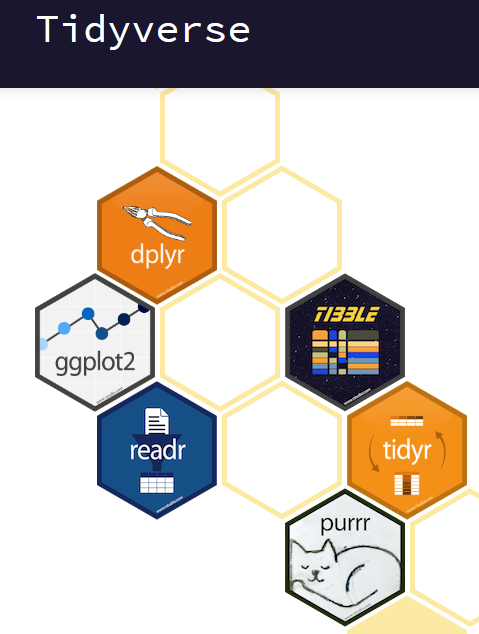
\includegraphics{./figures/tidyverse.png}
The tidyverse is an opinionated collection of R packages designed for data science. All packages share an underlying design philosophy, grammar, and data structures. These packages include:

\begin{itemize}
\tightlist
\item
  \texttt{dplyr} for data manipulation
\item
  \texttt{tibble} for data organizing
\item
  \texttt{ggplot2} for data visualization
\item
  \texttt{tidyr} for \emph{tidy}-ing your data
\item
  \texttt{readr} for reading data into R
\end{itemize}

When we installed the \texttt{tidyverse} package, we installed all of the above packages. This means that all of the specialized functions of these packages are available to use.

\hypertarget{tibbles}{%
\section{Tibbles}\label{tibbles}}

Tibbles are a modern take on data frames. They keep the features that have stood the test of time and drop the features that used to be convenient but are now frustrating (ie. converting character vectors to factors).

\hypertarget{create-a-tibble}{%
\subsection*{Create a tibble}\label{create-a-tibble}}
\addcontentsline{toc}{subsection}{Create a tibble}

You can create a tibble using the \texttt{tibble()} function:

\begin{Shaded}
\begin{Highlighting}[]
\CommentTok{\# Create}
\NormalTok{friends\_data }\OtherTok{\textless{}{-}} \FunctionTok{tibble}\NormalTok{(}
  \AttributeTok{name =} \FunctionTok{c}\NormalTok{(}\StringTok{"Nicolas"}\NormalTok{, }\StringTok{"Thierry"}\NormalTok{, }\StringTok{"Bernard"}\NormalTok{, }\StringTok{"Jerome"}\NormalTok{),}
  \AttributeTok{age =} \FunctionTok{c}\NormalTok{(}\DecValTok{27}\NormalTok{, }\DecValTok{25}\NormalTok{, }\DecValTok{29}\NormalTok{, }\DecValTok{26}\NormalTok{),}
  \AttributeTok{height =} \FunctionTok{c}\NormalTok{(}\DecValTok{180}\NormalTok{, }\DecValTok{170}\NormalTok{, }\DecValTok{185}\NormalTok{, }\DecValTok{169}\NormalTok{),}
  \AttributeTok{married =} \FunctionTok{c}\NormalTok{(}\ConstantTok{TRUE}\NormalTok{, }\ConstantTok{FALSE}\NormalTok{, }\ConstantTok{TRUE}\NormalTok{, }\ConstantTok{TRUE}\NormalTok{)}
\NormalTok{)}
\CommentTok{\# Print}
\NormalTok{friends\_data}
\end{Highlighting}
\end{Shaded}

\begin{verbatim}
## # A tibble: 4 x 4
##   name      age height married
##   <chr>   <dbl>  <dbl> <lgl>  
## 1 Nicolas    27    180 TRUE   
## 2 Thierry    25    170 FALSE  
## 3 Bernard    29    185 TRUE   
## 4 Jerome     26    169 TRUE
\end{verbatim}

\hypertarget{reading-in-tibbles}{%
\subsection*{Reading in tibbles}\label{reading-in-tibbles}}
\addcontentsline{toc}{subsection}{Reading in tibbles}

Tibbles can be read into R using the \texttt{read\_csv()} function. Note that the \texttt{read\_csv()} function is different than the \texttt{read.csv()} function. The major difference is that \texttt{read\_csv()} will store the data as a tibble and \texttt{read.csv()} will store the data as a data frame.

\hypertarget{exercise-7.3.1}{%
\subsubsection*{EXERCISE 7.3.1}\label{exercise-7.3.1}}
\addcontentsline{toc}{subsubsection}{EXERCISE 7.3.1}

Use the \texttt{read\_csv()} function to read in the \texttt{Ecoli\_metadata.csv} file. Assign the data to an object called \texttt{metadata2} to avoid writing over the object \texttt{metadata}.

How is it different that the \texttt{metadata}object?

\hypertarget{data-frames-versus-tibbles}{%
\subsection*{Data frames versus tibbles}\label{data-frames-versus-tibbles}}
\addcontentsline{toc}{subsection}{Data frames versus tibbles}

For some applications, you will need to use data frames and for others tibbles. You will find that some older functions don't work on tibbles. They can be easily converted using the functions \texttt{as.data.frame()} or \texttt{as\_tibble()}:

\begin{Shaded}
\begin{Highlighting}[]
\FunctionTok{head}\NormalTok{(metadata)}
\end{Highlighting}
\end{Shaded}

\begin{verbatim}
##     sample generation   clade strain     cit       run genome_size
## 1   REL606          0     N/A REL606 unknown                  4.62
## 2 REL1166A       2000 unknown REL606 unknown SRR098028        4.63
## 3   ZDB409       5000 unknown REL606 unknown SRR098281        4.60
## 4   ZDB429      10000      UC REL606 unknown SRR098282        4.59
## 5   ZDB446      15000      UC REL606 unknown SRR098283        4.66
## 6   ZDB458      20000 (C1,C2) REL606 unknown SRR098284        4.63
\end{verbatim}

\begin{Shaded}
\begin{Highlighting}[]
\NormalTok{metadata\_tib }\OtherTok{\textless{}{-}} \FunctionTok{as\_tibble}\NormalTok{(metadata)}
\NormalTok{metadata\_tib}
\end{Highlighting}
\end{Shaded}

\begin{verbatim}
## # A tibble: 30 x 7
##    sample   generation clade   strain cit     run         genome_size
##    <chr>         <int> <chr>   <chr>  <chr>   <chr>             <dbl>
##  1 REL606            0 N/A     REL606 unknown ""                 4.62
##  2 REL1166A       2000 unknown REL606 unknown "SRR098028"        4.63
##  3 ZDB409         5000 unknown REL606 unknown "SRR098281"        4.6 
##  4 ZDB429        10000 UC      REL606 unknown "SRR098282"        4.59
##  5 ZDB446        15000 UC      REL606 unknown "SRR098283"        4.66
##  6 ZDB458        20000 (C1,C2) REL606 unknown "SRR098284"        4.63
##  7 ZDB464*       20000 (C1,C2) REL606 unknown "SRR098285"        4.62
##  8 ZDB467        20000 (C1,C2) REL606 unknown "SRR098286"        4.61
##  9 ZDB477        25000 C1      REL606 unknown "SRR098287"        4.65
## 10 ZDB483        25000 C3      REL606 unknown "SRR098288"        4.59
## # ... with 20 more rows
\end{verbatim}

\begin{Shaded}
\begin{Highlighting}[]
\NormalTok{metadata\_df }\OtherTok{\textless{}{-}} \FunctionTok{as.data.frame}\NormalTok{(metadata\_tib)}
\FunctionTok{head}\NormalTok{(metadata\_df)}
\end{Highlighting}
\end{Shaded}

\begin{verbatim}
##     sample generation   clade strain     cit       run genome_size
## 1   REL606          0     N/A REL606 unknown                  4.62
## 2 REL1166A       2000 unknown REL606 unknown SRR098028        4.63
## 3   ZDB409       5000 unknown REL606 unknown SRR098281        4.60
## 4   ZDB429      10000      UC REL606 unknown SRR098282        4.59
## 5   ZDB446      15000      UC REL606 unknown SRR098283        4.66
## 6   ZDB458      20000 (C1,C2) REL606 unknown SRR098284        4.63
\end{verbatim}

\hypertarget{brain-teaser}{%
\subsubsection*{Brain Teaser}\label{brain-teaser}}
\addcontentsline{toc}{subsubsection}{Brain Teaser}

Can a tibble contain different data types in each column?

As you will see in the following sections, many of the useful data frame functions are the same for tibbles.

\hypertarget{exploring-tibbles}{%
\section{Exploring tibbles}\label{exploring-tibbles}}

We can explore the contents of a tibble in several ways. By typing the name of the tibble in the console, we can view the first ten rows of a tibble as above, which tells us lots of information about the column types and the number of rows. We can also use the \texttt{glimpse()} function:

\begin{Shaded}
\begin{Highlighting}[]
\FunctionTok{glimpse}\NormalTok{(metadata\_tib)}
\end{Highlighting}
\end{Shaded}

\begin{verbatim}
## Rows: 30
## Columns: 7
## $ sample      <chr> "REL606", "REL1166A", "ZDB409", "ZDB429", "ZDB446", "ZDB45~
## $ generation  <int> 0, 2000, 5000, 10000, 15000, 20000, 20000, 20000, 25000, 2~
## $ clade       <chr> "N/A", "unknown", "unknown", "UC", "UC", "(C1,C2)", "(C1,C~
## $ strain      <chr> "REL606", "REL606", "REL606", "REL606", "REL606", "REL606"~
## $ cit         <chr> "unknown", "unknown", "unknown", "unknown", "unknown", "un~
## $ run         <chr> "", "SRR098028", "SRR098281", "SRR098282", "SRR098283", "S~
## $ genome_size <dbl> 4.62, 4.63, 4.60, 4.59, 4.66, 4.63, 4.62, 4.61, 4.65, 4.59~
\end{verbatim}

As with data frames, we can return a vector containing the values of a variable (column) using the \$ sign:

\begin{Shaded}
\begin{Highlighting}[]
\NormalTok{metadata\_tib}\SpecialCharTok{$}\NormalTok{generation}
\end{Highlighting}
\end{Shaded}

\begin{verbatim}
##  [1]     0  2000  5000 10000 15000 20000 20000 20000 25000 25000 30000 30000
## [13] 31500 31500 31500 32000 32000 32500 32500 33000 33000 33000 34000 34000
## [25] 36000 36000 38000 38000 40000 40000
\end{verbatim}

Again, similar to data frames, we can use the subsetting operator {[}{]} directly on tibbles. A tibble is two-dimensional, so we must pass two arguments to the {[}{]} operator; the first indicates the row(s) we require and the second indicates the column(s). To return the value in row 10, column 1:

\begin{Shaded}
\begin{Highlighting}[]
\NormalTok{metadata\_tib[}\DecValTok{10}\NormalTok{,}\DecValTok{1}\NormalTok{]}
\end{Highlighting}
\end{Shaded}

\begin{verbatim}
## # A tibble: 1 x 1
##   sample
##   <chr> 
## 1 ZDB483
\end{verbatim}

Similarly, to return the values in rows 25 to 30, and columns 1 to 3:

\begin{verbatim}
metadata_tib[25:30, 1:3]
\end{verbatim}

If we leave an index blank, this acts as a wildcard and matches all of the rows or columns:

\begin{Shaded}
\begin{Highlighting}[]
\NormalTok{metadata\_tib[}\DecValTok{22}\NormalTok{,]}
\end{Highlighting}
\end{Shaded}

\begin{verbatim}
## # A tibble: 1 x 7
##   sample generation clade strain cit   run       genome_size
##   <chr>       <int> <chr> <chr>  <chr> <chr>           <dbl>
## 1 CZB154      33000 Cit+  REL606 plus  SRR098026        4.76
\end{verbatim}

\begin{Shaded}
\begin{Highlighting}[]
\NormalTok{metadata\_tib[,}\DecValTok{1}\SpecialCharTok{:}\DecValTok{3}\NormalTok{]}
\end{Highlighting}
\end{Shaded}

\begin{verbatim}
## # A tibble: 30 x 3
##    sample   generation clade  
##    <chr>         <int> <chr>  
##  1 REL606            0 N/A    
##  2 REL1166A       2000 unknown
##  3 ZDB409         5000 unknown
##  4 ZDB429        10000 UC     
##  5 ZDB446        15000 UC     
##  6 ZDB458        20000 (C1,C2)
##  7 ZDB464*       20000 (C1,C2)
##  8 ZDB467        20000 (C1,C2)
##  9 ZDB477        25000 C1     
## 10 ZDB483        25000 C3     
## # ... with 20 more rows
\end{verbatim}

You can also refer to columns by name with quotation marks:

\begin{Shaded}
\begin{Highlighting}[]
\NormalTok{metadata\_tib[,}\StringTok{"sample"}\NormalTok{]}
\end{Highlighting}
\end{Shaded}

\begin{verbatim}
## # A tibble: 30 x 1
##    sample  
##    <chr>   
##  1 REL606  
##  2 REL1166A
##  3 ZDB409  
##  4 ZDB429  
##  5 ZDB446  
##  6 ZDB458  
##  7 ZDB464* 
##  8 ZDB467  
##  9 ZDB477  
## 10 ZDB483  
## # ... with 20 more rows
\end{verbatim}

Note that subsetting a tibble using the {[}{]} method returns another tibble. In contrast, using the \$ sign to extract a variable returns a vector:

\begin{Shaded}
\begin{Highlighting}[]
\NormalTok{metadata\_tib}\SpecialCharTok{$}\NormalTok{sample}
\end{Highlighting}
\end{Shaded}

\begin{verbatim}
##  [1] "REL606"   "REL1166A" "ZDB409"   "ZDB429"   "ZDB446"   "ZDB458"  
##  [7] "ZDB464*"  "ZDB467"   "ZDB477"   "ZDB483"   "ZDB16"    "ZDB357"  
## [13] "ZDB199*"  "ZDB200"   "ZDB564"   "ZDB30*"   "ZDB172"   "ZDB158"  
## [19] "ZDB143"   "CZB199"   "CZB152"   "CZB154"   "ZDB83"    "ZDB87"   
## [25] "ZDB96"    "ZDB99"    "ZDB107"   "ZDB111"   "REL10979" "REL10988"
\end{verbatim}

For more information on tibbles see the \href{https://cran.r-project.org/web/packages/tibble/vignettes/tibble.html}{tibbles vignette}.

\hypertarget{tidy-data}{%
\section{Tidy data}\label{tidy-data}}

Tidy data is data that's easy to work with: it's easy to manage (with dplyr), visualize (with ggplot2) and model (with R's hundreds of modeling packages). Most importantly, tidy data is data where \textbf{each column is a variable} and \textbf{each row is an observation}.

Arranging your data in this way makes it easier to work with because you have a consistent way of referring to variables (as column names) and observations (as row indices). When use tidy data and tidy tools, you spend less time worrying about how to feed the output from one function into the input of another, and more time answering your questions about the data.

To tidy messy data, you first identify the variables in your dataset, then use the tools provided by \texttt{tidyr} to move them into columns. \texttt{tidyr} provides three main functions for tidying your messy data:

\begin{itemize}
\tightlist
\item
  \texttt{gather()}
\item
  \texttt{separate()}
\item
  \texttt{spread()}
\end{itemize}

\hypertarget{gather}{%
\subsection*{\texorpdfstring{\texttt{gather()}}{gather()}}\label{gather}}
\addcontentsline{toc}{subsection}{\texttt{gather()}}


\includegraphics{./figures/tidyr-gather.png}

The \texttt{gather()} function takes multiple columns, and gathers them into key-value pairs: it makes ``wide'' data longer. Here's an example. In this experiment we've given three people two different drugs and recorded their heart rate:

\begin{Shaded}
\begin{Highlighting}[]
\NormalTok{messy }\OtherTok{\textless{}{-}} \FunctionTok{data.frame}\NormalTok{(}
  \AttributeTok{name =} \FunctionTok{c}\NormalTok{(}\StringTok{"Wilbur"}\NormalTok{, }\StringTok{"Petunia"}\NormalTok{, }\StringTok{"Gregory"}\NormalTok{),}
  \AttributeTok{drugA =} \FunctionTok{c}\NormalTok{(}\DecValTok{67}\NormalTok{, }\DecValTok{80}\NormalTok{, }\DecValTok{64}\NormalTok{),}
  \AttributeTok{drugB =} \FunctionTok{c}\NormalTok{(}\DecValTok{56}\NormalTok{, }\DecValTok{90}\NormalTok{, }\DecValTok{50}\NormalTok{)}
\NormalTok{)}
\NormalTok{messy}
\end{Highlighting}
\end{Shaded}

\begin{verbatim}
##      name drugA drugB
## 1  Wilbur    67    56
## 2 Petunia    80    90
## 3 Gregory    64    50
\end{verbatim}

We have three variables (name, drug and heartrate), but only name is currently in a column. We use \texttt{gather()} to gather the a and b columns into key-value pairs of drug and heartrate:

\begin{Shaded}
\begin{Highlighting}[]
  \FunctionTok{gather}\NormalTok{(messy,drug, heartrate, drugA}\SpecialCharTok{:}\NormalTok{drugB)}
\end{Highlighting}
\end{Shaded}

\begin{verbatim}
##      name  drug heartrate
## 1  Wilbur drugA        67
## 2 Petunia drugA        80
## 3 Gregory drugA        64
## 4  Wilbur drugB        56
## 5 Petunia drugB        90
## 6 Gregory drugB        50
\end{verbatim}

Now each column is a variable and each row is an observation - tidy! Note: more about the ``pipe'' operator later.

\hypertarget{exercise-7.4.1}{%
\subsubsection*{EXERCISE 7.4.1}\label{exercise-7.4.1}}
\addcontentsline{toc}{subsubsection}{EXERCISE 7.4.1}

\begin{enumerate}
\def\labelenumi{\arabic{enumi}.}
\item
  In this example, what is the key and what is the value?
  \texttt{gather(messy,drug,\ heartrate,\ drugA:drugB)}
\item
  What does drugA:drugB mean?
\item
  What is the difference between long and wide data?
\end{enumerate}

\hypertarget{separate}{%
\subsection*{\texorpdfstring{\texttt{separate()}}{separate()}}\label{separate}}
\addcontentsline{toc}{subsection}{\texttt{separate()}}


\includegraphics{./figures/tidyr-separate.png}

Sometimes two variables are clumped together in one column. separate() allows you to tease them apart. We have some measurements of how much time people spend on their phones, measured at two locations (work and home), at two times. Each person has been randomly assigned to either treatment or control.

\begin{Shaded}
\begin{Highlighting}[]
\NormalTok{messy}
\end{Highlighting}
\end{Shaded}

\begin{verbatim}
##   id       trt    work.T1   home.T1   work.T2    home.T2
## 1  1 treatment 0.08513597 0.6158293 0.1135090 0.05190332
## 2  2   control 0.22543662 0.4296715 0.5959253 0.26417767
## 3  3   control 0.27453052 0.6516557 0.3580500 0.39879073
## 4  4 treatment 0.27230507 0.5677378 0.4288094 0.83613414
\end{verbatim}

To tidy this data, we first use gather() to turn columns work.T1, home.T1, work.T2 and home.T2 into a key-value pair of key and time:

\begin{Shaded}
\begin{Highlighting}[]
\NormalTok{tidier }\OtherTok{\textless{}{-}}  \FunctionTok{gather}\NormalTok{(messy,key, time, }\SpecialCharTok{{-}}\NormalTok{id, }\SpecialCharTok{{-}}\NormalTok{trt)}
\NormalTok{tidier}
\end{Highlighting}
\end{Shaded}

\begin{verbatim}
##    id       trt     key       time
## 1   1 treatment work.T1 0.08513597
## 2   2   control work.T1 0.22543662
## 3   3   control work.T1 0.27453052
## 4   4 treatment work.T1 0.27230507
## 5   1 treatment home.T1 0.61582931
## 6   2   control home.T1 0.42967153
## 7   3   control home.T1 0.65165567
## 8   4 treatment home.T1 0.56773775
## 9   1 treatment work.T2 0.11350898
## 10  2   control work.T2 0.59592531
## 11  3   control work.T2 0.35804998
## 12  4 treatment work.T2 0.42880942
## 13  1 treatment home.T2 0.05190332
## 14  2   control home.T2 0.26417767
## 15  3   control home.T2 0.39879073
## 16  4 treatment home.T2 0.83613414
\end{verbatim}

Next we use separate() to split the key into location and time, using a regular expression to describe the character that separates them:

\begin{Shaded}
\begin{Highlighting}[]
\NormalTok{tidy }\OtherTok{\textless{}{-}} \FunctionTok{separate}\NormalTok{(tidier,key, }\AttributeTok{into =} \FunctionTok{c}\NormalTok{(}\StringTok{"location"}\NormalTok{, }\StringTok{"timepoint"}\NormalTok{), }\AttributeTok{sep =} \StringTok{"}\SpecialCharTok{\textbackslash{}\textbackslash{}}\StringTok{."}\NormalTok{)}
\NormalTok{tidy}
\end{Highlighting}
\end{Shaded}

\begin{verbatim}
##    id       trt location timepoint       time
## 1   1 treatment     work        T1 0.08513597
## 2   2   control     work        T1 0.22543662
## 3   3   control     work        T1 0.27453052
## 4   4 treatment     work        T1 0.27230507
## 5   1 treatment     home        T1 0.61582931
## 6   2   control     home        T1 0.42967153
## 7   3   control     home        T1 0.65165567
## 8   4 treatment     home        T1 0.56773775
## 9   1 treatment     work        T2 0.11350898
## 10  2   control     work        T2 0.59592531
## 11  3   control     work        T2 0.35804998
## 12  4 treatment     work        T2 0.42880942
## 13  1 treatment     home        T2 0.05190332
## 14  2   control     home        T2 0.26417767
## 15  3   control     home        T2 0.39879073
## 16  4 treatment     home        T2 0.83613414
\end{verbatim}

You can also use integer position to split at.

\hypertarget{brain-teaser-1}{%
\subsubsection*{Brain Teaser}\label{brain-teaser-1}}
\addcontentsline{toc}{subsubsection}{Brain Teaser}

Why do we have ``\textbackslash{}'' before ``.'' in sep=''\textbackslash.''

\hypertarget{spread}{%
\subsection*{\texorpdfstring{\texttt{spread()}}{spread()}}\label{spread}}
\addcontentsline{toc}{subsection}{\texttt{spread()}}


\includegraphics{./figures/tidyr-spread.png}

The function \texttt{spread()} does the reverse of \texttt{gather()}. It takes two columns and spreads them into multiple columns. It produces ``wide'' data from ``long'' data. Typically you will want your data in a wide form so you likely won't use this much. See the documentation for more information.

\hypertarget{what-is-dplyr}{%
\section{What is dplyr?}\label{what-is-dplyr}}

The package \texttt{dplyr} is a package that tries to provide easy tools for the most common data manipulation tasks. It is built to work directly with tibbles. The thinking behind it was largely inspired by the package \texttt{plyr} which has been in use for some time but suffered from being slow in some cases. \texttt{dplyr} addresses this by porting much of the computation to C++. An additional feature is the ability to work with data stored directly in an external database. The benefits of doing this are that the data can be managed natively in a relational database, queries can be conducted on that database, and only the results of the query returned.

This addresses a common problem with R in that all operations are conducted in memory and thus the amount of data you can work with is limited by available memory. The database connections essentially remove that limitation in that you can have a database of many 100s GB, conduct queries on it directly and pull back just what you need for analysis in R.

\hypertarget{selecting-columns-and-filtering-rows}{%
\section{Selecting columns and filtering rows}\label{selecting-columns-and-filtering-rows}}

We're going to learn some of the most common \texttt{dplyr} functions: \texttt{select()}, \texttt{filter()}, \texttt{mutate()}, \texttt{group\_by()}, and \texttt{summarize()}. To select columns of a data frame, use \texttt{select()}. The first argument to this function is the data frame (tibble), and the subsequent arguments are the columns to keep.

\begin{Shaded}
\begin{Highlighting}[]
\FunctionTok{select}\NormalTok{(metadata, sample, clade, cit, genome\_size)}
\end{Highlighting}
\end{Shaded}

\begin{verbatim}
##      sample   clade     cit genome_size
## 1    REL606     N/A unknown        4.62
## 2  REL1166A unknown unknown        4.63
## 3    ZDB409 unknown unknown        4.60
## 4    ZDB429      UC unknown        4.59
## 5    ZDB446      UC unknown        4.66
## 6    ZDB458 (C1,C2) unknown        4.63
## 7   ZDB464* (C1,C2) unknown        4.62
## 8    ZDB467 (C1,C2) unknown        4.61
## 9    ZDB477      C1 unknown        4.65
## 10   ZDB483      C3 unknown        4.59
## 11    ZDB16      C1 unknown        4.61
## 12   ZDB357      C2 unknown        4.62
## 13  ZDB199*      C1   minus        4.62
## 14   ZDB200      C2   minus        4.63
## 15   ZDB564    Cit+    plus        4.74
## 16   ZDB30*      C3   minus        4.61
## 17   ZDB172    Cit+    plus        4.77
## 18   ZDB158      C2   minus        4.63
## 19   ZDB143    Cit+    plus        4.79
## 20   CZB199      C1   minus        4.59
## 21   CZB152    Cit+    plus        4.80
## 22   CZB154    Cit+    plus        4.76
## 23    ZDB83    Cit+   minus        4.60
## 24    ZDB87      C2    plus        4.75
## 25    ZDB96    Cit+    plus        4.74
## 26    ZDB99      C1   minus        4.61
## 27   ZDB107    Cit+    plus        4.79
## 28   ZDB111      C2   minus        4.62
## 29 REL10979    Cit+    plus        4.78
## 30 REL10988      C2   minus        4.62
\end{verbatim}

\hypertarget{exercise-7.6.1}{%
\subsubsection*{EXERCISE 7.6.1}\label{exercise-7.6.1}}
\addcontentsline{toc}{subsubsection}{EXERCISE 7.6.1}

Would the two calls to the select function below return the same tibble or not?

\texttt{select(metadata,\ sample,\ clade,\ cit,\ genome\_size)}

\texttt{select(metadata,\ -generation,-strain,-run)}

To choose rows, use filter():

\begin{Shaded}
\begin{Highlighting}[]
\FunctionTok{filter}\NormalTok{(metadata, cit }\SpecialCharTok{==} \StringTok{"plus"}\NormalTok{)}
\end{Highlighting}
\end{Shaded}

\begin{verbatim}
##     sample generation clade strain  cit       run genome_size
## 1   ZDB564      31500  Cit+ REL606 plus SRR098289        4.74
## 2   ZDB172      32000  Cit+ REL606 plus SRR098042        4.77
## 3   ZDB143      32500  Cit+ REL606 plus SRR098040        4.79
## 4   CZB152      33000  Cit+ REL606 plus SRR097977        4.80
## 5   CZB154      33000  Cit+ REL606 plus SRR098026        4.76
## 6    ZDB87      34000    C2 REL606 plus SRR098035        4.75
## 7    ZDB96      36000  Cit+ REL606 plus SRR098036        4.74
## 8   ZDB107      38000  Cit+ REL606 plus SRR098038        4.79
## 9 REL10979      40000  Cit+ REL606 plus SRR098029        4.78
\end{verbatim}

\hypertarget{exercise-7.6.2}{%
\subsubsection*{EXERCISE 7.6.2}\label{exercise-7.6.2}}
\addcontentsline{toc}{subsubsection}{EXERCISE 7.6.2}

\begin{enumerate}
\def\labelenumi{\arabic{enumi}.}
\tightlist
\item
  Keep only the rows that are not cit = plus.
\item
  Keep only the rows for samples taken in the first 30000 generations.
\end{enumerate}

\hypertarget{pipes}{%
\section{Pipes}\label{pipes}}

But what if you wanted to \texttt{select} and \texttt{filter}? There are three ways to do this: use intermediate steps, nested functions, or pipes. With the intermediate steps, you essentially create a temporary data frame and use that as input to the next function. This can clutter up your workspace with lots of objects. You can also nest functions (i.e.~one function inside of another). This is handy, but can be difficult to read if too many functions are nested as the process from inside out. The last option, pipes, are a fairly recent addition to R. Pipes let you take the output of one function and send it directly to the next, which is useful when you need to many things to the same data set. Pipes in R look like \texttt{\%\textgreater{}\%} and are made available via the \texttt{magrittr} package installed as part of tidyverse. If you're familiar with the Unix shell, you may already have used pipes to pass the output from one command to the next. The concept is the same, except the shell uses the \texttt{\textbar{}} character rather than R's pipe operator \texttt{\%\textgreater{}\%}.

The pipe operator can be tedious to type. In Rstudio pressing \texttt{Ctrl\ +\ Shift\ +\ M} under Windows / Linux will insert the pipe operator. On the mac, use \texttt{⌘\ +\ Shift\ +\ M}.

\begin{Shaded}
\begin{Highlighting}[]
\NormalTok{metadata }\SpecialCharTok{\%\textgreater{}\%}
  \FunctionTok{filter}\NormalTok{(cit }\SpecialCharTok{==} \StringTok{"plus"}\NormalTok{) }\SpecialCharTok{\%\textgreater{}\%}
  \FunctionTok{select}\NormalTok{(sample, generation, clade, cit)}
\end{Highlighting}
\end{Shaded}

\begin{verbatim}
##     sample generation clade  cit
## 1   ZDB564      31500  Cit+ plus
## 2   ZDB172      32000  Cit+ plus
## 3   ZDB143      32500  Cit+ plus
## 4   CZB152      33000  Cit+ plus
## 5   CZB154      33000  Cit+ plus
## 6    ZDB87      34000    C2 plus
## 7    ZDB96      36000  Cit+ plus
## 8   ZDB107      38000  Cit+ plus
## 9 REL10979      40000  Cit+ plus
\end{verbatim}

In the above we use the pipe to send the data set first through \texttt{filter}, to keep rows where cit was equal to `plus', and then through \texttt{select} to keep the sample and generation and clade columns. When the data frame is being passed to the \texttt{filter()} and \texttt{select()} functions through a pipe, we don't need to include it as an argument to these functions anymore.

\hypertarget{exercise-7.7.1}{%
\subsubsection*{EXERCISE 7.7.1}\label{exercise-7.7.1}}
\addcontentsline{toc}{subsubsection}{EXERCISE 7.7.1}

Does the order of \texttt{filter()} and \texttt{select()} above matter? Why or why not?

Answer to yourself or to a neighbour and then confirm your answer by trying it both ways.

Note that the above is the same as the nested version:

\begin{Shaded}
\begin{Highlighting}[]
\FunctionTok{select}\NormalTok{(}\FunctionTok{filter}\NormalTok{(metadata, cit }\SpecialCharTok{==} \StringTok{"plus"}\NormalTok{), sample, generation, clade)}
\end{Highlighting}
\end{Shaded}

\begin{verbatim}
##     sample generation clade
## 1   ZDB564      31500  Cit+
## 2   ZDB172      32000  Cit+
## 3   ZDB143      32500  Cit+
## 4   CZB152      33000  Cit+
## 5   CZB154      33000  Cit+
## 6    ZDB87      34000    C2
## 7    ZDB96      36000  Cit+
## 8   ZDB107      38000  Cit+
## 9 REL10979      40000  Cit+
\end{verbatim}

If we wanted to create a new object with this smaller version of the data we could do so by assigning it a new name:

\begin{Shaded}
\begin{Highlighting}[]
\NormalTok{Ecoli\_citplus }\OtherTok{\textless{}{-}}\NormalTok{ metadata }\SpecialCharTok{\%\textgreater{}\%}
  \FunctionTok{filter}\NormalTok{(cit }\SpecialCharTok{==} \StringTok{"plus"}\NormalTok{) }\SpecialCharTok{\%\textgreater{}\%}
  \FunctionTok{select}\NormalTok{(sample, generation, clade)}

\NormalTok{Ecoli\_citplus}
\end{Highlighting}
\end{Shaded}

\begin{verbatim}
##     sample generation clade
## 1   ZDB564      31500  Cit+
## 2   ZDB172      32000  Cit+
## 3   ZDB143      32500  Cit+
## 4   CZB152      33000  Cit+
## 5   CZB154      33000  Cit+
## 6    ZDB87      34000    C2
## 7    ZDB96      36000  Cit+
## 8   ZDB107      38000  Cit+
## 9 REL10979      40000  Cit+
\end{verbatim}

We can think of the \texttt{filter()} and \texttt{select()} functions as verbs in the sentence; they do things to the data flowing through the pipeline.

\hypertarget{exercise-7.7.2}{%
\subsubsection*{EXERCISE 7.7.2}\label{exercise-7.7.2}}
\addcontentsline{toc}{subsubsection}{EXERCISE 7.7.2}

Using pipes, subset \texttt{metadata} to include rows where the clade is `Cit+' and keep only the columns \texttt{sample}, \texttt{cit}, and \texttt{genome\_size}.
How many rows are in that tibble?

\hypertarget{mutate}{%
\section{Mutate}\label{mutate}}

Frequently you'll want to create new columns based on the values in existing columns, for example to do unit conversions or find the ratio of values in two columns. For this we'll use \texttt{mutate()}.

To create a new column of genome size in bp:

\begin{Shaded}
\begin{Highlighting}[]
\NormalTok{metadata }\SpecialCharTok{\%\textgreater{}\%}
  \FunctionTok{mutate}\NormalTok{(}\AttributeTok{genome\_bp =}\NormalTok{ genome\_size }\SpecialCharTok{*}\FloatTok{1e6}\NormalTok{)}
\end{Highlighting}
\end{Shaded}

\begin{verbatim}
##      sample generation   clade strain     cit       run genome_size genome_bp
## 1    REL606          0     N/A REL606 unknown                  4.62   4620000
## 2  REL1166A       2000 unknown REL606 unknown SRR098028        4.63   4630000
## 3    ZDB409       5000 unknown REL606 unknown SRR098281        4.60   4600000
## 4    ZDB429      10000      UC REL606 unknown SRR098282        4.59   4590000
## 5    ZDB446      15000      UC REL606 unknown SRR098283        4.66   4660000
## 6    ZDB458      20000 (C1,C2) REL606 unknown SRR098284        4.63   4630000
## 7   ZDB464*      20000 (C1,C2) REL606 unknown SRR098285        4.62   4620000
## 8    ZDB467      20000 (C1,C2) REL606 unknown SRR098286        4.61   4610000
## 9    ZDB477      25000      C1 REL606 unknown SRR098287        4.65   4650000
## 10   ZDB483      25000      C3 REL606 unknown SRR098288        4.59   4590000
## 11    ZDB16      30000      C1 REL606 unknown SRR098031        4.61   4610000
## 12   ZDB357      30000      C2 REL606 unknown SRR098280        4.62   4620000
## 13  ZDB199*      31500      C1 REL606   minus SRR098044        4.62   4620000
## 14   ZDB200      31500      C2 REL606   minus SRR098279        4.63   4630000
## 15   ZDB564      31500    Cit+ REL606    plus SRR098289        4.74   4740000
## 16   ZDB30*      32000      C3 REL606   minus SRR098032        4.61   4610000
## 17   ZDB172      32000    Cit+ REL606    plus SRR098042        4.77   4770000
## 18   ZDB158      32500      C2 REL606   minus SRR098041        4.63   4630000
## 19   ZDB143      32500    Cit+ REL606    plus SRR098040        4.79   4790000
## 20   CZB199      33000      C1 REL606   minus SRR098027        4.59   4590000
## 21   CZB152      33000    Cit+ REL606    plus SRR097977        4.80   4800000
## 22   CZB154      33000    Cit+ REL606    plus SRR098026        4.76   4760000
## 23    ZDB83      34000    Cit+ REL606   minus SRR098034        4.60   4600000
## 24    ZDB87      34000      C2 REL606    plus SRR098035        4.75   4750000
## 25    ZDB96      36000    Cit+ REL606    plus SRR098036        4.74   4740000
## 26    ZDB99      36000      C1 REL606   minus SRR098037        4.61   4610000
## 27   ZDB107      38000    Cit+ REL606    plus SRR098038        4.79   4790000
## 28   ZDB111      38000      C2 REL606   minus SRR098039        4.62   4620000
## 29 REL10979      40000    Cit+ REL606    plus SRR098029        4.78   4780000
## 30 REL10988      40000      C2 REL606   minus SRR098030        4.62   4620000
\end{verbatim}

\hypertarget{exercise-7.8.1}{%
\subsubsection*{EXERCISE 7.8.1}\label{exercise-7.8.1}}
\addcontentsline{toc}{subsubsection}{EXERCISE 7.8.1}

\begin{enumerate}
\def\labelenumi{\arabic{enumi}.}
\item
  Use the \texttt{mutate()} function to mutate generation into a fraction from 0 to 1.
\item
  What if you want to change a column instead of create a new column. Can you do that with \texttt{mutate}?
\end{enumerate}

\hypertarget{split-apply-combine-data-analysis-and-the-summarize-function}{%
\section{Split-apply-combine data analysis and the summarize() function}\label{split-apply-combine-data-analysis-and-the-summarize-function}}

Many data analysis tasks can be approached using the ``split-apply-combine'' paradigm: split the data into groups, apply some analysis to each group, and then combine the results. \texttt{dplyr} makes this very easy through the use of the \texttt{group\_by()} function, which splits the data into groups. When the data is grouped in this way \texttt{summarize()} can be used to collapse each group into a single-row summary. \texttt{summarize()} does this by applying an aggregation or summary function to each group. For example, if we wanted to group by citrate-using mutant status and find the number of rows of data for each status, we would do:

\begin{Shaded}
\begin{Highlighting}[]
\NormalTok{metadata }\SpecialCharTok{\%\textgreater{}\%}
  \FunctionTok{group\_by}\NormalTok{(cit) }\SpecialCharTok{\%\textgreater{}\%}
  \FunctionTok{summarize}\NormalTok{(}\FunctionTok{n}\NormalTok{())}
\end{Highlighting}
\end{Shaded}

\begin{verbatim}
## # A tibble: 3 x 2
##   cit     `n()`
##   <chr>   <int>
## 1 minus       9
## 2 plus        9
## 3 unknown    12
\end{verbatim}

Here the summary function used was \texttt{n()} to find the count for each group. We can also apply many other functions to individual columns to get other summary statistics. For example, in the R base package we can use built-in functions like \texttt{mean}, \texttt{median}, \texttt{min}, and \texttt{max}. By default, all R functions operating on vectors that contains missing data will return \texttt{NA}. It's a way to make sure that users know they have missing data, and make a conscious decision on how to deal with it. When dealing with simple statistics like the \texttt{mean}, the easiest way to ignore \texttt{NA} (the missing data) is to use \texttt{na.rm=TRUE} (rm stands for remove).

\hypertarget{exercise-7.9.1}{%
\subsubsection*{EXERCISE 7.9.1}\label{exercise-7.9.1}}
\addcontentsline{toc}{subsubsection}{EXERCISE 7.9.1}

Use the \texttt{group\_by()} and \texttt{summarize()} to view mean \texttt{genome\_size} by mutant status (ie. cit).

You can group by multiple columns too:

\begin{Shaded}
\begin{Highlighting}[]
\NormalTok{metadata }\SpecialCharTok{\%\textgreater{}\%}
  \FunctionTok{group\_by}\NormalTok{(cit, clade) }\SpecialCharTok{\%\textgreater{}\%}
  \FunctionTok{summarize}\NormalTok{(}\AttributeTok{mean\_size =} \FunctionTok{mean}\NormalTok{(genome\_size, }\AttributeTok{na.rm =} \ConstantTok{TRUE}\NormalTok{))}
\end{Highlighting}
\end{Shaded}

\begin{verbatim}
## `summarise()` has grouped output by 'cit'. You can override using the `.groups`
## argument.
\end{verbatim}

\begin{verbatim}
## # A tibble: 13 x 3
## # Groups:   cit [3]
##    cit     clade   mean_size
##    <chr>   <chr>       <dbl>
##  1 minus   C1           4.61
##  2 minus   C2           4.62
##  3 minus   C3           4.61
##  4 minus   Cit+         4.6 
##  5 plus    C2           4.75
##  6 plus    Cit+         4.77
##  7 unknown (C1,C2)      4.62
##  8 unknown C1           4.63
##  9 unknown C2           4.62
## 10 unknown C3           4.59
## 11 unknown N/A          4.62
## 12 unknown UC           4.62
## 13 unknown unknown      4.62
\end{verbatim}

Looks like for one of these clones, the clade is missing. We could then discard those rows using filter():

\begin{Shaded}
\begin{Highlighting}[]
\NormalTok{metadata }\SpecialCharTok{\%\textgreater{}\%}
  \FunctionTok{group\_by}\NormalTok{(cit, clade) }\SpecialCharTok{\%\textgreater{}\%}
  \FunctionTok{summarize}\NormalTok{(}\AttributeTok{mean\_size =} \FunctionTok{mean}\NormalTok{(genome\_size, }\AttributeTok{na.rm =} \ConstantTok{TRUE}\NormalTok{)) }\SpecialCharTok{\%\textgreater{}\%}
  \FunctionTok{filter}\NormalTok{(}\SpecialCharTok{!}\FunctionTok{is.na}\NormalTok{(clade))}
\end{Highlighting}
\end{Shaded}

\begin{verbatim}
## `summarise()` has grouped output by 'cit'. You can override using the `.groups`
## argument.
\end{verbatim}

\begin{verbatim}
## # A tibble: 13 x 3
## # Groups:   cit [3]
##    cit     clade   mean_size
##    <chr>   <chr>       <dbl>
##  1 minus   C1           4.61
##  2 minus   C2           4.62
##  3 minus   C3           4.61
##  4 minus   Cit+         4.6 
##  5 plus    C2           4.75
##  6 plus    Cit+         4.77
##  7 unknown (C1,C2)      4.62
##  8 unknown C1           4.63
##  9 unknown C2           4.62
## 10 unknown C3           4.59
## 11 unknown N/A          4.62
## 12 unknown UC           4.62
## 13 unknown unknown      4.62
\end{verbatim}

You can also summarize multiple variables at the same time:

\begin{Shaded}
\begin{Highlighting}[]
\NormalTok{metadata }\SpecialCharTok{\%\textgreater{}\%}
  \FunctionTok{group\_by}\NormalTok{(cit, clade) }\SpecialCharTok{\%\textgreater{}\%}
  \FunctionTok{summarize}\NormalTok{(}\AttributeTok{mean\_size =} \FunctionTok{mean}\NormalTok{(genome\_size, }\AttributeTok{na.rm =} \ConstantTok{TRUE}\NormalTok{),}
            \AttributeTok{min\_generation =} \FunctionTok{min}\NormalTok{(generation))}
\end{Highlighting}
\end{Shaded}

\begin{verbatim}
## `summarise()` has grouped output by 'cit'. You can override using the `.groups`
## argument.
\end{verbatim}

\begin{verbatim}
## # A tibble: 13 x 4
## # Groups:   cit [3]
##    cit     clade   mean_size min_generation
##    <chr>   <chr>       <dbl>          <int>
##  1 minus   C1           4.61          31500
##  2 minus   C2           4.62          31500
##  3 minus   C3           4.61          32000
##  4 minus   Cit+         4.6           34000
##  5 plus    C2           4.75          34000
##  6 plus    Cit+         4.77          31500
##  7 unknown (C1,C2)      4.62          20000
##  8 unknown C1           4.63          25000
##  9 unknown C2           4.62          30000
## 10 unknown C3           4.59          25000
## 11 unknown N/A          4.62              0
## 12 unknown UC           4.62          10000
## 13 unknown unknown      4.62           2000
\end{verbatim}

For a summary of the tidyr and dplyr functions, see this \href{http://www.rstudio.com/wp-content/uploads/2015/02/data-wrangling-cheatsheet.pdf}{Handy dplyr cheatsheet}.

\hypertarget{exercise-7.9.2}{%
\subsubsection*{EXERCISE 7.9.2}\label{exercise-7.9.2}}
\addcontentsline{toc}{subsubsection}{EXERCISE 7.9.2}

Create a tibble containing each unique clade (removing the samples with unknown clades) and the rank of it's mean genome size. (note that ranking genome size will not sort the table; the row order will be unchanged. You can use the \texttt{arrange()} function to sort the table).

There are several functions for ranking observations, which handle tied values differently. For this exercise it doesn't matter which function you choose. Use the help options to find a ranking function.

\hypertarget{other-great-resources}{%
\section{Other great resources}\label{other-great-resources}}

\begin{itemize}
\tightlist
\item
  \href{https://suzan.rbind.io/categories/tutorial/}{Data Wrangling tutorial} - an excellent four part tutorial covering selecting data, filtering data, summarising and transforming your data.
\item
  \href{http://r4ds.had.co.nz/}{R for Data Science}
\item
  \href{https://www.rstudio.com/resources/webinars/data-wrangling-with-r-and-rstudio/}{Data wrangling with R and RStudio} - 55 minute webinar from RStudio
\end{itemize}

\hypertarget{data-visualization-with-ggplot2}{%
\chapter{Data Visualization with ggplot2}\label{data-visualization-with-ggplot2}}

\hypertarget{data}{%
\section{Data}\label{data}}

This section uses a different data set from the same experiment - the LTEE (long-term evolution experiment). This data was pulished in: Tempo and mode of genome evolution in a 50,000-generation experiment \href{https://www.ncbi.nlm.nih.gov/pmc/articles/PMC4988878/}{Tenaillon et al 2016}.

Download the data onto your computer from \href{https://www.dropbox.com/sh/pegir6j09mq7sia/AACQO9BnNAEl4EofAhmyqjmXa?dl=0}{this} dropbox link and move it into the \texttt{data} directory of your RStudio project.

\hypertarget{exercise}{%
\subsubsection*{EXERCISE}\label{exercise}}
\addcontentsline{toc}{subsubsection}{EXERCISE}

Read the data into R. Call this data \texttt{variants}. Ensure that you have read the data in by calling \texttt{head(variants)}.

You can further investigate the structure of the data frame using the \texttt{str()} function:

\begin{Shaded}
\begin{Highlighting}[]
\FunctionTok{str}\NormalTok{(variants)}
\end{Highlighting}
\end{Shaded}

\begin{verbatim}
## 'data.frame':    801 obs. of  29 variables:
##  $ sample_id    : chr  "SRR2584863" "SRR2584863" "SRR2584863" "SRR2584863" ...
##  $ CHROM        : chr  "CP000819.1" "CP000819.1" "CP000819.1" "CP000819.1" ...
##  $ POS          : int  9972 263235 281923 433359 473901 648692 1331794 1733343 2103887 2333538 ...
##  $ ID           : logi  NA NA NA NA NA NA ...
##  $ REF          : chr  "T" "G" "G" "CTTTTTTT" ...
##  $ ALT          : chr  "G" "T" "T" "CTTTTTTTT" ...
##  $ QUAL         : num  91 85 217 64 228 210 178 225 56 167 ...
##  $ FILTER       : logi  NA NA NA NA NA NA ...
##  $ INDEL        : logi  FALSE FALSE FALSE TRUE TRUE FALSE ...
##  $ IDV          : int  NA NA NA 12 9 NA NA NA 2 7 ...
##  $ IMF          : num  NA NA NA 1 0.9 ...
##  $ DP           : int  4 6 10 12 10 10 8 11 3 7 ...
##  $ VDB          : num  0.0257 0.0961 0.7741 0.4777 0.6595 ...
##  $ RPB          : num  NA 1 NA NA NA NA NA NA NA NA ...
##  $ MQB          : num  NA 1 NA NA NA NA NA NA NA NA ...
##  $ BQB          : num  NA 1 NA NA NA NA NA NA NA NA ...
##  $ MQSB         : num  NA NA 0.975 1 0.916 ...
##  $ SGB          : num  -0.556 -0.591 -0.662 -0.676 -0.662 ...
##  $ MQ0F         : num  0 0.167 0 0 0 ...
##  $ ICB          : logi  NA NA NA NA NA NA ...
##  $ HOB          : logi  NA NA NA NA NA NA ...
##  $ AC           : int  1 1 1 1 1 1 1 1 1 1 ...
##  $ AN           : int  1 1 1 1 1 1 1 1 1 1 ...
##  $ DP4          : chr  "0,0,0,4" "0,1,0,5" "0,0,4,5" "0,1,3,8" ...
##  $ MQ           : int  60 33 60 60 60 60 60 60 60 60 ...
##  $ Indiv        : chr  "/home/dcuser/dc_workshop/results/bam/SRR2584863.aligned.sorted.bam" "/home/dcuser/dc_workshop/results/bam/SRR2584863.aligned.sorted.bam" "/home/dcuser/dc_workshop/results/bam/SRR2584863.aligned.sorted.bam" "/home/dcuser/dc_workshop/results/bam/SRR2584863.aligned.sorted.bam" ...
##  $ gt_PL        : chr  "121,0" "112,0" "247,0" "91,0" ...
##  $ gt_GT        : int  1 1 1 1 1 1 1 1 1 1 ...
##  $ gt_GT_alleles: chr  "G" "T" "T" "CTTTTTTTT" ...
\end{verbatim}

\hypertarget{exercise-1}{%
\subsubsection*{EXERCISE}\label{exercise-1}}
\addcontentsline{toc}{subsubsection}{EXERCISE}

Take a few minutes to familiarize yourself with this dataset. There are a lot of variables (how many?), so only worry about the ones listed below.

\begin{longtable}[]{@{}
  >{\raggedright\arraybackslash}p{(\columnwidth - 2\tabcolsep) * \real{0.10}}
  >{\raggedright\arraybackslash}p{(\columnwidth - 2\tabcolsep) * \real{0.90}}@{}}
\toprule
\begin{minipage}[b]{\linewidth}\raggedright
Column
\end{minipage} & \begin{minipage}[b]{\linewidth}\raggedright
Description
\end{minipage} \\
\midrule
\endhead
sample\_id & sample ID \\
CHROM & contig location where the variation occurs \\
POS & position within the contig where the variation occurs \\
REF & reference genotype (forward strand) \\
ALT & sample genotype (forward strand) \\
QUAL & Phred-scaled probablity that the observed variant exists at this site (higher is better) \\
INDEL & whether the variant is an indel \\
IDV & length of indel \\
IMF & maximum fraction of reads supporting an indel \\
DP & the depth per allele by sample and coverage \\
MQ & mapping quality \\
Indiv & name of file \\
\bottomrule
\end{longtable}

\hypertarget{plotting-with-ggplot2}{%
\section{Plotting with ggplot2}\label{plotting-with-ggplot2}}

We start by loading the \texttt{ggplot2} package:

\begin{Shaded}
\begin{Highlighting}[]
\FunctionTok{library}\NormalTok{(ggplot2)}
\end{Highlighting}
\end{Shaded}

\texttt{ggplot2} is a plotting package that makes it simple to create complex plots from data in a data frame. It provides a more programmatic interface for specifying what variables to plot, how they are displayed, and general visual properties. Therefore, we only need minimal changes if the underlying data change or if we decide to change from a bar plot to a scatter plot. This helps in creating publication quality plots with minimal amounts of adjustments and tweaking.

\texttt{ggplot2} functions like data in the `long' format, i.e., a column for every dimension, and a row for every observation. Well-structured data will save you lots of time when making figures with \texttt{ggplot2}.

Graphics are built step by step by adding new elements. Adding layers in this fashion allows for extensive flexibility and customization of plots.

To build a ggplot, we will use the following basic template that can be used for different types of plots:

\begin{Shaded}
\begin{Highlighting}[]
\FunctionTok{ggplot}\NormalTok{(}\AttributeTok{data =} \SpecialCharTok{\textless{}}\NormalTok{DATA}\SpecialCharTok{\textgreater{}}\NormalTok{, }\AttributeTok{mapping =} \FunctionTok{aes}\NormalTok{(}\SpecialCharTok{\textless{}}\NormalTok{MAPPINGS}\SpecialCharTok{\textgreater{}}\NormalTok{)) }\SpecialCharTok{+}  \ErrorTok{\textless{}}\NormalTok{GEOM\_FUNCTION}\SpecialCharTok{\textgreater{}}\NormalTok{()}
\end{Highlighting}
\end{Shaded}

\begin{enumerate}
\def\labelenumi{\arabic{enumi}.}
\tightlist
\item
  Specify which data set to use for the plot using the \texttt{data} argument:
\end{enumerate}

\begin{Shaded}
\begin{Highlighting}[]
\FunctionTok{ggplot}\NormalTok{(}\AttributeTok{data =}\NormalTok{ variants)}
\end{Highlighting}
\end{Shaded}

\begin{enumerate}
\def\labelenumi{\arabic{enumi}.}
\setcounter{enumi}{1}
\tightlist
\item
  Define a ``mapping'' (using the aesthetic (\texttt{aes}) function), by selecting the variables to be plotted and specifying how to present them in the graph, e.g.~as x/y positions or characteristics such as size, shape, color, etc:
\end{enumerate}

\begin{Shaded}
\begin{Highlighting}[]
\FunctionTok{ggplot}\NormalTok{(}\AttributeTok{data =}\NormalTok{ variants, }\FunctionTok{aes}\NormalTok{(}\AttributeTok{x =}\NormalTok{ POS, }\AttributeTok{y =}\NormalTok{ DP))}
\end{Highlighting}
\end{Shaded}

\begin{enumerate}
\def\labelenumi{\arabic{enumi}.}
\setcounter{enumi}{2}
\tightlist
\item
  Add ``geoms'' -- graphical representations of the data in the plot (points, lines, bars). \texttt{ggplot2} offers many different geoms; we will use some common ones today, including:
\end{enumerate}

\begin{itemize}
\tightlist
\item
  \texttt{geom\_point()} for scatter plots, dot plots, etc.
\item
  \texttt{geom\_boxplot()} for boxplots.
\item
  \texttt{geom\_histogram()} for histograms.
\item
  \texttt{geom\_barplot()} for barplots.
\item
  \texttt{geom\_line()} for trend lines, time series, etc.
\end{itemize}

To add a geom to the plot use the \texttt{+} operator. Because we have two continuous variables, let's use \texttt{geom\_point()} first:

\begin{Shaded}
\begin{Highlighting}[]
\FunctionTok{ggplot}\NormalTok{(}\AttributeTok{data =}\NormalTok{ variants, }\FunctionTok{aes}\NormalTok{(}\AttributeTok{x =}\NormalTok{ POS, }\AttributeTok{y =}\NormalTok{ DP)) }\SpecialCharTok{+}
  \FunctionTok{geom\_point}\NormalTok{()}
\end{Highlighting}
\end{Shaded}

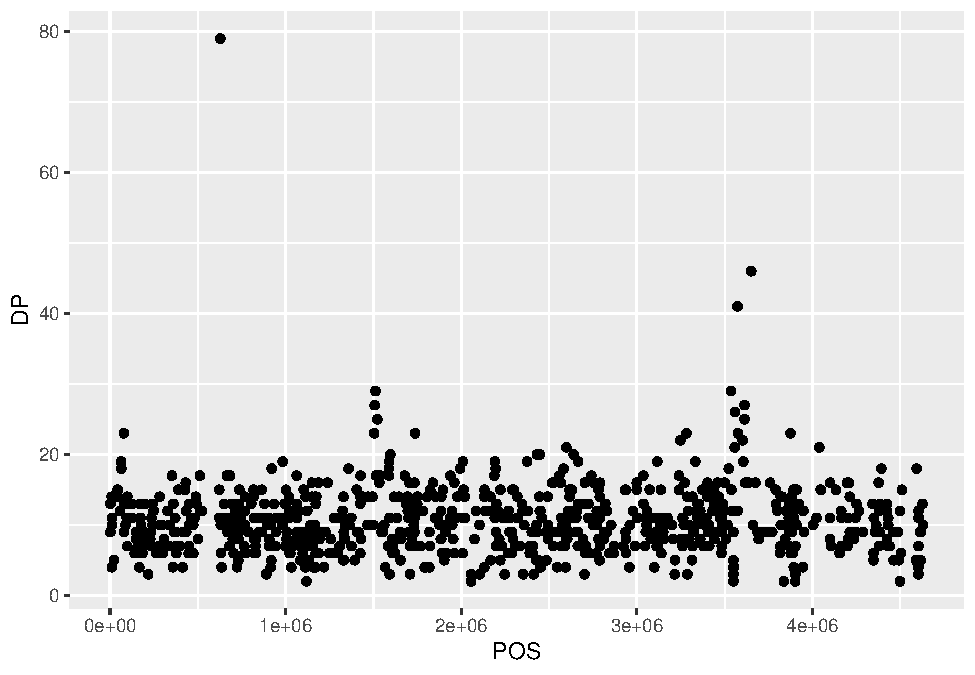
\includegraphics{IntroRWorkshop_files/figure-latex/unnamed-chunk-97-1.pdf}

The \texttt{+} in the \texttt{ggplot2} package is particularly useful because it allows you to modify existing \texttt{ggplot} objects. This means you can easily set up plot templates and conveniently explore different types of plots, so the above plot can also be generated with code like this:

\begin{Shaded}
\begin{Highlighting}[]
\CommentTok{\# Assign plot to a variable}
\NormalTok{coverage\_plot }\OtherTok{\textless{}{-}} \FunctionTok{ggplot}\NormalTok{(}\AttributeTok{data =}\NormalTok{ variants, }\FunctionTok{aes}\NormalTok{(}\AttributeTok{x =}\NormalTok{ POS, }\AttributeTok{y =}\NormalTok{ DP))}

\CommentTok{\# Draw the plot}
\NormalTok{coverage\_plot }\SpecialCharTok{+}
    \FunctionTok{geom\_point}\NormalTok{()}
\end{Highlighting}
\end{Shaded}

Notes:

\begin{itemize}
\tightlist
\item
  Anything you put in the \texttt{ggplot()} function can be seen by any geom layers that you add (i.e., these are universal plot settings). This includes the x- and y-axis mapping you set up in \texttt{aes()}.
\item
  You can also specify mappings for a given geom independently of the mappings defined globally in the \texttt{ggplot()} function.
\item
  The \texttt{+} sign used to add new layers must be placed at the end of the line containing the previous layer. If, instead, the \texttt{+} sign is added at the beginning of the line containing the new layer, \texttt{ggplot2} will not add the new layer and will return an error message.
\end{itemize}

\begin{Shaded}
\begin{Highlighting}[]
\CommentTok{\# This is the correct syntax for adding layers}
\NormalTok{coverage\_plot }\SpecialCharTok{+}
  \FunctionTok{geom\_point}\NormalTok{()}

\CommentTok{\# This will not add the new layer and will return an error message}
\NormalTok{coverage\_plot}
  \SpecialCharTok{+} \FunctionTok{geom\_point}\NormalTok{()}
\end{Highlighting}
\end{Shaded}

\hypertarget{brain-teaser-2}{%
\subsubsection*{Brain Teaser}\label{brain-teaser-2}}
\addcontentsline{toc}{subsubsection}{Brain Teaser}

Can you add multiple geom\_ layers to the same plot?
A Yes
B No

\hypertarget{principles-of-effective-display}{%
\subsection*{Principles of effective display}\label{principles-of-effective-display}}
\addcontentsline{toc}{subsection}{Principles of effective display}

SOURCE: (Whitlock \& Schluter, The Analysis of Biological Data){[}\url{http://whitlockschluter.zoology.ubc.ca/}{]}

We will follow these metrics to create and evaluate figures:
1. Show the data
2. Make patterns in the data easy to see
3. Represent magnitudes honestly
4. Draw graphical elements clearly, minimizing clutter

\hypertarget{exercise-2}{%
\subsubsection*{EXERCISE}\label{exercise-2}}
\addcontentsline{toc}{subsubsection}{EXERCISE}

Create a scatter plot (using the \texttt{geom\_point()} function for quality (\texttt{QUAL}) versus coverage depth (\texttt{DP}).

\hypertarget{building-plots-iteratively}{%
\subsection*{Building plots iteratively}\label{building-plots-iteratively}}
\addcontentsline{toc}{subsection}{Building plots iteratively}

Building plots with \texttt{ggplot2} is typically an iterative process. We start by defining the dataset we'll use, lay out the axes, and choose a geom:

\begin{Shaded}
\begin{Highlighting}[]
\FunctionTok{ggplot}\NormalTok{(}\AttributeTok{data =}\NormalTok{ variants, }\FunctionTok{aes}\NormalTok{(}\AttributeTok{x =}\NormalTok{ POS, }\AttributeTok{y =}\NormalTok{ DP)) }\SpecialCharTok{+}
  \FunctionTok{geom\_point}\NormalTok{()}
\end{Highlighting}
\end{Shaded}

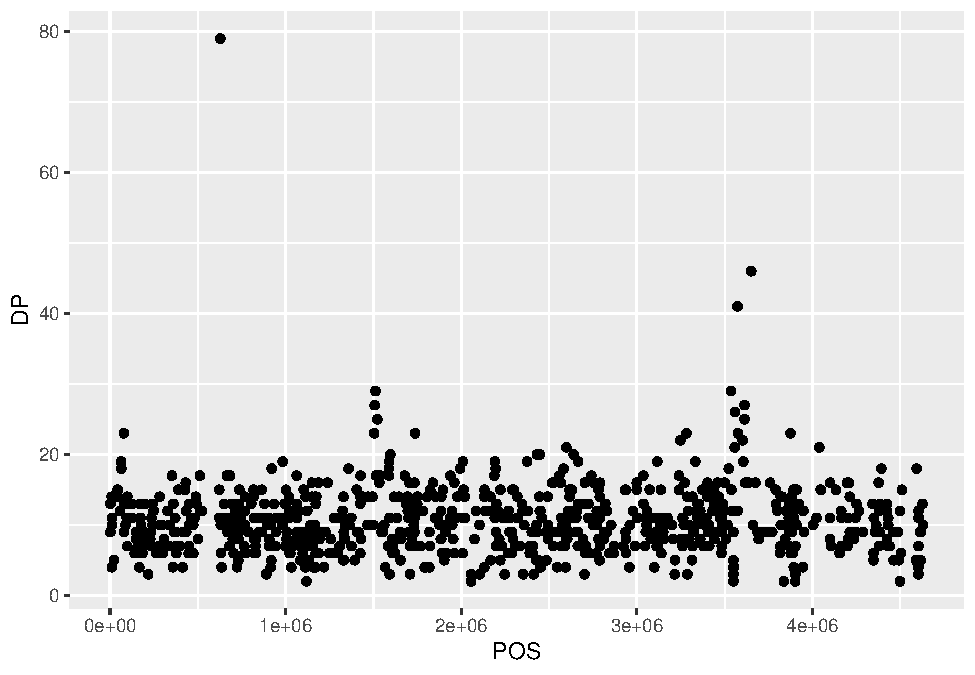
\includegraphics{IntroRWorkshop_files/figure-latex/unnamed-chunk-100-1.pdf}

Then, we start modifying this plot to extract more information from it. For instance, we can add transparency (\texttt{alpha}) to avoid overplotting:

\begin{Shaded}
\begin{Highlighting}[]
\FunctionTok{ggplot}\NormalTok{(}\AttributeTok{data =}\NormalTok{ variants, }\FunctionTok{aes}\NormalTok{(}\AttributeTok{x =}\NormalTok{ POS, }\AttributeTok{y =}\NormalTok{ DP)) }\SpecialCharTok{+}
    \FunctionTok{geom\_point}\NormalTok{(}\AttributeTok{alpha =} \FloatTok{0.5}\NormalTok{)}
\end{Highlighting}
\end{Shaded}

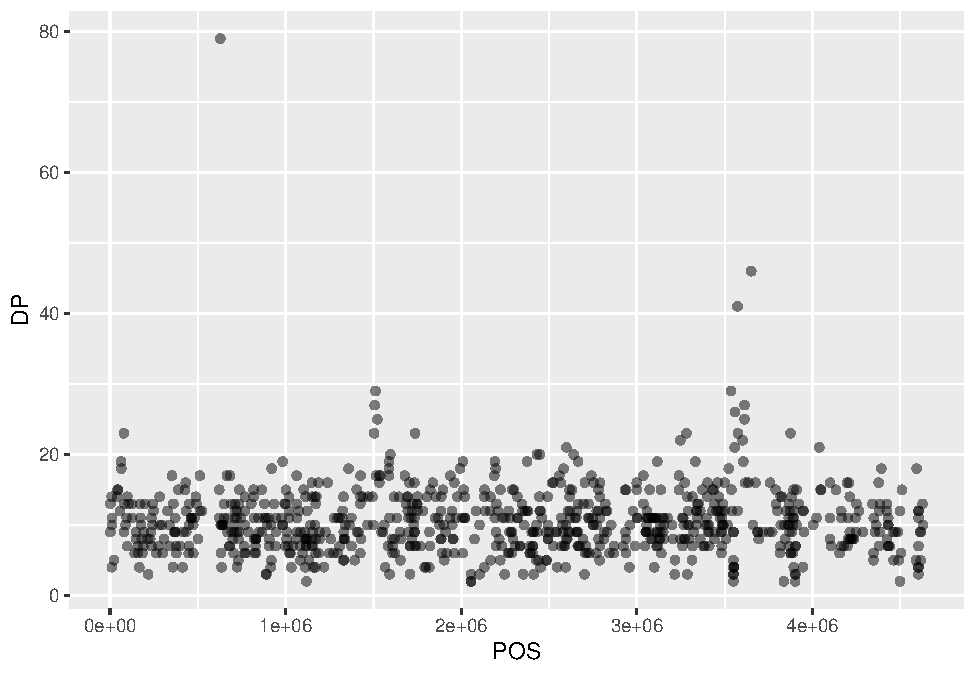
\includegraphics{IntroRWorkshop_files/figure-latex/unnamed-chunk-101-1.pdf}

We can also add colors for all the points:

\begin{Shaded}
\begin{Highlighting}[]
\FunctionTok{ggplot}\NormalTok{(}\AttributeTok{data =}\NormalTok{ variants, }\FunctionTok{aes}\NormalTok{(}\AttributeTok{x =}\NormalTok{ POS, }\AttributeTok{y =}\NormalTok{ DP)) }\SpecialCharTok{+}
  \FunctionTok{geom\_point}\NormalTok{(}\AttributeTok{alpha =} \FloatTok{0.5}\NormalTok{, }\AttributeTok{color =} \StringTok{"blue"}\NormalTok{)}
\end{Highlighting}
\end{Shaded}

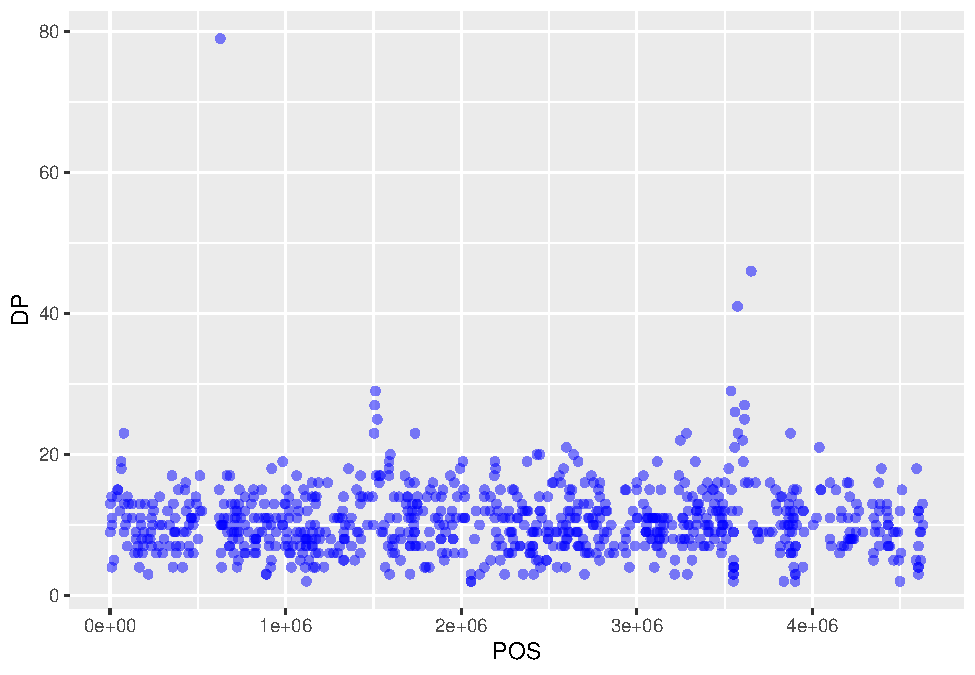
\includegraphics{IntroRWorkshop_files/figure-latex/unnamed-chunk-102-1.pdf}

Or to color each species in the plot differently, you could use a vector as an input to the argument color. \texttt{ggplot2} will provide a different color corresponding to different values in the vector. Here is an example where we color with \texttt{sample\_id}:

\begin{Shaded}
\begin{Highlighting}[]
\FunctionTok{ggplot}\NormalTok{(}\AttributeTok{data =}\NormalTok{ variants, }\FunctionTok{aes}\NormalTok{(}\AttributeTok{x =}\NormalTok{ POS, }\AttributeTok{y =}\NormalTok{ DP, }\AttributeTok{color =}\NormalTok{ sample\_id)) }\SpecialCharTok{+}
  \FunctionTok{geom\_point}\NormalTok{(}\AttributeTok{alpha =} \FloatTok{0.5}\NormalTok{)}
\end{Highlighting}
\end{Shaded}

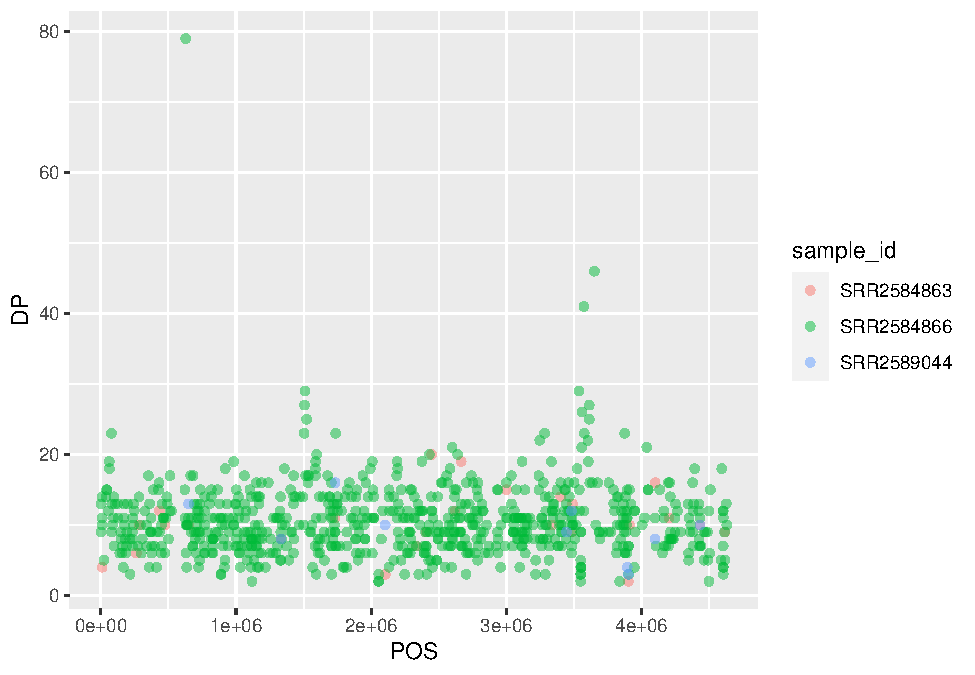
\includegraphics{IntroRWorkshop_files/figure-latex/unnamed-chunk-103-1.pdf}

Notice that we can change the geom layer and colors will be still determined by \texttt{sample\_id}:

\begin{Shaded}
\begin{Highlighting}[]
\FunctionTok{ggplot}\NormalTok{(}\AttributeTok{data =}\NormalTok{ variants, }\FunctionTok{aes}\NormalTok{(}\AttributeTok{x =}\NormalTok{ POS, }\AttributeTok{y =}\NormalTok{ DP, }\AttributeTok{color =}\NormalTok{ sample\_id)) }\SpecialCharTok{+}
  \FunctionTok{geom\_jitter}\NormalTok{(}\AttributeTok{alpha =} \FloatTok{0.5}\NormalTok{)}
\end{Highlighting}
\end{Shaded}

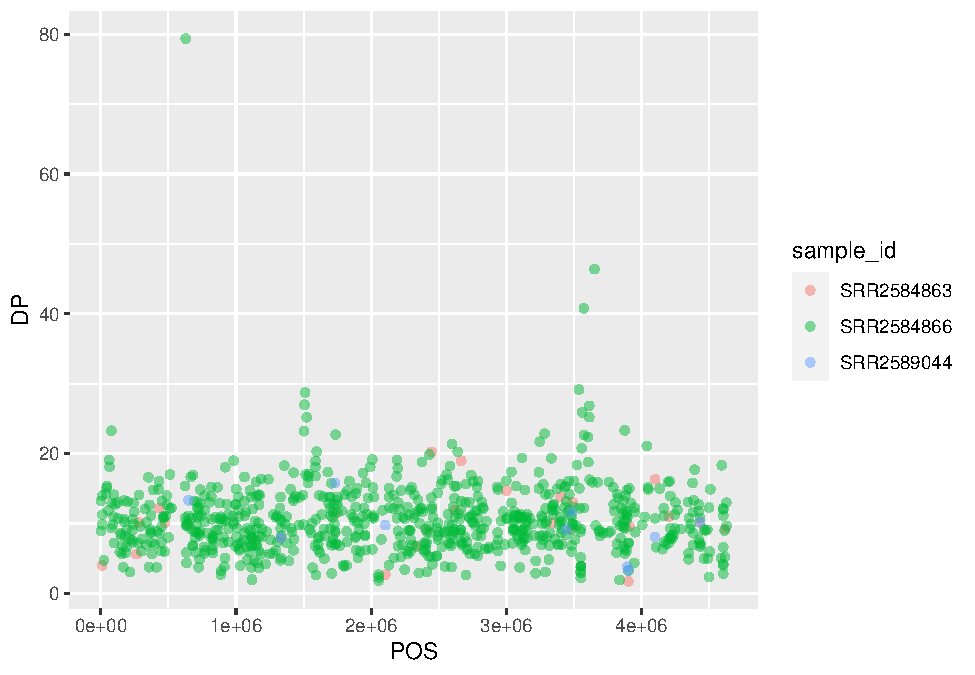
\includegraphics{IntroRWorkshop_files/figure-latex/unnamed-chunk-104-1.pdf}

To make our plot more readable, we can add axis labels:

\begin{Shaded}
\begin{Highlighting}[]
\FunctionTok{ggplot}\NormalTok{(}\AttributeTok{data =}\NormalTok{ variants, }\FunctionTok{aes}\NormalTok{(}\AttributeTok{x =}\NormalTok{ POS, }\AttributeTok{y =}\NormalTok{ DP, }\AttributeTok{color =}\NormalTok{ sample\_id)) }\SpecialCharTok{+}
  \FunctionTok{geom\_jitter}\NormalTok{(}\AttributeTok{alpha =} \FloatTok{0.5}\NormalTok{) }\SpecialCharTok{+}
  \FunctionTok{labs}\NormalTok{(}\AttributeTok{x =} \StringTok{"Base Pair Position"}\NormalTok{,}
       \AttributeTok{y =} \StringTok{"Read Depth (DP)"}\NormalTok{)}
\end{Highlighting}
\end{Shaded}

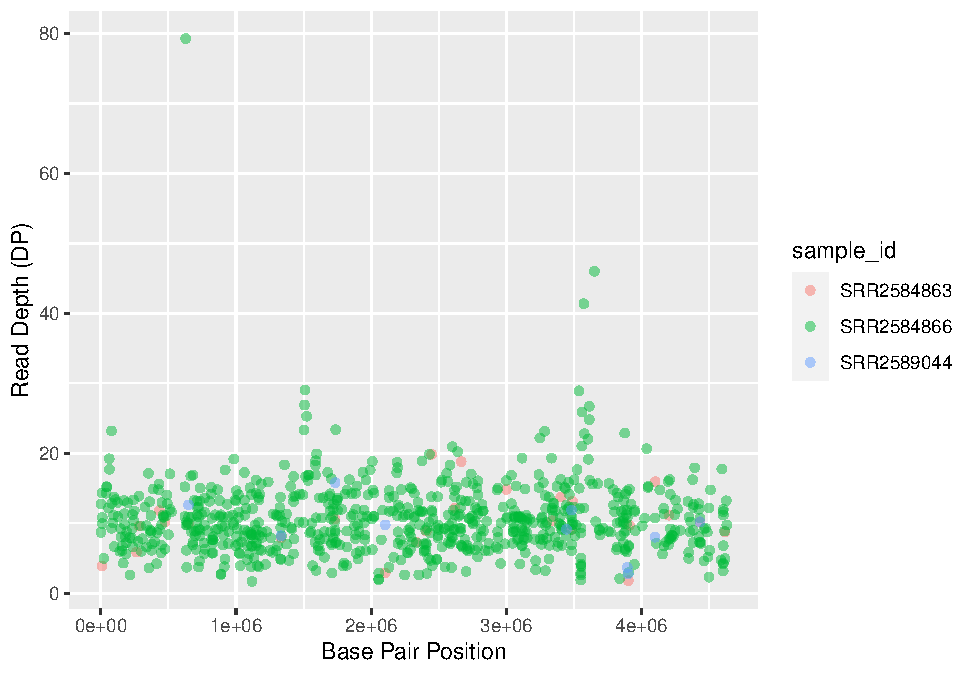
\includegraphics{IntroRWorkshop_files/figure-latex/unnamed-chunk-105-1.pdf}

\hypertarget{exercise-3}{%
\subsubsection*{EXERCISE}\label{exercise-3}}
\addcontentsline{toc}{subsubsection}{EXERCISE}

Create a scatter plot of mapping quality (\texttt{MQ}) over position (\texttt{POS}) with the samples showing in different colors. Make sure to give your plot relevant axis labels.

\hypertarget{faceting}{%
\section{Faceting}\label{faceting}}

\texttt{ggplot2} has a special technique called faceting that allows the user to split one plot into multiple plots based on a factor included in the dataset. We will use it to split our mapping quality plot into three panels, one for each sample.

\begin{Shaded}
\begin{Highlighting}[]
\FunctionTok{ggplot}\NormalTok{(}\AttributeTok{data =}\NormalTok{ variants, }\FunctionTok{aes}\NormalTok{(}\AttributeTok{x =}\NormalTok{ POS, }\AttributeTok{y =}\NormalTok{ MQ, }\AttributeTok{color =}\NormalTok{ sample\_id)) }\SpecialCharTok{+}
 \FunctionTok{geom\_point}\NormalTok{() }\SpecialCharTok{+}
 \FunctionTok{labs}\NormalTok{(}\AttributeTok{x =} \StringTok{"Base Pair Position"}\NormalTok{,}
      \AttributeTok{y =} \StringTok{"Mapping Quality (MQ)"}\NormalTok{) }\SpecialCharTok{+}
 \FunctionTok{facet\_grid}\NormalTok{(. }\SpecialCharTok{\textasciitilde{}}\NormalTok{ sample\_id)}
\end{Highlighting}
\end{Shaded}

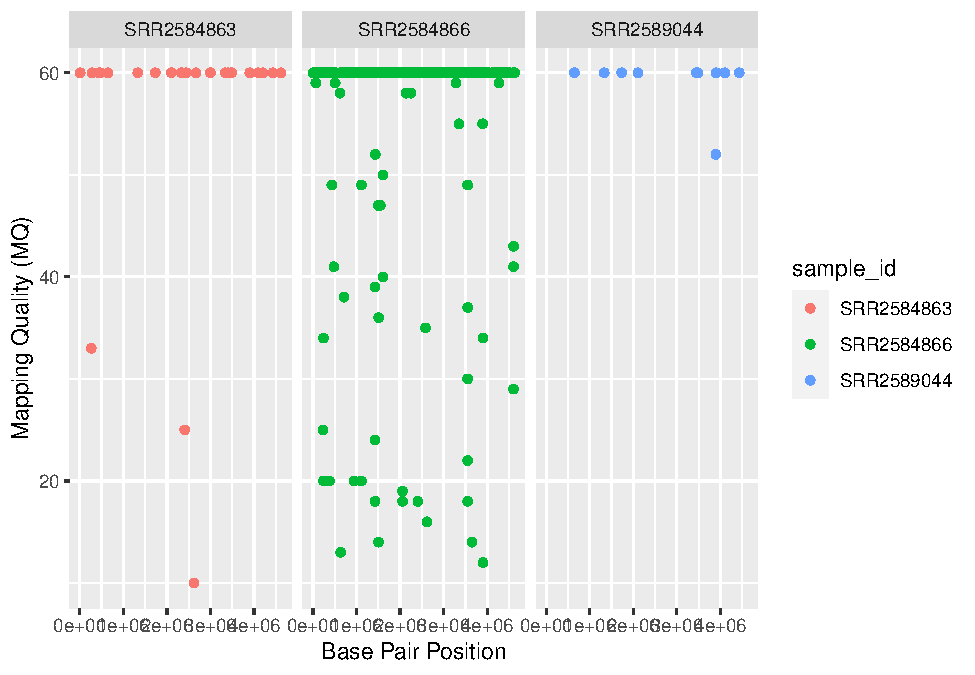
\includegraphics{IntroRWorkshop_files/figure-latex/unnamed-chunk-106-1.pdf}

This looks ok, but it would be easier to read if the plot facets were stacked vertically rather than horizontally. The \texttt{facet\_grid} geometry allows you to explicitly specify how you want your plots to be arranged via formula notation (\texttt{rows\ \textasciitilde{}\ columns}); a \texttt{.} can be used as a placeholder that indicates only one row or column).

\begin{Shaded}
\begin{Highlighting}[]
\FunctionTok{ggplot}\NormalTok{(}\AttributeTok{data =}\NormalTok{ variants, }\FunctionTok{aes}\NormalTok{(}\AttributeTok{x =}\NormalTok{ POS, }\AttributeTok{y =}\NormalTok{ MQ, }\AttributeTok{color =}\NormalTok{ sample\_id)) }\SpecialCharTok{+}
 \FunctionTok{geom\_point}\NormalTok{() }\SpecialCharTok{+}
 \FunctionTok{labs}\NormalTok{(}\AttributeTok{x =} \StringTok{"Base Pair Position"}\NormalTok{,}
      \AttributeTok{y =} \StringTok{"Mapping Quality (MQ)"}\NormalTok{) }\SpecialCharTok{+}
 \FunctionTok{facet\_grid}\NormalTok{(sample\_id }\SpecialCharTok{\textasciitilde{}}\NormalTok{ .)}
\end{Highlighting}
\end{Shaded}

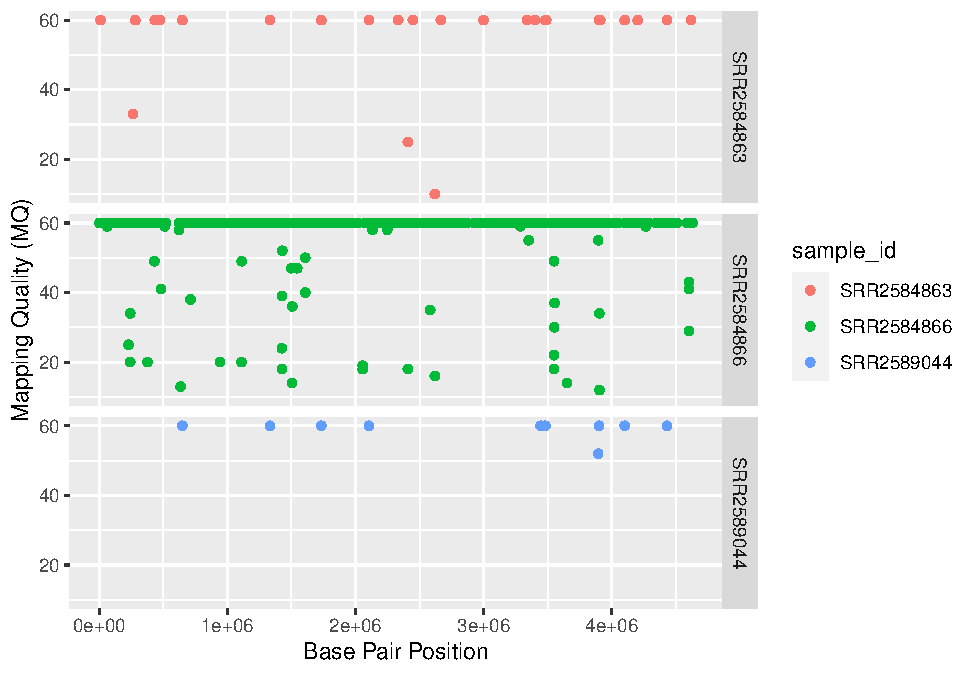
\includegraphics{IntroRWorkshop_files/figure-latex/unnamed-chunk-107-1.pdf}

Usually plots with white background look more readable when printed. We can set the background to white using the function \texttt{theme\_bw()}. Additionally, you can remove the grid:

\begin{Shaded}
\begin{Highlighting}[]
\FunctionTok{ggplot}\NormalTok{(}\AttributeTok{data =}\NormalTok{ variants, }\FunctionTok{aes}\NormalTok{(}\AttributeTok{x =}\NormalTok{ POS, }\AttributeTok{y =}\NormalTok{ MQ, }\AttributeTok{color =}\NormalTok{ sample\_id)) }\SpecialCharTok{+}
  \FunctionTok{geom\_point}\NormalTok{() }\SpecialCharTok{+}
  \FunctionTok{labs}\NormalTok{(}\AttributeTok{x =} \StringTok{"Base Pair Position"}\NormalTok{,}
       \AttributeTok{y =} \StringTok{"Mapping Quality (MQ)"}\NormalTok{) }\SpecialCharTok{+}
  \FunctionTok{facet\_grid}\NormalTok{(sample\_id }\SpecialCharTok{\textasciitilde{}}\NormalTok{ .) }\SpecialCharTok{+}
  \FunctionTok{theme\_bw}\NormalTok{() }\SpecialCharTok{+}
  \FunctionTok{theme}\NormalTok{(}\AttributeTok{panel.grid =} \FunctionTok{element\_blank}\NormalTok{())}
\end{Highlighting}
\end{Shaded}

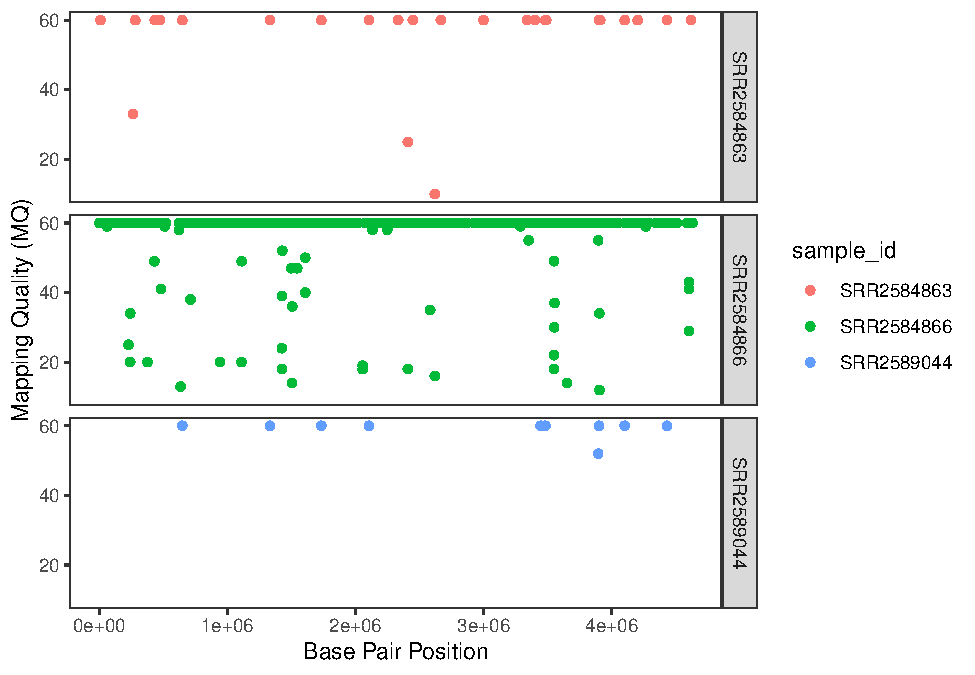
\includegraphics{IntroRWorkshop_files/figure-latex/unnamed-chunk-108-1.pdf}

\hypertarget{exercise-4}{%
\subsubsection*{EXERCISE}\label{exercise-4}}
\addcontentsline{toc}{subsubsection}{EXERCISE}

Use what you just learned to create a scatter plot of PHRED scaled quality (\texttt{QUAL}) over position (\texttt{POS}) with the samples showing in different colors. Make sure to give your plot relevant axis labels.

\hypertarget{barplots}{%
\section{Barplots}\label{barplots}}

We can create barplots using the \texttt{geom\_bar} geom. Let's make a barplot showing the number of variants for each sample that are indels.

\begin{Shaded}
\begin{Highlighting}[]
\FunctionTok{ggplot}\NormalTok{(}\AttributeTok{data =}\NormalTok{ variants, }\FunctionTok{aes}\NormalTok{(}\AttributeTok{x =}\NormalTok{ INDEL, }\AttributeTok{fill =}\NormalTok{ sample\_id)) }\SpecialCharTok{+}
  \FunctionTok{geom\_bar}\NormalTok{() }\SpecialCharTok{+}
  \FunctionTok{facet\_grid}\NormalTok{(sample\_id }\SpecialCharTok{\textasciitilde{}}\NormalTok{ .)}
\end{Highlighting}
\end{Shaded}

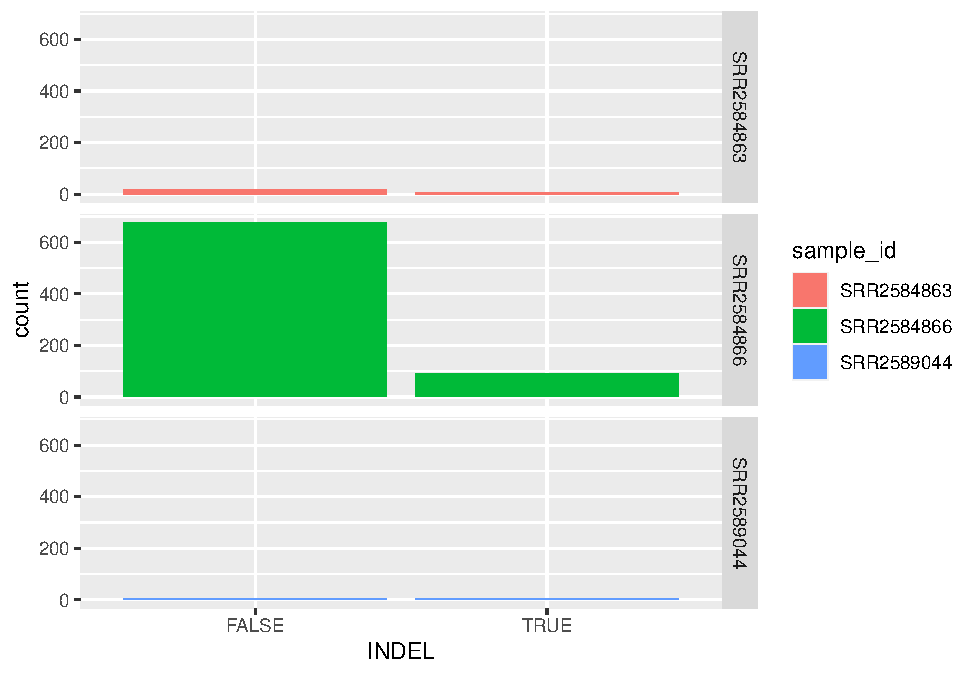
\includegraphics{IntroRWorkshop_files/figure-latex/unnamed-chunk-109-1.pdf}

\hypertarget{exercise-5}{%
\subsubsection*{EXERCISE}\label{exercise-5}}
\addcontentsline{toc}{subsubsection}{EXERCISE}

Since we already have the sample\_id labels on the individual plot facets, we don't need the legend. Use the help file for \texttt{geom\_bar} and any other online resources you want to use to remove the legend from the plot.

\hypertarget{histograms}{%
\section{Histograms}\label{histograms}}

Sometimes it can be useful to plot a single variable at a time. Usually this is for exploratory purposes - to get a feel for a variable. To do this, use the \texttt{geom\_histogram()} function. For example, to look at the distribution of Qualities:

\begin{Shaded}
\begin{Highlighting}[]
\FunctionTok{ggplot}\NormalTok{(}\AttributeTok{data =}\NormalTok{ variants, }\FunctionTok{aes}\NormalTok{(QUAL)) }\SpecialCharTok{+}
  \FunctionTok{geom\_histogram}\NormalTok{()}
\end{Highlighting}
\end{Shaded}

\begin{verbatim}
## `stat_bin()` using `bins = 30`. Pick better value with `binwidth`.
\end{verbatim}

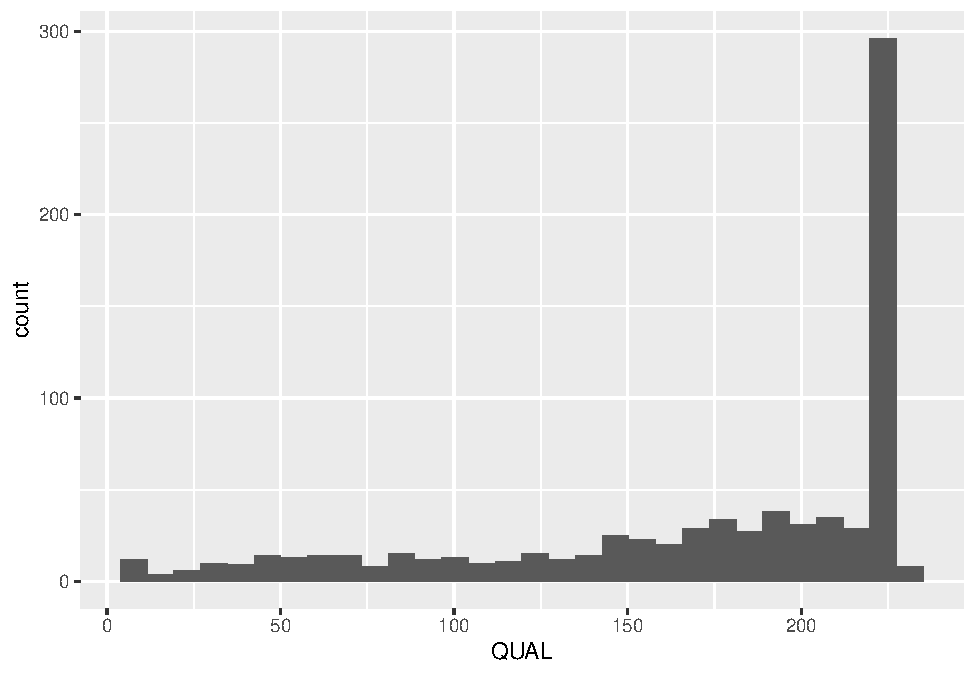
\includegraphics{IntroRWorkshop_files/figure-latex/unnamed-chunk-110-1.pdf}

R is giving us a warning. We can choose to ignore this if we are able to see what we want in the plot. Otherwise, we can change the \texttt{binwidth} by using the binwidth argument:

\begin{Shaded}
\begin{Highlighting}[]
\FunctionTok{ggplot}\NormalTok{(}\AttributeTok{data =}\NormalTok{ variants, }\FunctionTok{aes}\NormalTok{(QUAL)) }\SpecialCharTok{+}
  \FunctionTok{geom\_histogram}\NormalTok{(}\AttributeTok{binwidth =} \DecValTok{5}\NormalTok{)}
\end{Highlighting}
\end{Shaded}

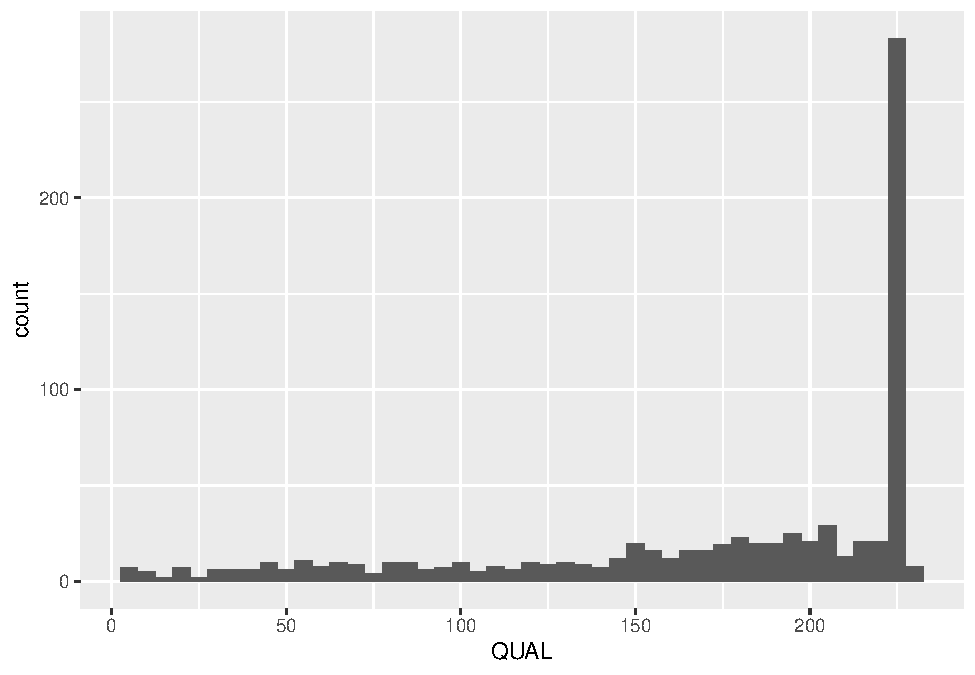
\includegraphics{IntroRWorkshop_files/figure-latex/unnamed-chunk-111-1.pdf}

\hypertarget{exercise-6}{%
\subsubsection*{EXERCISE}\label{exercise-6}}
\addcontentsline{toc}{subsubsection}{EXERCISE}

Create a plot that shows the distribution of Read Depth (DP) for each sample separately.

Bonus challenge. Create this plot for only two of the three samples IDs - the two with many fewer variants.

\hypertarget{boxplots}{%
\section{Boxplots}\label{boxplots}}

When there are a large number of values for a certain variable (like for one of the samples above), boxplots can be a useful way to display summary statistics like the median, and ``spread'' of a variable.

\hypertarget{the-five-number-summary}{%
\subsection*{The Five Number Summary}\label{the-five-number-summary}}
\addcontentsline{toc}{subsection}{The Five Number Summary}

The five number summary gives a quick look at the features of numerical variables. It consists of the variables:

\begin{itemize}
\tightlist
\item
  minimum
\item
  1st quartile
\item
  median
\item
  3rd quartile
\item
  maximum
\end{itemize}

\textbf{QUANTILES:} The \emph{pth} percentile of a data set sorted from smallest to largest is the value such that \emph{p} percent of the data are at or below this value. The quartiles are special percentiles; the 1st quartile is the 25th percentile, and the 3rd quartile is the 75th percentile. The median is also a quartile -- it is the 50th percentile.

Within these five numbers is a lot of useful data!

\begin{itemize}
\tightlist
\item
  the median gives a measure of the center of the data
\item
  the minimum and maximum give the range of the data
\item
  the 1st and 3rd quartiles give a sense of the spread of the data, especially when compared to the minimum, maximum, and median
\end{itemize}

To create a boxplot, use the \texttt{geom\_boxplot()} function:

\begin{Shaded}
\begin{Highlighting}[]
\FunctionTok{ggplot}\NormalTok{(}\AttributeTok{data =}\NormalTok{ variants, }\FunctionTok{aes}\NormalTok{(}\AttributeTok{x =}\NormalTok{ sample\_id, }\AttributeTok{y =}\NormalTok{ DP)) }\SpecialCharTok{+}
  \FunctionTok{geom\_boxplot}\NormalTok{()}
\end{Highlighting}
\end{Shaded}

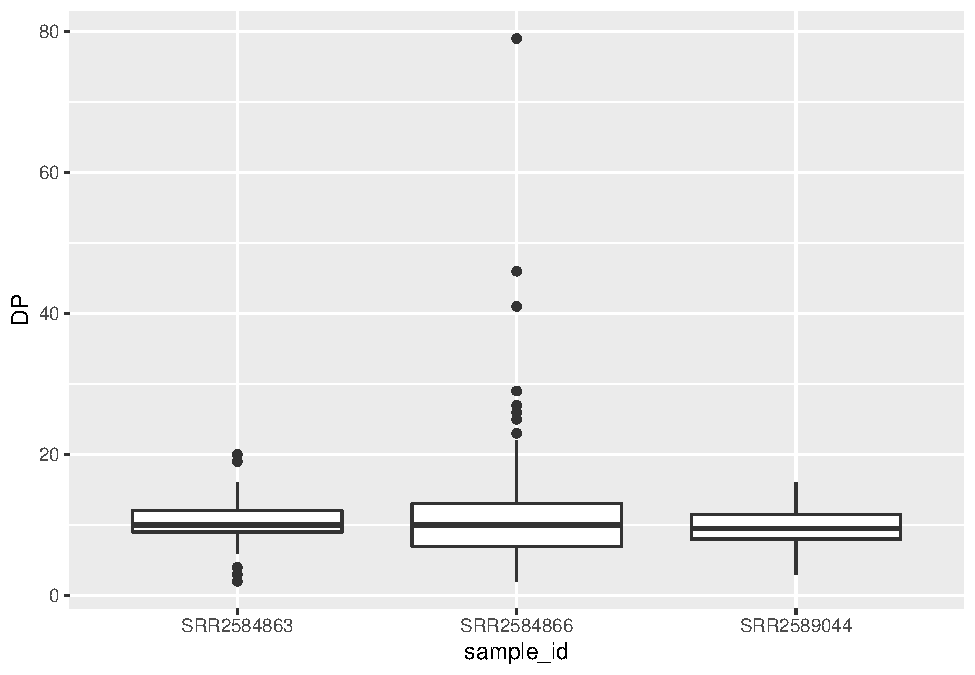
\includegraphics{IntroRWorkshop_files/figure-latex/unnamed-chunk-112-1.pdf}

\hypertarget{exercise-7}{%
\subsubsection*{EXERCISE}\label{exercise-7}}
\addcontentsline{toc}{subsubsection}{EXERCISE}

\begin{enumerate}
\def\labelenumi{\arabic{enumi}.}
\tightlist
\item
  Change the colour of each box in the above plot to match the sample\_id colours in the plots above.
\item
  Log transform the y-axis.
\end{enumerate}

Bonus challenge: Change the name of the legend to ``Sample ID''.

\hypertarget{themes}{%
\section{Themes}\label{themes}}

In addition to \texttt{theme\_bw()}, which changes the plot background to white, \texttt{ggplot2} comes with several other themes which can be useful to quickly change the look of your visualization. The complete list of themes is available at \url{https://ggplot2.tidyverse.org/reference/ggtheme.html}. \texttt{theme\_minimal()} and \texttt{theme\_light()} are popular, and \texttt{theme\_void()} can be useful as a starting point to create a new hand-crafted theme.

The \texttt{ggthemes} package provides a wide variety of options (including an Excel 2003 theme). The \texttt{ggplot2} \href{https://www.ggplot2-exts.org}{extensions website} provides a list of packages that extend the capabilities of \texttt{ggplot2}, including additional themes.

\hypertarget{project}{%
\chapter{Project}\label{project}}

\hypertarget{introduction-1}{%
\section*{Introduction}\label{introduction-1}}
\addcontentsline{toc}{section}{Introduction}

The data we're going to work with comes from a yeast microarray experiment \href{http://www.molbiolcell.org/content/19/1/352.abstract}{(Brauer, 2008)} where the authors measured gene expression in 36 chemostat cultures where growth was limited by one of six nutrients (glucose, ammonium, sulfate, phosphate, uracil, or leucine) at 6 different growth rates.

The R world is full of niche tools designed for a specific problem or data type. This is particularly true for Bioconductor and genomics analysis. RNA-seq is a good example where all data import, analysis, and even plotting is done with custom packages and functions designed for gene expression data. Analysis of microbiome data with phyloseq is another example. Now this is not a bad thing and can enable simple, rapid analysis. Yet the point of learning a programming language like R is so you can take back control of your analysis and put the tools to work for your specific problem.

For this project we're going to take some genomic data and analyze it with the tools that we've been learning. The take-away from this project to make the tools work for you instead of you working for them. Data, genomic or not, is still data and we can use the tools available to us in R to gain valuable insights.

\hypertarget{task-0-download-the-data}{%
\section*{Task 0: Download the data}\label{task-0-download-the-data}}
\addcontentsline{toc}{section}{Task 0: Download the data}

You can find the data for download from dropbox \href{https://www.dropbox.com/sh/jqu2ixdug5el66f/AAB86klTjyR-JgW502KXwbj1a?dl=0}{here}.

\hypertarget{task-1-data-import-and-examination}{%
\section*{Task 1: Data import and examination}\label{task-1-data-import-and-examination}}
\addcontentsline{toc}{section}{Task 1: Data import and examination}

The first task of almost all analysis is to get the data into R and spend a little time understanding it's structure. Although you may be tempted to rush into an analysis it pays to take a bit of time to understand what you are working with and do some cleaning before you dive in too deep. This is important help you avoid costly mistakes and wasted time downstream.

The data file you'll be using is \texttt{Brauer2008\_DataSet1.csv} and although it is pre-processed it will still need some work to get it ready to use.

Your goal is get the data loaded into R and answer the following questions:

\begin{enumerate}
\def\labelenumi{\arabic{enumi}.}
\tightlist
\item
  How many rows and columns are there?
\item
  What do the rows and columns represent?
\item
  On first glimpse do the column \textbf{datatypes} look correct?
\item
  What about column names?
\item
  Is this data tidy? Why or why not?
\end{enumerate}

As you look through the data start thinking about what steps you'll need to get it into a workable state.

\hypertarget{task-2-data-tidying}{%
\section*{Task 2: Data Tidying}\label{task-2-data-tidying}}
\addcontentsline{toc}{section}{Task 2: Data Tidying}

Never underestimate the amount of time and effort it will take to tame a wild dataset into something usable. Even if someone has already processed and ``cleaned'' the data before you (such as our current dataset) it is likely that you will need to spend some time fiddling with it for your particular needs (or for a particular function you want to use).

You've learned about the tidy data concepts, now it's time to put them into practice. The first and most important step is decide what, if any tidying needs to be done. Recall that:

\begin{itemize}
\tightlist
\item
  Each variable forms a column.
\item
  Each observation forms a row.
\item
  Each type of observational unit forms a table.
\end{itemize}

Questions to answer:

\begin{enumerate}
\def\labelenumi{\arabic{enumi}.}
\tightlist
\item
  Which \textbf{column} contains multiple variables? Split it up so each column represents a single variable. (Hint: for the \texttt{sep} argument, use \texttt{sep\ =\ "\textbackslash{}\textbackslash{}\textbar{}\textbackslash{}\textbackslash{}\textbar{}"}. But think about why!)
\item
  The \texttt{GWEIGHT}, \texttt{GID}, and \texttt{YORF} columns we also won't need so you can get rid of those.
\item
  Is this data in \textbf{long} format? How can you fix that?
\item
  Do you have any columns that have multiple variables? Be sure to fix any before you move on.
\end{enumerate}

Try to code all the cleaning steps as a single pipeline. Remember the \texttt{separate()} and \texttt{gather()} functions from the tidyr package.

\textbf{Bonus:} Your cleaning steps may have left some variables with extra white space at the end. Hint: Using \texttt{mutate\_at()} with the \texttt{str\_trim} option, see if you can clean these up.

\hypertarget{task-3-plots}{%
\section*{Task 3: Plots}\label{task-3-plots}}
\addcontentsline{toc}{section}{Task 3: Plots}

Whew! Alright, that's done, but now you might asking why spend all that time cleaning up the data. Hopefully you should be able to answer that question by now but moving on to making some plots will help make it even more clear.

In a typical analysis you wouldn't necessarily know which gene(s) to start looking at and would want to start with some more exploratory analysis. However, to practice our plotting and analysis let's focus on a few pre-picked genes and pathways.

\begin{enumerate}
\def\labelenumi{\arabic{enumi}.}
\tightlist
\item
  Filter your now cleaned data to contain only the gene LEU1.
\item
  Make a plot of the expression of this gene at various growth rates. Use colour to distinguish the different nutrients.
\item
  What are some conclusions you can make from this data?
\item
  What biological process is LEU1 classified as?
\item
  Filter your cleaned data for all genes that are in the same biological process as LEU!.
\item
  Make a plot of these genes, the same as you had for LEU1 but faceted by gene.
\item
  Do any of the other genes follow the same pattern as LEU1?\\
\item
  Customize your plot a bit by changing the colour palette to one of the RColorBrewer palettes. Explore some of the other themes available (\texttt{theme\_bw()} is particularly nice). Fix the x-axis and y-axis labels so they look nicer.
\end{enumerate}

\textbf{Bonus:} To increase readability of the plot it can helpful to change those nutrients from letters to full words. Although there are ways to do this directly in ggplot the easiest is to change it in the original data.

\hypertarget{task-4-heatmap}{%
\section*{Task 4: Heatmap}\label{task-4-heatmap}}
\addcontentsline{toc}{section}{Task 4: Heatmap}

Heatmaps are quite popular but generally useless visualisations used frequently in the genomic sciences. They can show a large amount of information in a small space, however, this very feature often renders them useless in terms of interpretability. Yet, for some applications they can be useful and let's face it, your supervisor propbably wants one so it's a good skill to have.

Heatmaps are very straight forward to make with ggplot using \texttt{geom\_tile()} however, one of the more useful features of heatmap is the row and column ordering usually done with hierarchical clustering. This is non-trivial (but not impossible) to implement with ggplot so instead we're going to look at a package specifically designed for these types of heatmaps. There are as many heatmap packages for R as there are heatmaps and you may end up using different packages for different purposes. However, the \texttt{pheatmap} package has a nice balance of features, speed, and ease of use and is the one we'll work with today, although you are free to look at others for your own needs.

To this point much of your training has focused on the concepts of tidy data analysis, which are very powerful and you will come to rely on for much of your work. However, for genomics and other bioinformatics analysis you will often find yourself having to go between the \emph{tidyverse} and other custom formats and datatypes specific to another package or the more traditional R datatypes, particularly the matrix format. In addition to learning how to make a nice heatmap the other main goal of this task is to help you become familar with moving back and forth between different data structures.

Questions to answer:

\begin{enumerate}
\def\labelenumi{\arabic{enumi}.}
\tightlist
\item
  Start by installing the \texttt{pheatmap} package from CRAN. Have a look at the help page for the \texttt{pheatmap()} function. Which argument specifies the data? What format does it need?
\item
  Using what you learned from the help function get the gene expression data into a format that \texttt{pheatmap()} can use. Think about what you want your heatmap to look like - what are the columns and rows?
\item
  Once you've got data in the correct format start by making a simple heatmap with default parameters. Do you like it? Is there anything wrong with it? What would change from a data interpretation perspective? What about from aethetics perspective?
\end{enumerate}

  \bibliography{book.bib,packages.bib}

\end{document}
